\chapter{基于梯度子模型抽取的联邦学习方法} 
\section{引言}
在上一章节中我们基于深度学习中神经元最基础的生物学意义,
就是在生物中神经元的活跃程度代表着其在当前状态下的重要性。
在深度学习的模型中,
将模型在推理过程中前向传播的输出值作为其活跃程度的依据,
这也是上一章节中给不同边缘设备抽取子模型的重要依据。
尽管上一章节中叙述的方法已经取得了很好的成绩,
但确实是仅仅从启发性从整个模型训练过程中的前向传播过程考虑,
没有考虑在整个训练过程中极为重要的反向传播过程的重要性。
在反向传播过程中产生的各个神经元的梯度,
这些梯度信息决定了模型的优化方向。

毫无疑问,
在联邦学习中边缘设备与中心服务器端均是同构模型的话,
模型最终取得效果是好于在资源受限情况下边缘设备训练与
中心服务器侧不同的异构模型,也就是抽取的子模型。
在这个基础之上,
我们可以得到上一章节中的自适应算法并未考虑联邦学习整体的优化方向,
也就是考虑在资源受限的情况下,
自适应抽取子模型算法要做到与边缘设备资源充足情况下,
模型的优化方向也就是梯度更新最为接近,
这样我们就能得到与充足资源情况下相差最少的模型。
反观论文中描述的以前的方法中,
从预先制定规则出发考虑解决问题的策略,
HeteroFL设计了一个可以在资源受限情况下可以运行的系统,
通过按层抽取神经元的可靠稳定的设计;
FedRolex仅仅考虑了在自己抽取规则之下,
保证每个神经元受到的训练次数是一样的,
从而保证模型最终的效果不至于出现很大的波动与偏差。
在上一章节的方法中虽然采用了自适应的方法,
但是仅仅是从前向传播也就是激活值的角度去考虑,
而没有考虑到梯度更新的优化约束。
综上这些方法都从来没有考虑到优化约束的问题。

站在局部与总体优化的角度来看,
本章节提出了一个基于梯度的逼近子模型模型与
服务器侧中心模型优化方向的方法FedGSE。
其核心点在于根据反向传播过程中计算的每层中神经元
梯度,
根据边缘设备的计算能力选择其中梯度绝对值大的组成边缘设备的
子模型,
从而使得子模型与中心侧全局模型更新最为接近。
因为需要在中心侧模型上进行反向传播计算梯度,
边缘设备的计算资源不足以支撑此等规模的运算,
因此创建一个样本量不大的公共数据集,
也就是中心侧数据集使得反向传播的执行过程可以在中心侧运行,
并且仅广播给边缘设备子模型参数即可完成,
降低了中心侧与边缘设备之间的传输通讯量。
总体来说本章节的贡献可以总结如下:
\begin{itemize}
    % yabo 新增
    \item 本文从优化的角度出发,
    指出了子模型本地更新与全局模型之间的差异是导致全局模型收敛效率降低的原因。
    为了缩小这一差距,我们提出了一种新方法FedGSE,该方法选择梯度值较大的神经元,
    以确保全局模型和子模型的最小本地更新差异。    

    \item 我们提供了数学证明,表明在相同训练情境下,
    FedGSE算法能够实现全局模型和子模型之间最小的更新梯度差异。
    这证明了经过训练的子模型参数与全局模型参数最为接近。
    
    \item 为了评估我们提出的方法的有效性,
    我们将其与各种数据集和设置下的最近方法对比。
    大量实验结果表明,FedGSE显著优于其他方法。
    
\end{itemize}



\section{FedGSE算法}
本小节将详细介绍FedGSE方法中的各种细节。
FedGSE采用梯度作为抽取子模型的标准来解决联邦学习资源受限的场景,
首先,
我们需要在中心侧建立一个跟边缘设备数据集相似且包含大部分或者
所有边缘设备需要用到的公共数据集,
这个数据集用来在中心侧执行反向传播来获取各个神经元梯度。
在获得公共数据集前提下,
我们采用SPL或者CSL方法来根据边缘设备的历史模型来预测
与边缘设备数据分布相似的公共子数据集,
具体的SPL和CSL算法可见图\ref{fig:4-2spl_csl},
伪代码见算法\ref{alg:getbackData}与算法\ref{alg:getbackwardData1},
然后使用公共子数据集在中心侧模型上执行反向传播产生梯度来抽取子模型,
可见图\ref{fig:4-2overview}与算法\ref{alg:GetMaskFedDSE}。
之后,
中心侧服务器将模型发送给客户端,
在客户端侧使用边缘设备本身的数据集训练,
从而完成整个模型的训练,
整个FedGSE的整体代码见算法\ref{alg:feddse}。
本小章节从公共数据集构建、相似公共子数据集产生、子模型抽取、
端侧训练以及模型聚合来详细介绍FedGSE算法流程。
本章节所有资源受限情况下联邦学习优化的目标相同,
也就是优化公式\ref{equ:total_fl}与公式\ref{equ:total_fl_ap}。

%ccccccccccccccccccccccccccccccccccccccccccccccccccccccccccccccc
\begin{algorithm}[thbp]
    \caption{FedGSE算法}
    \label{alg:fedgse}
    \begin{algorithmic}[1]
    \Require 全局模型参数 $\mathbf{w}$,
            学习率 $\eta$, 总通讯次数 $T$, 
            所有边缘设备计算能力 $\{r_0, \cdots,r_{N-1}\}$, 
            公共数据集 $\mathbb{D}^P$,
            本地客户端训练次数$E$
    \Ensure $T$轮的全局模型参数$\mathbf{w}_{T+1}$
    \State 初始化全局模型参数$\mathbf{w}_1$
    \Procedure{Server-side Optimization}  {}
        \For {对每个轮次 $t \in \{1, \cdots, T \}$}
            \State 随机挑选所有客户端的子集 $\mathcal{N}_t$
            \For {对于每个挑选到的客户端 $n$ \textbf{并行执行}}
                \State 生成相似数据集 $\mathbb{D}^P_n \leftarrow$ \textbf{GetSimilarDataCSL} $(\mathbb{D}^P,\mathbf{w^n})$  or  $\mathbb{D}^P_n \leftarrow$ \textbf{GetSimilarDataSPL} $(\mathbb{D}^P)$  
                \State $\mathbf{M^{n,t}} \leftarrow$ \textbf{GetMask}($r_n$, $\mathbb{D}^P_n$, $\mathbf{w_{t}}$)
                \State 抽取子模型 $\mathbf{w^n_t} \leftarrow \mathbf{w_t} \odot \mathbf{M^{n,t}}$
                \State $\mathbf{w^n_{t+1}} \leftarrow$ \textbf{ClientLocalUpdata}($n$, $\mathbf{w^n_t}$)
            \EndFor
            \State 更新全局模型参数 $\mathbf{w_{t+1}} = \sum_{n \in \mathcal{N}_t} \mathbf{P}^n_t \odot \mathbf{w^n_{t+1}} $
        \EndFor
    \EndProcedure
    
    \Procedure{ClientLocalUpdate}{$n$, $\mathbf{w_t^n}$}
        \State 从服务器接受 $\mathbf{w_t^n}$
        \For{从$1$到$E$迭代轮次$e$}
            \State 在本地数据集上更新本地模型 $\mathbf{w^n_{t,e+1}} = \mathbf{w^n_{t,e}} - \eta \nabla_{\mathbf{w^n_{t,e}}} f_n(\mathbf{w^n_{t,e}})$
        \EndFor
        \State \Return $\mathbf{w^n_{t,E+1}}$
    \EndProcedure
    \end{algorithmic}
\end{algorithm}
%ccccccccccccccccccccccccccccccccccccccccccccccccccccccccccccccc

\subsection{公共数据集构建}
在联邦学习中,
每个客户端的数据都是独特的,
因此只有公共数据集中的数据与大部分客户端中的数据拥有相似的分布,
或者所有客户端的数据分布是公共数据集的一个子集,
才能保证我们在后续在中心侧得到的神经元梯度与
使用客户端数据得到是相近的。
基于这样的前提,我们可以使用三种方法来构建我们的公共数据集:

(1) 鼓励客户上传小部分自己产生的数据集。
边缘侧用户会产生大量的数据,
并不是所有的数据都包含大量的隐私信息,
用户可以自行选择小部分可以被用来处理的信息上传到中心服务器侧
以便提供更好的服务,
这些小部分信息可能占用户本身数据集的百分之一不到。

(2)使用覆盖面积更广的数据集。
因为后面我们使用的方法可以筛选出相似数据集,
因此我们可以收集覆盖范围更广更多的数据来组成更大的数据集,
也就是让客户端中的数据集成为我们收集公共数据集的子集,
这样也能保证我们需要公共数据集的作用。

(3)使用生成式模型生成伪数据。
在边缘设备可以训练生成式模型的前提下,
可以使边缘设备根据自己的数据使得生成式模型生成数据,
然后将这些伪数据上传到中心侧作为公共数据集。


\subsection{边缘侧相似数据集产生策略}
在构建完公共数据集之后,
我们不是使用全部的公共数据集输入全局模型中去产生抽取子模型所需要的梯度。
使用全部的公共数据集首先是效率比较低下,
占用计算资源与时间较多。
其次,
筛选出与客户端数据集分布相似的公共子数据输入全局模型产生的梯度更加
接近在客户端上执行的效果。
因此,
我们需要设定产生分布相似公共子数据集的策略,
保证
\begin{equation}
    \label{eq:sameDataDis}
    P_{\mathbb{D}^P_n} \approx P_{\mathbb{D}_n}
\end{equation}
其中,
$\mathbb{D}_n$ 表示客户端$n$的数据集,
$\mathbb{D}^P_n$ 表示与客户端$n$分布相似的公共子数据集,
$P_{(\cdot)}$ 表是数据分布。
我们使用两种策略来实现从公共数据集中筛选出与客户端分布相似的公共子数据集:
%ppppppppppppppppppppppppppppppppppppppp
\begin{figure}[thbp]
    \centering
    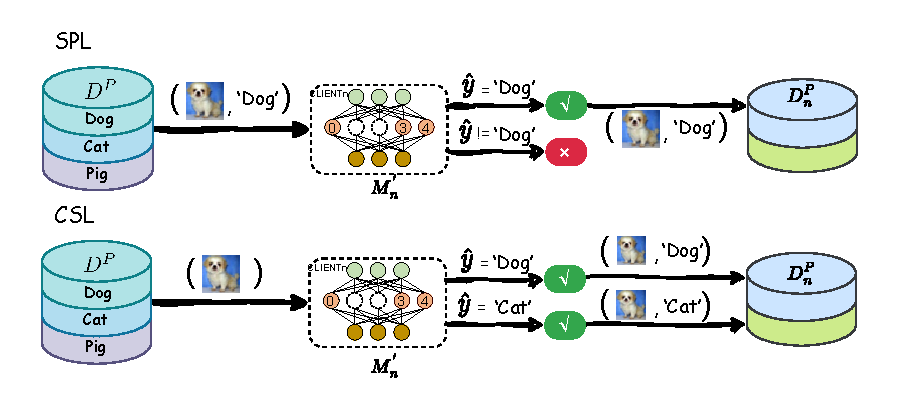
\includegraphics[width=0.9\linewidth]{chapter4/SPL_CSL.pdf}
    \caption{\label{fig:4-2spl_csl}两种产生相似分布数据集的方法}
\end{figure}
%ppppppppppppppppppppppppppppppppppppppp

\textbf{服务器侧挑选有标签数据集}
\text{(\underline{S}erver \underline{P}icks samples through 
\underline{L}abeled dataset SPL) }
在服务器侧我们使用SPL去筛选公共数据集具有真是标签的数据,
具体算法如图\ref{fig:4-2spl_csl}与算法\ref{alg:getbackData}所示。
首先,公共数据集$\mathbb{D}^P$中包含所有客户端所有类别的数据,
将公共数据集中的所有数据都输入到客户端$i$的上次保存在服务器上的模型$M_i^{'}$中,
并预测每条数据在模型$M_i^{'}$中的标签
\begin{equation}
    \label{equ:prelabel}
    \hat{y}_i=f(\mathbf{w}^n; x_i)
\end{equation}
如果客户端历史模型预测正确,
也就是$\hat{y}_i$等于其真实标签$y_i$,
那么将该样本加入到$\mathbb{D}^P_n$中;
相反,
如果预测结果不正确,
那么就将这一条数据抛弃。
客户端历史模型能预测正确说明模型大概率见过这些数据,
也就是说当前数据大概率在客户端数据集的分布之中,
符合我们的挑选的原则,
具体代码如算法\ref{alg:getbackData}所示。
我们使用图\ref{fig:4-2spl_csl}进行详细的讲解,
图中公共数据集包含狗、猫以及猪三类数据,
在SPL方法中,
我们给模型输入了狗的照片以及真是标签“dog”,
这个模型是客户端n在上个轮次中上传到中心侧的最新的模型,
然后模型执行推理过程,
预测输入狗的图片是什么,
如果预测为“dog”就加入到与客户端模型相似分布的公共子数据集中,
否则就直接抛弃。
\begin{algorithm}[thbp]
    \caption{GetSimilarDataSPL}\label{alg:getbackData}
    \begin{algorithmic}[1]
    \Require 公共数据集 $\mathbb{D}^P$, 客户端模型 $\mathbf{w^n}$
    \Ensure 与客户端$n$相似分布的数据集 $\mathbb{D}^P_n$ 
    \Procedure{GetSimilarDataSPL}{$\mathbb{D}^P,\mathbf{w^n}$}
        % \If {$\mathbf{w^n}$ not Initialization}
        %     \State Randomly select $s$ classes to compose subset $\mathcal{L}$ from $\mathcal{C}$ 
        % \Else
        \State 初始化 $\mathbb{D}^P_n=\emptyset$
        \For{对于数据样例 $(x_i,y_i) \in \mathbb{D}^P$}
            \State 预测标签 $\hat{y}_i=f(\mathbf{w}^n; x_i)$
            \If {$\hat{y}_i == y_i$}
               \State 将样例加入 $\mathbb{D}^P_n \gets \mathbb{D}^P_n \cup \{(x_i,y_i)\}$
            \EndIf
        \EndFor
        \State \Return $\mathbb{D}^P_n$
    \EndProcedure
    \end{algorithmic}
\end{algorithm}
%ccccccccccccccccccccccccccccccccccccccccccccccccccccccccccccccc

%ccccccccccccccccccccccccccccccccccccccccccccccccccccccccccccccc
\begin{algorithm}[thbp]
    \caption{GetSimilarDataCSL}\label{alg:getbackwardData1}
    \begin{algorithmic}[1]
    \Require 公共数据集 $\mathbb{D}^P$
    \Ensure 与客户端$n$相似分布的数据集 $\mathbb{D}^P_n$ 
    
    \Procedure{GetSimilarDataCSL}{$\mathbb{D}^P$}
        \State 初始化 $\mathbb{D}^P_n=\emptyset$
        \For{对于每个样例 $x_i \in \mathbb{D}^P$}
            \State 预测标签 $\hat{y}_i=f(\mathbf{w}^n; x_i)$
            \State 将样例加入 $\mathbb{D}^P_n \gets \mathbb{D}^P_n \cup \{(x_i,\hat{y}_i)\}$
        \EndFor
    \EndProcedure
    \end{algorithmic}
\end{algorithm}
%ccccccccccccccccccccccccccccccccccccccccccccccccccccccccccccccc

\textbf{客户模型设定无标签数据集}
(\underline{C}lient sub-model to \underline{S}et 
\underline{L}abels of unlabeled public dataset CSL) 
当在服务器侧使用CSL生成分布相似的公共子模型,
具体介绍如图\ref{fig:4-2spl_csl}和算法\ref{alg:getbackwardData1}所示,
首先,
公共数据集$\mathbb{D}^P$中包含所有类别的数据,
在CSL的算法之下,
这些数据只需要保证存在即可,
而不需要对应的真实标签。
然后将公共数据集中的所有数据输入到模型$M_i^{'}$之中,
跟SPL一样,
这个模型是客户端n最近一次上传给中心侧的模型,
然后使用公式\ref{equ:prelabel}在模型预测输入的数据的标签,
与SPL不同的是,
因为没有真实标签,
我们直接将$\hat{y}_i$作为输入数据的标签,
用来使数据拟合模型分布,
最后将输入数据跟预测标签加入到公共相似分布子数据集中。
我们使用图\ref{fig:4-2spl_csl}下班部分详细介绍,
在图中,
输入的数据是一个狗的照片并且没有给出真实标签,
模型跟在SPL中的一致的,
都是上次客户端n最近上传的,
接着就是给模型去预测这张照片的类别。
在上面的路径中预测这张照片是“dog”,
与我们认知是相同的,
这个时候我们将狗的照片加预测标签“dog”添加到要返回的数据集中。
在第二条路径中,
模型预测出照片的标签是“cat”,
与SPL方法不同的是,
我们不抛弃这种情况下的数据,
因为我们没有真实标签去做对比,
也要讲这条数据也就是狗的照片加预测标签“cat”添加到要返回的数据集中。
其实我们在这一过程要学习的是最近客户端上传模型在本地数据集上学习到的
知识,
我们通过预测过程将知识转移到公共数据集中,
以方便我们得到数据分布相关的梯度。

\subsection{子模型抽取}
%ppppppppppppppppppppppppppppppppppppppp
\begin{figure}[thbp]
    \centering
    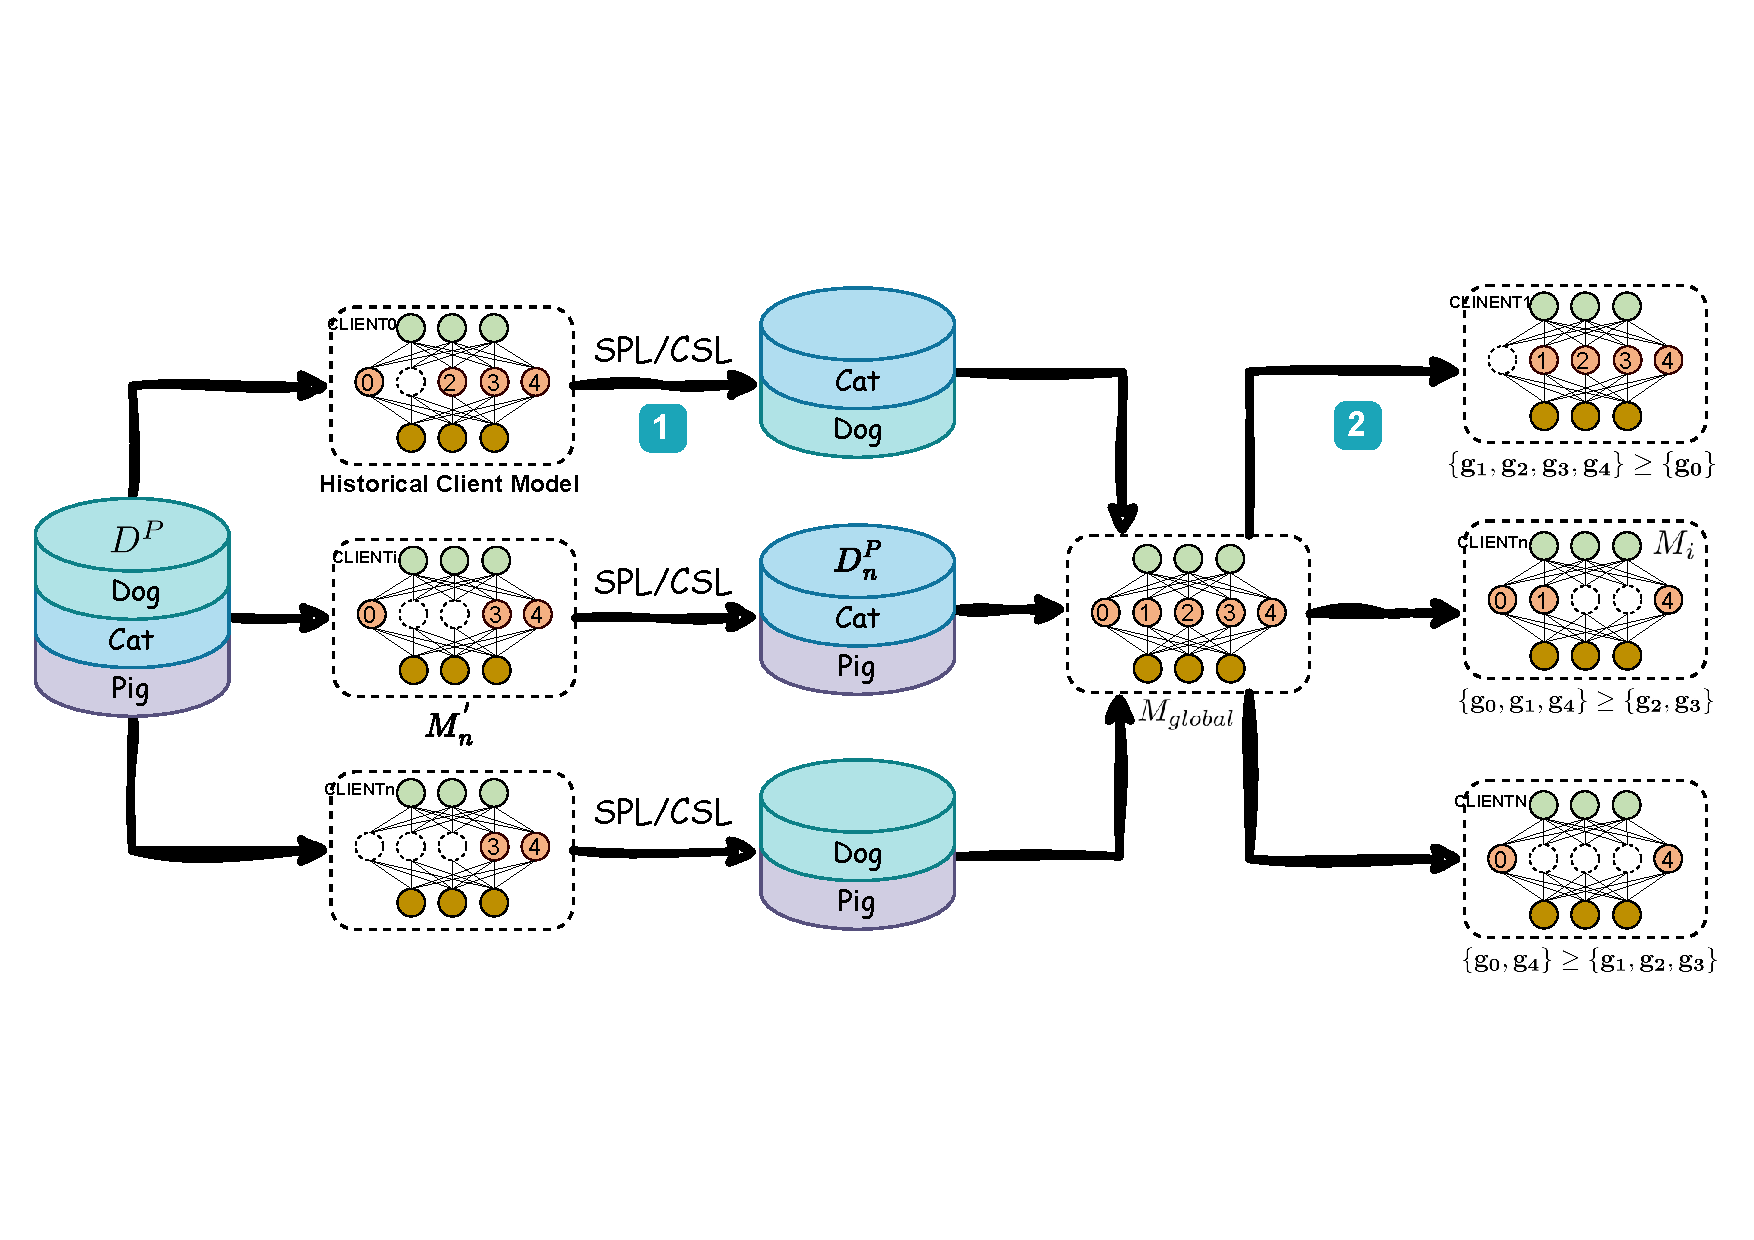
\includegraphics[width=0.9\linewidth]{chapter4/fedgseP.pdf}
    \caption{\label{fig:4-2overview}FedGSE算法中子模型抽取}
\end{figure}
%ppppppppppppppppppppppppppppppppppppppp
不同于FedDSE在客户端计算挑选,
FedGSE整个子模型计算挑选的过程都在中心侧服务器上进行。
算法\ref{alg:GetMaskFedDSE}详细描述了子模型抽取过程中生成
神经元掩码(mask)的过程。
首先在上一小章节中我们获得了相似数据集分布$\mathbb{D}_n^P$,
服务器将相似数据集分布输入到中心侧全局模型中,
经过反向传播获得整个全局模型所有神经元的梯度信息$\mathbf{g}$,
然后,服务器会从全局模型中逐层挑选神经元组成子模型。

我们将激活值的梯度的绝对值定义为每个神经元的梯度值。
具体来说,对于数据集$\mathbb{D}_n^P$中的每条数据
$(x, y)$(其中标签$y$可以是来自SPL真实标签或者是来自CSL伪标签),
第 $l$ 层第 $i$ 个神经元的激活值 $\mathbf{h}_{l,i}$的梯度是通过 
$\dfrac{\partial{f(\mathbf{w};x,y)}}{\partial{\mathbf{h}_{l,i}(k,v)}}$
来计算。
对于卷积神经网络来说,
其中第 $l$ 层第 $i$ 个神经元的激活值是一个特征图 $\mathbf{h}_{l,i} \in R^{K \times V}$,
其宽度为 $K$,长度为 $V$,我们使用平均值的绝对值来表示神经元梯度的大小:
\begin{equation}
    \label{eq:gradient}
    g_{l,i}=\sum_{k=0}^{K-1}\sum_{v=0}^{V-1}\Bigl| \sum_{(x,y)\in \mathbb{D}^P_n}\dfrac{\partial{f(\mathbf{w};x,y)}}{\partial{\mathbf{h}_{l,i}(k,v)}} \Bigr|
\end{equation}
使用等式 \ref{eq:gradient} 来定义神经元梯度主要有两个原因。
首先,现有的研究工作\cite{selvaraju2017grad}已经表明,
梯度较大的神经元更为重要,
这与我们挑选神经元的原则是一致的。
其次,在下一章节中,
我们会证明选择梯度较大的神经元会使得提取的子模型的梯度更接近全局完整模型。
%ccccccccccccccccccccccccccccccccccccccccccccccccccccccccccccccc
\begin{algorithm}[t]
    \caption{GetMaskFedGSE}
    \label{alg:GetMaskFedGSE}
    \begin{algorithmic}[1]
    \Require 客户端计$n$算能力系数 $r_n$,
            相似分布公共子数据集 $\mathbb{D}^P_n$, 
            中心侧全局模型 $\mathbf{w_{t}}$
    \Ensure 客户端$n$在$t$轮的掩码$\mathbf{M^{n,t}}$
    
    \Procedure{GetMask}{$r_n$, $\mathbb{D}^P_n$, $\mathbf{w_{t}}$}
        \State 使用公式\ref{eq:gradient}计算神经元梯度$\mathbf{g^n}$
        \For{对于每层 $l \in \{1,2, \cdots, L  \}$}
            \State $\mathbf{S}_{sorted} \leftarrow \textbf{sort}([g_{l,1}^n,\ldots, g_{l,m_l}^n])$
            \State $\mathbf{S}_{top-r} = \mathbf{S}_{sorted}[1 : r \cdot m_l]$
            
            \If{ $\mathbf{h_{l,i}} \in \mathbf{S}_{top-r}$}
            $\mathbf{M^{n,t}_{l,i}} = 1$
            \Else \text{ }$\mathbf{M^{n,t}_{l,i}} = 0$
            \EndIf
        \EndFor
        \State \Return $\mathbf{M^{n,t}}$
    \EndProcedure
    \end{algorithmic}
\end{algorithm}
%ccccccccccccccccccccccccccccccccccccccccccccccccccccccccccccccc

在每一层中,基于神经元梯度大小选择其中梯度绝对值相对较大的神经元。
与其他神经元相比,梯度绝对值较大的表示改变这些神经元
对模型最终的损失影响更大\cite{selvaraju2017grad},
也就意味着这些神经元更加重要。
我们规定客户端的计算能力系数为$r(0<r<1)$,
对于客户端n第 l 层,
我们仅保留该层中具有高梯度绝对值的$ r \cdot m_l$个神经元
(即 ${\max_{i=1}^{r \cdot m_l }}\{g_{l,1},g_{l,2},\dots,g_{l,m_l}\}$) ,
同时剪裁掉其他神经元。
我们在上述的挑选过程中产生一个不同神经元对应的二进制掩码$\mathbf{M}$,
挑选到的神经元在对象矩阵位置填写为$1$,
否则就是$0$,
例如,$\mathbf{M^n_{l,i}}=0$ 表示第 l 层的第 i 个神经元被剪除,
而 $\mathbf{M^n_{l,i}}=1 $ 表示保留该神经元。
根据这样的挑选规则也就是算法\ref{alg:GetMaskFedDSE}中所呈现的。
通过将全局模型参数与二进制掩码点乘法得到子模型参数,
客户端n的子模型参数为$\mathbf{w^n}=\mathbf{w} \odot \mathbf{M}$。



\subsection{端侧训练以及模型聚合}
FedGSE的整体工作流程如算法~\ref{alg:fedgse}所示。
在每一轮中,服务器首先为每个客户端建立数据集,
这些数据集的分布与它们各自的本地数据集相似(第6行),
然后为每个客户端提取子模型(第7-8行)。
之后,服务器将子模型发送给每个选中的客户端n(第9行)。
接着,每个客户端n使用其整个本地数据集对接收到的子模型进行本地训练(第16-18行)。
然后,每个客户端将其子模型的更新参数发送回服务器(第19行)。
最后,服务器聚合这些参数以更新全局模型(第11行),
更新与聚合方式详见FedDSE章节。


\section{理论分析}
在本节中,我们首先证明选择幅度较大的神经元梯度也等同于选择了重要的参数。
% {\CJKfamily{zhfsxt} 这是使用黑体显示的中文文本。} 
然后,我们证明FedGSE可以最大程度地减少子模型与完整全局模型之间的梯度差异。
\begin{lemma}\label{lm:1}
    参数的梯度与其对应激活值的梯度成正比,也即, 
    $\frac{\partial f(\mathbf{w})}{\partial \mathbf{w}_{l, i}} 
    =\mathbf{k} \cdot g_{l,i}$,
    其中$\mathbf{k}$是比例系数。
\end{lemma}
\underline{证明}:
我们考虑一个将ReLU作为激活函数,
\begin{equation}
    \label{eq:activatevalue}
    \mathbf{h}_{l,i} = \max  {\{ 0, \mathbf{w}_{l,i}^T \mathbf{h}_{l-1} + b_{l,i}  \}} 
\end{equation}
方程\ref{eq:activatevalue}表示具有ReLU激活函数的全连接。
然后我们可以得到
$\frac{\partial \mathbf{h}_{l,i}}{\partial \mathbf{w}_{l,i}} 
= \mathbf{h}_{l-1} \ or\  0 $
(除 $\mathbf{h}_{l-1}$ 使得 
$\mathbf{w}_{l,i}^T \mathbf{h}_{l-1} + b_{l,i}=0$,
因为$\frac{\partial \mathbf{h}_{l,i}}{\partial \mathbf{w}_{l,i}}$ 
在该点不可微
)。
\begin{equation}
    \label{eq:sgd}
     \frac{\partial f(\mathbf{w})}{\partial \mathbf{w}_{l, i}} = \frac{\partial f(\mathbf{w})}{\partial \mathbf{h}_{l,i}} \frac{\partial \mathbf{h}_{l,i}}{\partial \mathbf{w}_{l,i}}
  = \frac{\partial f(\mathbf{w})}{\partial \mathbf{h}_{l,i}} \mathbf{h}_{l-1}= g_{l,i} \mathbf{h}_{l-1}
\end{equation}
根据反向传播的链式法则和等式\ref{eq:activatevalue}的结论,
我们有  $\frac{\partial \mathbf{h}_{l,i}}{\partial \mathbf{w}_{l,i}}
 = \mathbf{h}_{l-1}$ 或者 $ 0 $。
很容易得出,参数的梯度与其对应激活值的梯度成正比(即引理 \ref{lm:1})。

引理\ref{lm:1}表明, 
$\frac{\partial f(\mathbf{w})}{\partial \mathbf{w}_{l,i}}$ 
和
$g_{l,i}$之间存在线性关系。
这意味着选择一个相对较大的$g_{l,i}$
等价于选择一个相对较大的
$\frac{\partial f(\mathbf{w})}{\partial \mathbf{w}_{l,i}}$。

\begin{theorem}\label{theorem:1} 
    考虑到 $\mathbb{D}^P_n$ 和客户端真实本地数据集 $\mathbb{D}_n$ 有着相近的分布,    
    从算法\ref{alg:GetMaskFedGSE}得到子模型参数$\mathbf{w}^n_*$
    与全局模型参数$\mathbf{w}$是最小的距离。
    具体来说,我们有
    \begin{align*}
        &  \Vert \nabla{f( \mathbf{w}; \mathbb{D}_n) } - \nabla{ f( \mathbf{w}^n; \mathbb{D}_n ) } \Vert \geq 
    \Vert \nabla{f( \mathbf{w}; \mathbb{D}_n) } - \nabla{ f( \mathbf{w}^n_*; \mathbb{D}_n ) } \Vert
    \end{align*}
    对于任何从全局模型 $\mathbf{w}$ 上抽取出来的子模型参数$\mathbf{w}^n$都成立, 
    % extracted from the global model $\mathbf{w}$ with the same size as 
    其中$\mathbf{w}^n$和$\mathbf{w}^n_*$拥有相同形状。
\end{theorem}
\underline{证明}:
我们的策略通过以下方式获得子模型的掩码$\mathbf{M}$ 
\begin{equation}
    \label{eq:getmask}
    \mathbf{M} = \textbf{GetMaskFedGSE}(r, \mathbb{D}^P_n , \mathbf{w})  %\textbf{\ \ Algorithm\  \ref{alg:GetMask} }
\end{equation}
其中 r 是客户端 n 的容量率。
然后,我们通过以下方式获得子模型参数 $\mathbf{w}^n_*$
\begin{equation}
    \label{eq:getw}
    \mathbf{w}^n_* = \mathbf{M} \odot \mathbf{w}
\end{equation}
我们考虑通过算法\ref{alg:GetMaskFedGSE}获得的子模型
$\mathbf{w}^n_*$
的第 l 层的梯度。
同时定义任意子模型
$\mathbf{w}^n$
的第 l 层的梯度
\begin{equation}
    \label{eq:wlist}
    \{\nabla{f(\mathbf{w}^n;\mathbb{D}^P_n)}\}_l = 
    \{ \overbrace{g_1^n, \dots , g_{r \cdot m_l}^n}^{r \cdot m_l }, 
    \overbrace{0, \dots, 0}^{(1-r) \cdot m_l}  \}
\end{equation}

\begin{equation}
    \label{eq:wlist*}
    \{\nabla{f(\mathbf{w}^n_*;\mathbb{D}^P_n)}\}_l = 
    \{ \overbrace{g_1^*, \dots , g_{r \cdot m_l}^*}^{r \cdot m_l }, 
    \overbrace{0, \dots, 0}^{(1-r) \cdot m_l}  \}
\end{equation}
其中 $m_l$ 是第 $l$ 层神经元的总数。
其中有$r \cdot m_l$个神经元的梯度非零,
$(1-r) \cdot m_l$ 个神经元的梯度为零。
不失一般性,
我们假设等式(\ref{eq:wlist})是按降序排列的,
也就是
$g_1 \geq g_2 \geq \dots \geq g_{r \cdot m_l} \geq 0$,
等式(\ref{eq:wlist*})也是同样的顺序。

根据等式(\ref{eq:getmask})和等式(\ref{eq:getw}),
我们可以得到 
$ g_1^* \geq g_1^n , \dots , g_{r \cdot m_l}^* \geq g_{r \cdot m_l}^n $,
这是因为FedGSE就是挑选其中神经元梯度大组成子模型的。
然后,很明显可以得出,
\begin{equation}
    \label{eq:layergeq}
    \sum_{i=0}^{m_l}|g_{l,i}-g_{l,i}^n| \geq 
    \sum_{i=0}^{m_l}|g_{l,i}-g_{l,i}^*|
\end{equation}
其中$g_{l,i}$是全局模型$\mathbf{w}$ 在第 l 层的第 i 个神经元的梯度。
当第 i 个神经元被剪枝后,
$g_{l,i}^n$ 和 $g_{l,i}^*$ 都按照 0 处理。
等式(\ref{eq:layergeq})表明,对于每一层,
$\mathbf{w}$ 和 $\mathbf{w}^n$
之间的梯度差异小于
$\mathbf{w}$ 和 $\mathbf{w}^n$。
因此,在总结所有层时,我们可以得出以下结论:
\begin{equation}\label{eq:SimilarGradient}
    \Vert \nabla{f( \mathbf{w}; \mathbb{D}^P_n) } - \nabla{ f( \mathbf{w}^n; \mathbb{D}^P_n ) } \Vert \geq 
  \Vert \nabla{f( \mathbf{w}; \mathbb{D}^P_n) } - \nabla{ f( \mathbf{w}^n_*; \mathbb{D}^P_n ) } \Vert
\end{equation}
根据等式(\ref{eq:sameDataDis}),
$\mathbb{D}^P_n$ 与 $\mathbb{D}_n$ 相似,
我们可以通过在等式(\ref{eq:SimilarGradient})中将
$\mathbb{D}^P_n$ 替换为 $\mathbb{D}_n$
来推导出定理 \ref{theorem:1}。

定理 \ref{theorem:1}证明了使用由我们的算法\ref{alg:fedgse}
所选的子模型在本地数据集上进行模型更新,
可以最小化使用子模型进行本地更新与使用原始全局模型进行本地更新之间的差异。

\section{实验过程与结果分析}
本章节解决的问题是章节 \ref{sec:chapterfeddse}的改进和提升,
因此大部分的实验设定与章节 \ref{sec:chapterfeddse}应用同样设定。
但是两种改进方法适用于不同的场景,
% FedDSE需要再客户端上前向传播然后在客户端上进行子模型抽取的工作,
FedDSE方法主要解决在低质量客户端分布的场景下,
指的是所有的客户端都不能训练中心侧全局模型。
而FedGSE方法则是应用在高质量客户端分布场景下,
在这种场景下客户端中分布着一部分可以训练中心侧的模型,
本章节的实验结果均是在这种场景下进行的。

\begin{table}[thbp]
    \caption{\label{tab:train_fedgse_info}FedGSE不同数据集训练参数设置}
    \begin{tabularx}{\linewidth}{l X<{\centering} X<{\centering} X<{\centering} X<{\centering}}
        \toprule
        & EMNIST & CIFAR-10 & CIFAR-100 & TinyImageNet \\ \hline
        本地训练次数(E) & $2$ & $2$ & $2$ & $2$ \\ 
        学习率 & $0.001$ & $0.001$ & $0.001$ & $0.001$ \\ 
        训练轮次 & $800$ & $2500$ & $2500$ & $2500$ \\ 
        优化器 & SGD & SGD & SGD & SGD \\ 
        动量 & $0.9$ & $0.9$ & $0.9$ & $0.9$ \\ 
        权重衰减 & $5.00\text{E}-04$ & $5.00\text{E}-04$ & $5.00\text{E}-04$ & $5.00\text{E}-04$ \\ 
        相似数据量 & 128 & 128 & 128 & 128 \\ 
        \bottomrule
    \end{tabularx}
\end{table}
与在FedDSE上一样,
我们在数据集EMNIST上训练四层卷积神经网络,
同样,
使用Resnet18处理数据集CIFAR10和CIFAR100
以及
使用Resnet34处理数据集TinyImagenet,
详见章节\ref{sec:feddsedata_model}。
对于实验设置中的数据异质性还是分为
高数据异质性与低数据异质性,
参见表\ref{tab:classinfo}。
而FedGSE的模型异质性则是在高质量客户端分布场景,
具体来讲就是设定五种客户端计算资源分别是
$\mathbf{r} = \{ 1, 0.5, 0.25, 0.125, 0.0625 \}$,
与上一章节不同的是本章节实验中包含了百分之二十比例的可以
训练中心侧全局模型的客户端,
表\ref{tab:paraAndmac}展示了不同抽取方法中不同模型
平均的参数量级和MACs。
我们对比的baseline与FedDSE是一致的,
也即HeteroFL、FedRolex、Federated Dropout和DepthFL。
表\ref{tab:train_fedgse_info}中详细描述了本章节实验所设定的参数,
其中大部分的设定与FedDSE一致,
但是最后一行相似数据表示输入在
中心侧模型中用于反向传播梯度的数据量。
整个训练过程在PyTorch框架上进行,
本章节实验所用的设备是Nvidia 4090。
最后因为实验是关于分类问题,
评估指标选择的是在整个测试集上模型准确率。
在训练过程中,
我们采取了与章节\ref{sec:feddse_tricks}中一致的策略,
掩码交叉熵损失、放缩模块以及静态批归一化。
以上是本章节实验的所有设置以及详细介绍与
FedDSE相似以及存在区别的地方。
\begin{table}[thbp]
    \caption{\label{tab:paraAndmac}不同抽取方法平均模型参数量/MACs}
    \begin{tabularx}{\linewidth}{l  X<{\centering} X<{\centering} X<{\centering}}
        \toprule
        抽取方法 & CONV & ResNet18 & ResNet34  \\ \hline
        DepthFL &  1319k/35.80M &  4.48M/378.7M  & 8.54M/745.37M  \\ 
        others & 441.19k/16.12M  & 3.08M/155.12M &  5.9M/331.57M  \\ 
        \bottomrule
    \end{tabularx}
\end{table}


\subsection{实验结果}

\begin{table}[thbp]
    \caption{\label{tab:feddse_total_high_res}高质量客户端分布场景中低数据异质性下不同方法准确率对比}
    \begin{tabularx}{\linewidth}{l X<{\centering} X<{\centering} X<{\centering} X<{\centering}}
        \toprule
        方法 & EMNIST & CIFAR-10 & CIFAR-100 & TinyImageNet \\ \hline
        HeteroFL & 96.11 & 56.08 & 25.95 & 21.82 \\ 
        Federated Dropout & 88.76 & 52.57 & 15.79 & 19.25 \\ 
        FedRolex & 93.94 & 57.28 & 21.53 & 22.96 \\ 
        DepthFL & 97.69 & 63.90 & 31.38 & 24.85 \\ 
        FedGSE\_CSL & \textbf{98.06}  & \textbf{65.89} & \textbf{31.46} & \textbf{25.95}  \\ 
        FedDSE\_SPL & 97.44  & 65.82 & 28.87 &  25.33 \\ 
        \bottomrule
    \end{tabularx}
\end{table}


\begin{table}[thbp]
    \caption{\label{tab:feddse_total_low_res}高质量客户端分布场景中低数据异质性下不同方法准确率对比}
    \begin{tabularx}{\linewidth}{l X<{\centering} X<{\centering} X<{\centering} X<{\centering}}
        \toprule
        方法 & EMNIST & CIFAR-10 & CIFAR-100 & TinyImageNet \\ \hline
        HeteroFL & 98.65 & 73.42 & 32.13 & 29.56 \\ 
        Federated Dropout & 97.53 & 65.28 & 19.81 & 26.04 \\ 
        FedRolex & 98.56 & 71.68 & 27.60 & 30.01 \\ 
        DepthFL & \textbf{99.14} & \textbf{76.13} & \textbf{33.24} & 29.83 \\ 
        FedGSE-CSL & 98.74 & 73.51  & 32.65 & 30.02  \\ 
        FedDSE-SPL & 98.77 & 74.66  & 32.40 &\textbf{30.49} \\ 
        \bottomrule
    \end{tabularx}
\end{table}
表\ref{tab:feddse_total_high_res}与表\ref{tab:feddse_total_low_res}
展示了我们在相同实验设置下执行的实验结果,
以确保公平性。
结果表明,我们的方法FedGSE相比于其他方法中表现更优,
特别是在高数据异质性情况下,
相较于HeteroFL、Federated Dropout和FedRolex在EMNIST、
CIFAR10、CIFAR100和TinyImageNet上的最佳表现,
分别提升了
$1.33\%$, $8.54\%$, $2.92\%$ 和 $2.37\%$。
此外,我们的方法在低数据异质性情况下也表现出色,
相较于其他三种方法的最佳表现
分别有$0.12\%$, $1.24\%$, $0.27\%$ 和 $0.39\%$ 
的提升。
上述现象表明,
我们的方法在高数据异质性情况下具有显著优势,
这验证了我们的理论,即数据异质性越高,
我们的方法越能有效选择重要神经元来建模这些数据。
Federated Dropout在大多数场景中表现相对较差,
主要是因为其动态选择神经元的机制。
对于简单的数据集EMNIST,我们的方法与其他方法在准确率上的差异较小,
无论是在高还是低数据异质性情况下,这是因为CNN模型很容易训练EMNIST,
因此所有方法都能获得相对较好的结果。
对于CIFAR10,
FedGSE展示了其在算法设计上的优越性,
相较于FedRolex分别有$8.54\%$ 和 $2.98\%$ 的优势。
随着数据异质性的降低,
优势有所缩小,但仍保持领先。
尽管在困难的数据集CIFAR-100和TinyImageNet上,
所有方法的表现都不如其他数据集,但我们的方法仍然领先于其他方法。
总体而言,
FedGSE在低数据异质性和更具挑战性的高数据异质性场景下均优于HeteroFL、
Federated Dropout和FedRolex,特别是在高数据异质性情况下。
尽管DepthFL根据表\ref{tab:paraAndmac}具有更大的参数和MACs,
但在高数据异质性情况下的表现仍不如FedGSE,
但在低数据异质性情况下,DepthFL取得了一定的优势。

\subsection{对比FedGSE-CSL与FedDSE-SPL}
FedGSE-CSL与FedGSE-SPL的核心区别在于获取相似分布数据的方法,
FedGSE-CSL使用的是客户模型设定无标签数据集(CSL),
而FedGSE-SPL使用的是服务器侧挑选有标签数据集(SPL)。
在高数据异质性的情况下,FedDSE-SPL 无法达到 FedGSE-CSL 的水平。
由于客户端上传的模型是基于本地数据集进行训练的,
而本地数据集包含的类别数量较少(例如,在EMNIST和CIFAR10中,类别数量为2),
因此FedDSE-SPL难以选择所有应该被选中的数据。
然而,在低数据异质性的情况下,客户端数据集包含的类别数量更多,
如表\ref{tab:classinfo}所示。
这提供了一种具有鲁棒性容忍度的方法,
即少量预测错误不会影响整体神经元选择。
相比之下,
FedGSE-CSL的错误标签对其准确性下降起到了显著作用。

\subsection{累积梯度差异分析}
我们设计了在EMNIST数据集上使用简单卷积神经网络的实验,
以分析不同训练轮次中的累积梯度差异。
实验的目的是确定全局模型参数与子模型参数之和之间的差异。
在同一轮次中使用相同的本地数据进行训练后,
计算全局模型与子模型之间更新参数的差异。
%ppppppppppppppppppppppppppppppppppppppp
\begin{figure}[thbp]
    \centering
    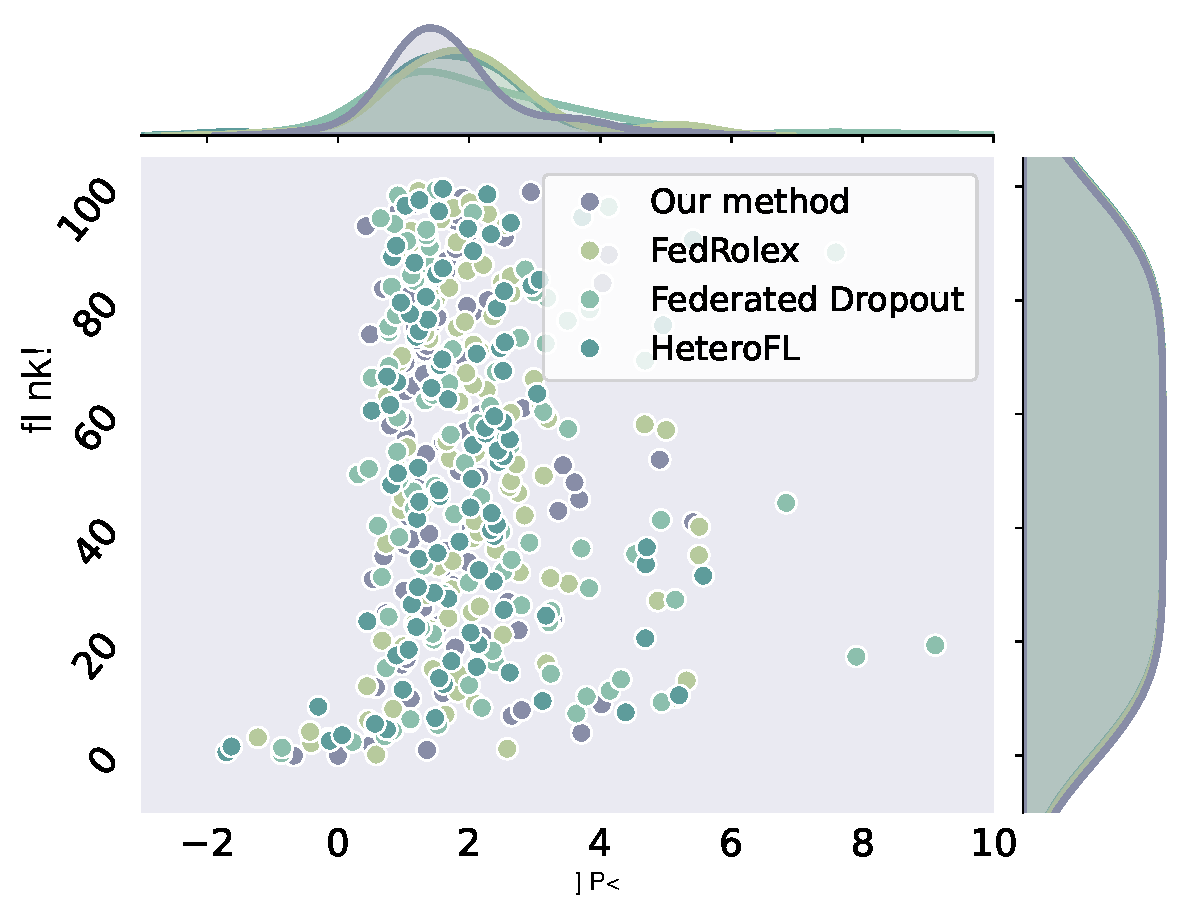
\includegraphics[width=0.95\linewidth]{chapter4/difference_fedgse1.pdf}
    \caption{\label{fig:4-4fedgse_difference}不同通讯轮次全局模型与子模型梯度差值}
\end{figure}
%ppppppppppppppppppppppppppppppppppppppp
在图\ref{fig:4-4fedgse_difference}中,
纵坐标的值表示的是通讯轮次,
本次实验总共设定了100个通讯轮次,
横坐标表示的是差值,
也就是子模型的梯度总和与全局模型梯度总和的差值。
上方的曲线图表示的是在所有轮次中统计的差值出现的次数的曲线图。
通过曲线图可以发现FedGSE-CSL方法峰值更偏向于0附近
也就是差值集中在较小的值附近,
相比于其他方法更为明显,
峰值明显往右边偏移,
这就意味着在整个训练的100个轮次中,
整体差值FedGSE-CSL是远远小于其他方法的。


% \begin{figure}[thbp]
%     \centering
%     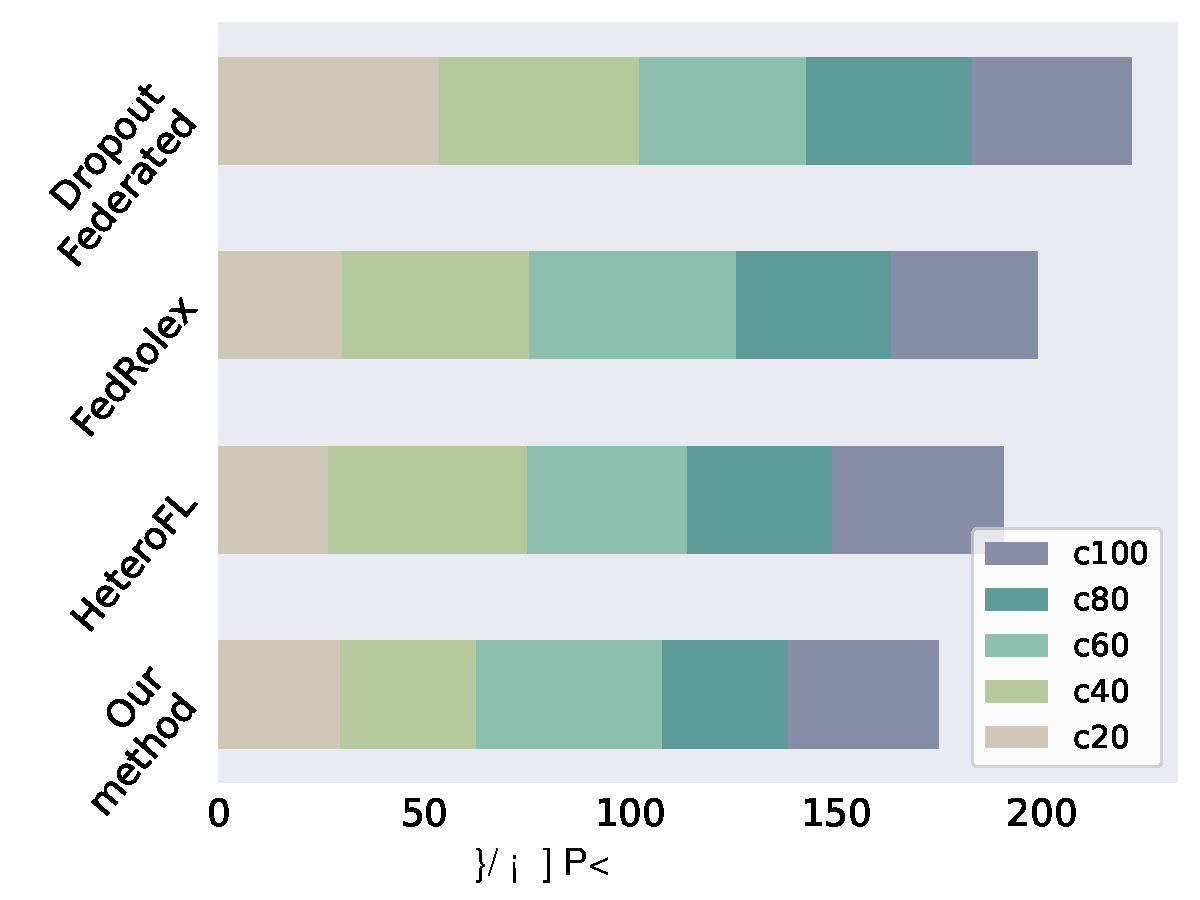
\includegraphics[width=0.9\linewidth]{chapter4/acc_distance_histogram.pdf}
%     \caption{\label{fig:4-4fedgse_acc_difference}特定通讯轮次下累计梯度差值}
% \end{figure}
%ppppppppppppppppppppppppppppppppppppppp
\begin{figure}[thbp]
    \centering
    \subfloat[特定通讯轮次下累计梯度差值]{%
        \begin{minipage}{0.48\textwidth}
        \centering
        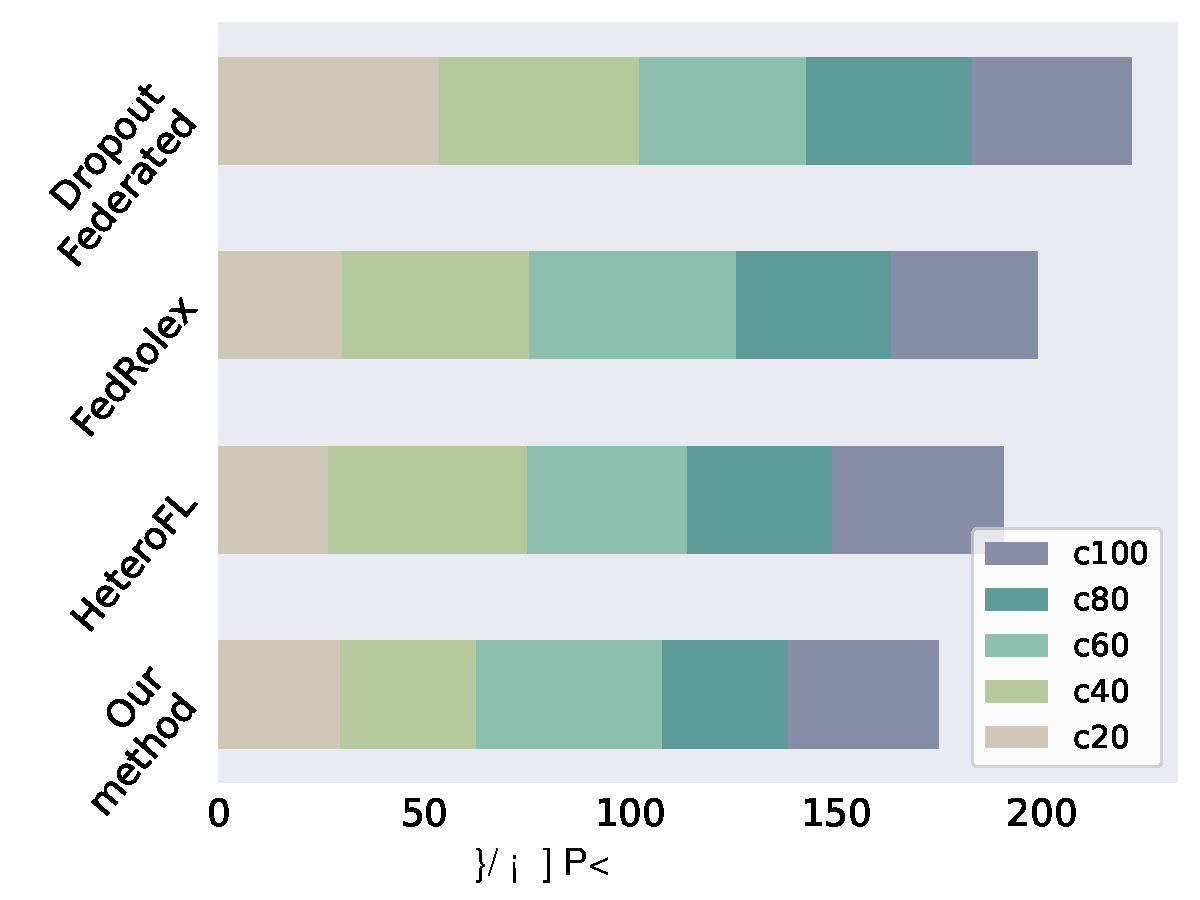
\includegraphics[width=\textwidth]{chapter4/acc_distance_histogram.pdf}
        \label{fig:4-4fedgse_acc_difference}
        \end{minipage}
    }
    \hfill
    \subfloat[EMNIST不同方法的准确率]{%
        \begin{minipage}{0.48\textwidth}
        \centering
        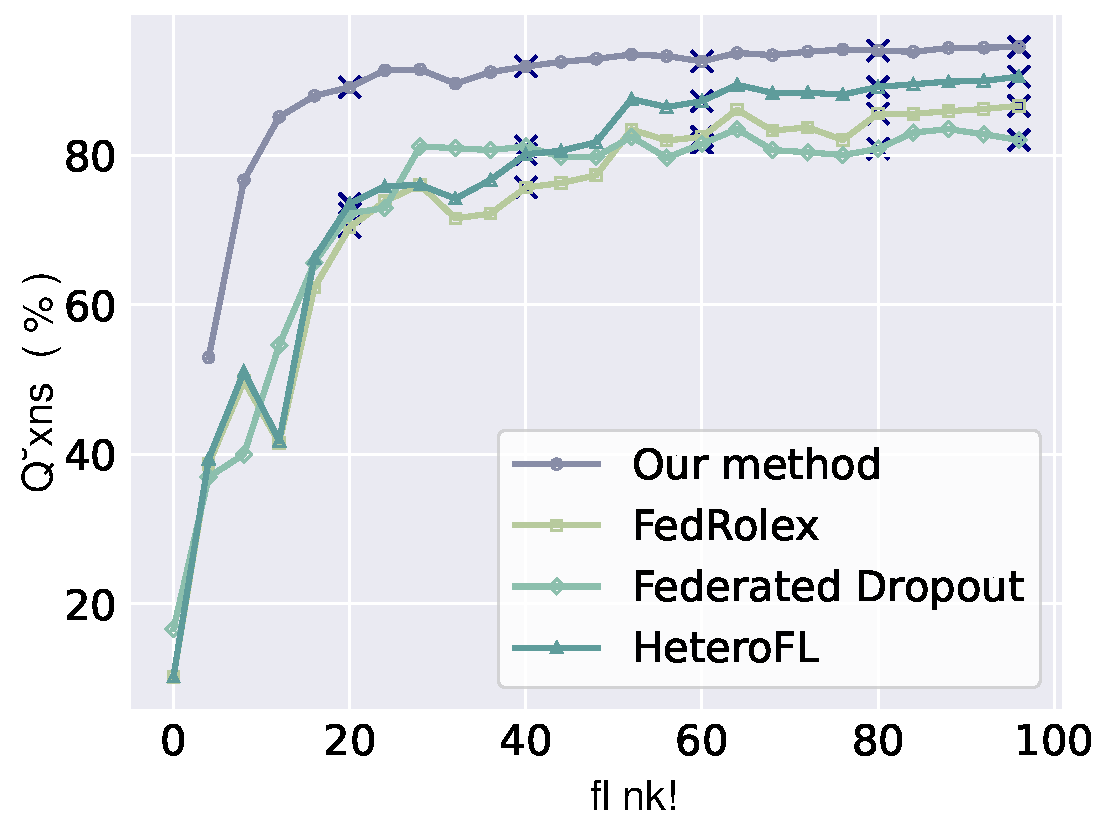
\includegraphics[width=\textwidth]{chapter4/acc-acc.pdf}
        \label{fig:emnist_accuracy}
        \end{minipage}
    }
    \hfill
    % \vspace{-0.5cm}
    \caption{累计误差与准确率关系}
    \label{fig:dis_all1}
    % \vspace{-0.5cm}
\end{figure}
% ppppppppppppppppppppppppppppppppppppppp


具体来说,我们对通信轮次
$\{ 20, 40, 60, 80, 100 \}$ 
中的累积误差(\textbf{A}ccumulated \textbf{D}ifferences AD)进行了统计分析,
也就是计算前20、40、 60 、 80 以及100轮次之前的所有轮次误差的总和,
结果如图\ref{fig:4-4fedgse_acc_difference}所示。
其中纵坐标表示不同方法,
而横坐标表示的是具体的差值数据。
可以明显观察到,在每一个统计轮次中,累计误差的大小关系均为
$\{ Ad_{Federated Dropout} > Ad_{FedRolex} > Ad_{HeteroFL} > Ad_{FedGSE} \}$, 
这表明FedGSE-CSL有效地缩小了全局模型与子模型之间的更新梯度参数差距距离。
可以使得客户端朝最优方向训练。
根据图\ref{fig:emnist_accuracy},准确率的结果为
$\{ Acc_{Federated Dropout} < Acc_{FedRolex} < Acc_{HeteroFL} < Acc_{FedGSE} \}$ ,
这与累积误差的恰好结果相反。
毫无疑问可以合理推断出较小的累积误差往往可以得到更高的准确率。

\section{消融实验}
\subsection{客户端计算能力分布对模型能力的影响}
在之前的实验中,客户端的容量是均匀设置的。
为了探究客户端模型异质性分布的影响,
在高客户端质量分布的情况下,
我们选择了容量$\{1, \frac{1}{16} \} $(低客户质量分布中没有1),
并调整了两者之间的分布比例(定义为$\rho$),
其中$\rho=1$表示所有客户端都具有最大容量模型为 $\{1 \} $的情况,
而$\rho=0$ 表示所有客户端都具有最小容量模型为 $\{ \frac{1}{16} \} $的情况。


\textbf{FedGSE下高数据异质性和低数据异质性的对比分析 }
\begin{figure}[thbp]
    \centering
    \subfloat[EMNIST下高数据异质]{%
        \begin{minipage}{0.48\textwidth}
        \centering
        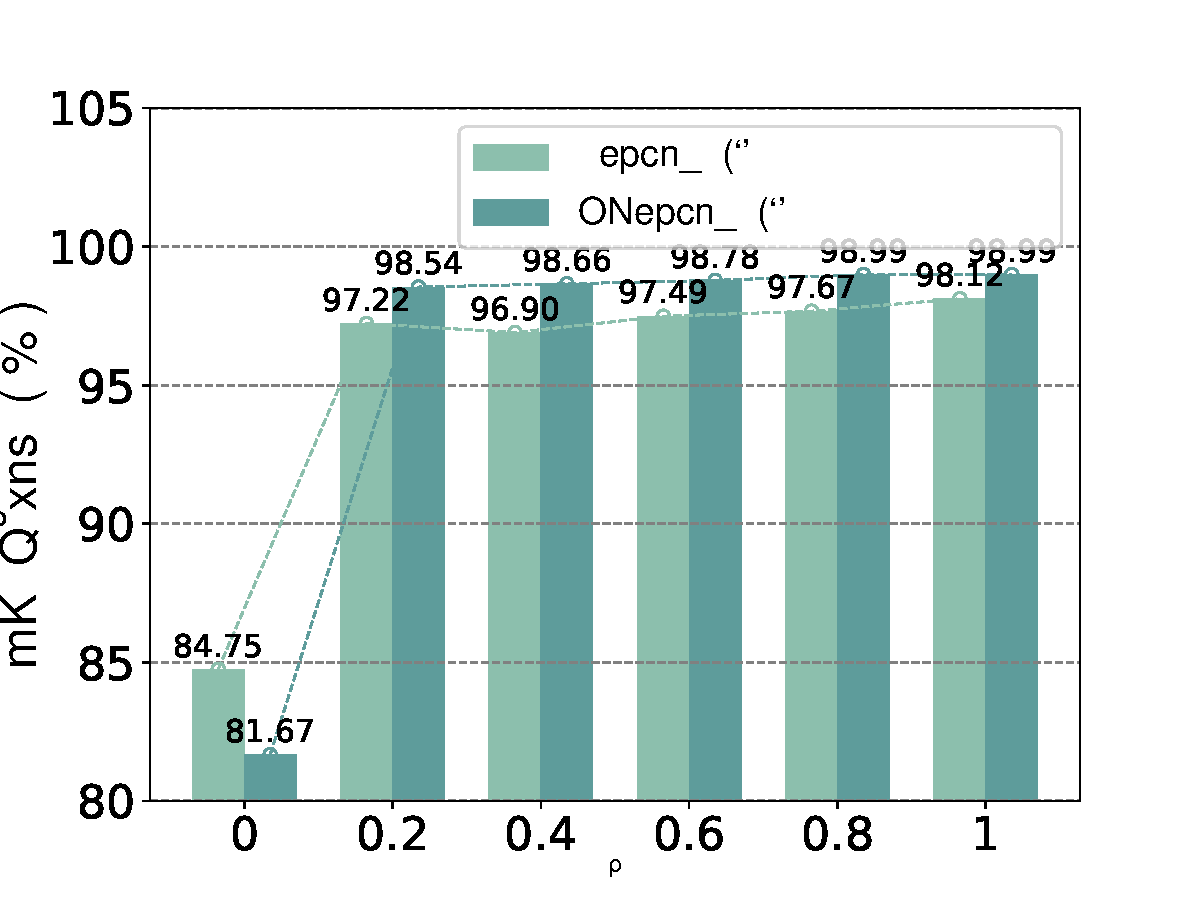
\includegraphics[width=\textwidth]{chapter4/dis_emnist.pdf}
        \label{fig:dis_emnist}
        \end{minipage}
    }
    \hfill
    \subfloat[EMNIST下低数据异质]{%
        \begin{minipage}{0.48\textwidth}
        \centering
        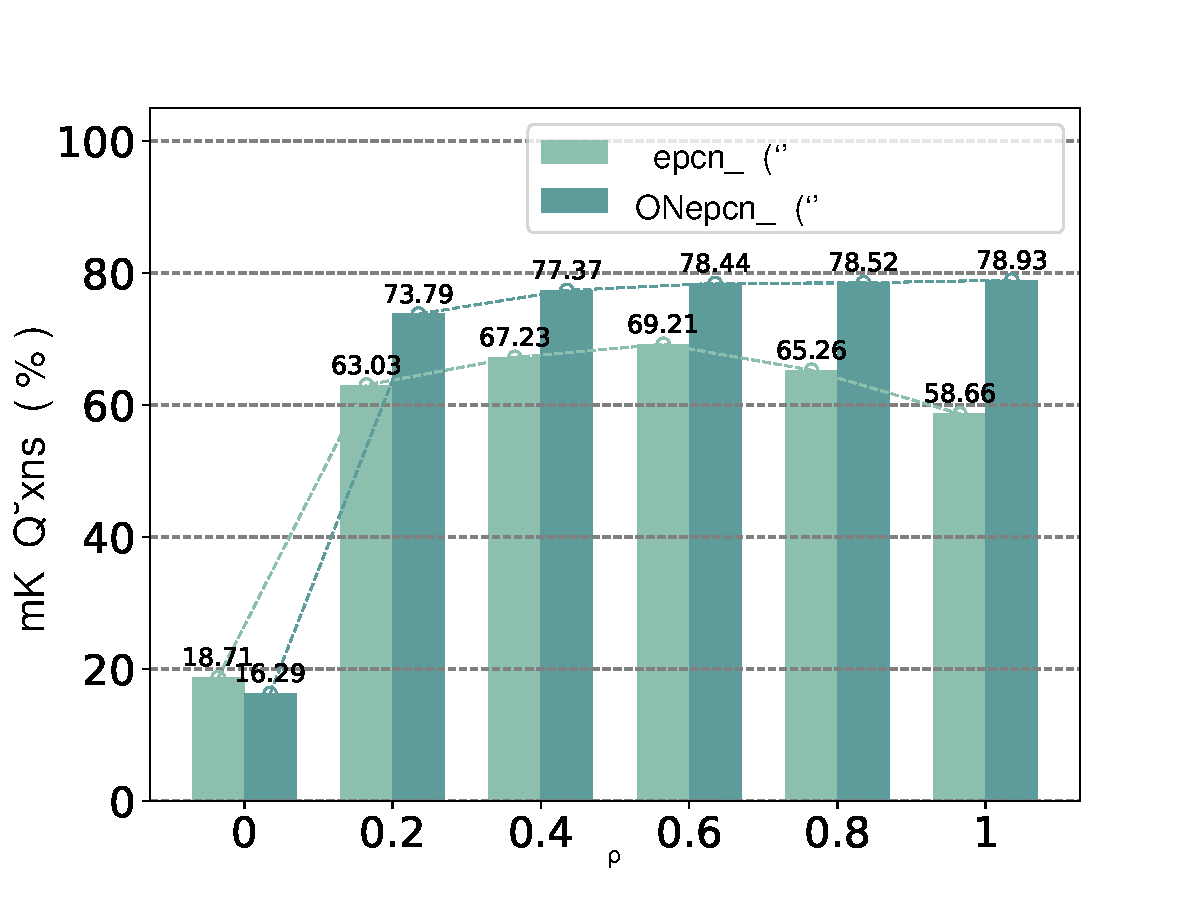
\includegraphics[width=\textwidth]{chapter4/dis_cifar.pdf}
        \label{fig:dis_cifar}
        \end{minipage}
    }
    \hfill
    % \vspace{-0.5cm}
    \caption{FedGSE下高数据异质性和低数据异质性的对比分析}
    \label{fig:dis_all}
    % \vspace{-0.5cm}
\end{figure}
图\ref{fig:dis_emnist}和图\ref{fig:dis_cifar}展示了在EMNIST和CIFAR10数据集上,
当$\rho$从0变化到1时,
使用我们的方法时全局模型的变化情况。我们可以观察到:
(1)当$\rho$从0到0.2时,
无论是在高数据异质性还是低数据异质性下,
EMNIST和CIFAR10的全局模型准确率都经历了一个显著的提升。
这表明模型规模是导致上述情况的主要原因。
\begin{figure}[thbp]
    \centering
    \subfloat[EMNIST下高数据异质]{%
        \begin{minipage}{0.48\textwidth}
        \centering
        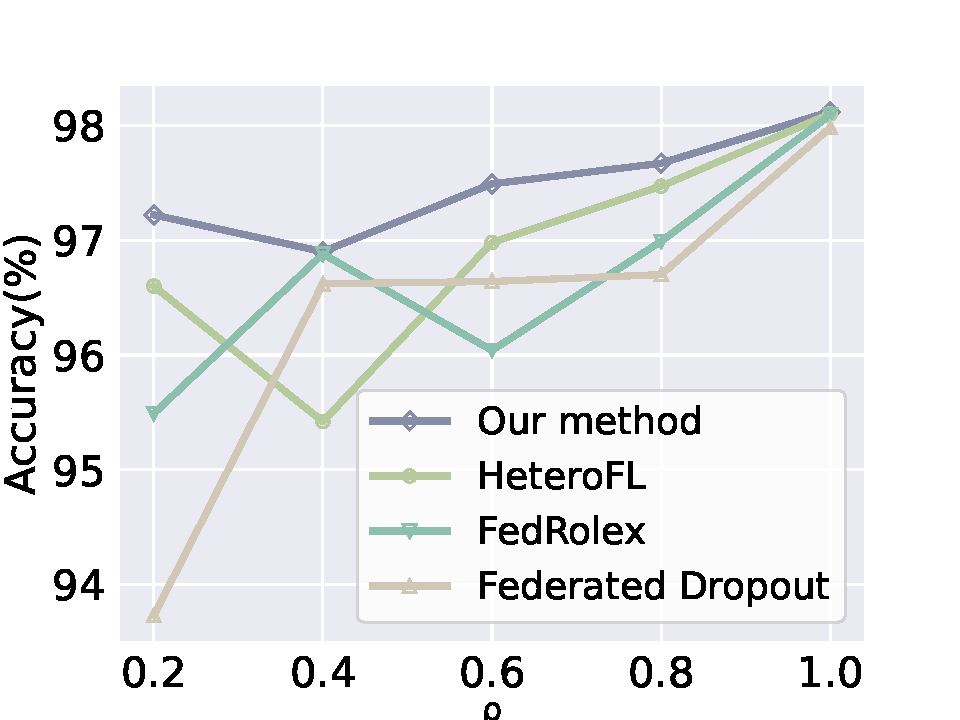
\includegraphics[width=\textwidth]{chapter4/high_probs_acc_emnist.pdf}
        \label{fig:comp-emnist-high}
        \end{minipage}
    }
    \hfill
    \subfloat[EMNIST下低数据异质]{%
        \begin{minipage}{0.48\textwidth}
        \centering
        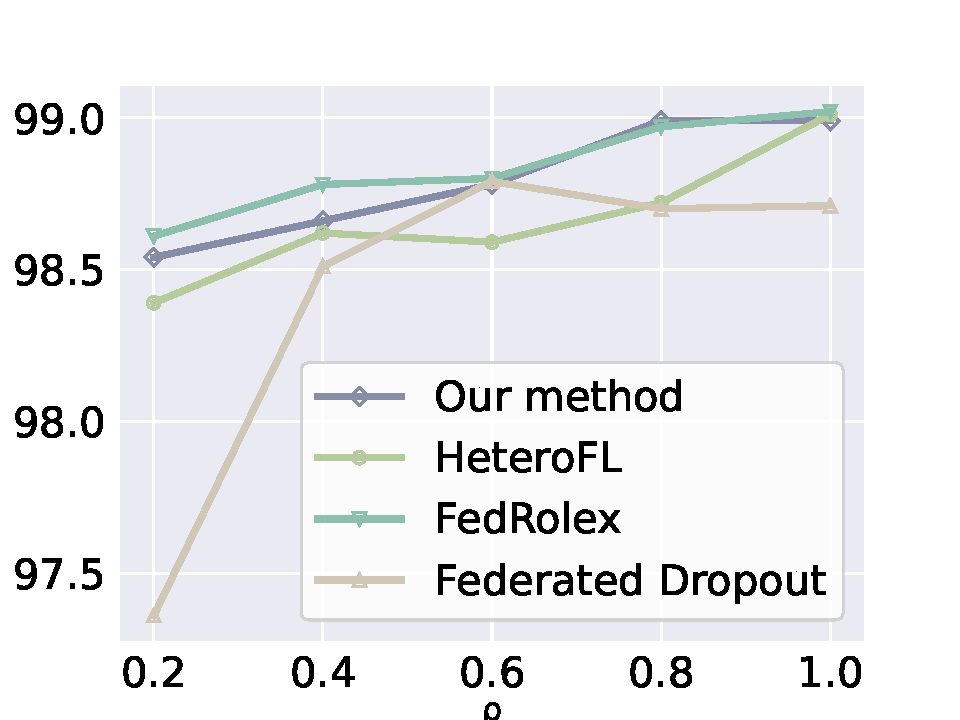
\includegraphics[width=\textwidth]{chapter4/low_probs_acc_emnist.pdf}
        \label{fig:comp-emnist-low}
        \end{minipage}
    }
    \hfill
    % \vspace{-0.5cm}
    \caption{ EMNIST 上$\rho$对准确率影响曲线图}
    \label{fig:motivation_distribution_emnist}
    % \vspace{-0.5cm}
\end{figure}
(2)对于简单的数据集EMNIST,
在$\rho$的广泛范围内(从0到1),
高数据异质性和低数据异质性之间的全局准确率存在差距。
这是因为EMNIST是一个简单的任务,
四层卷积神经网络模型可以轻松达到85\%的全局模型准确率。
因此,全局模型准确率受到数据异质性水平的限制,而不是模型容量。
这一结果揭示了数据异质性的挑战无法通过增加模型容量来解决。
\begin{figure}[thbp]
    \centering
    \subfloat[EMNIST下高数据异质]{%
        \begin{minipage}{0.48\textwidth}
        \centering
        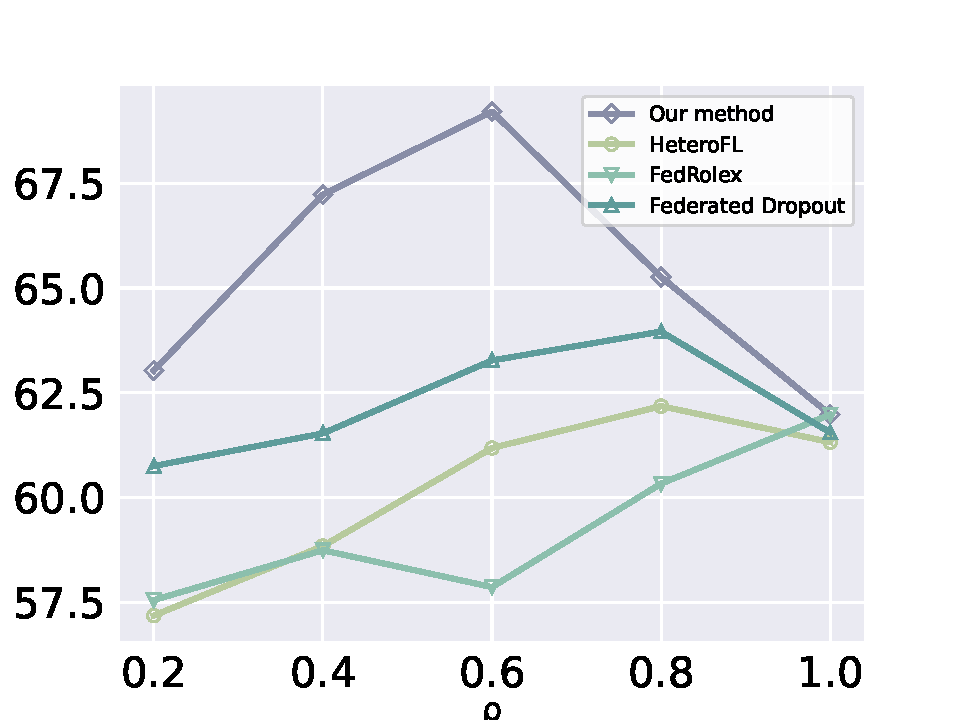
\includegraphics[width=\textwidth]{chapter4/high_probs_acc_cifar10.pdf}
        \label{fig:comp-cifar-high}
        \end{minipage}
    }
    \hfill
    \subfloat[EMNIST下低数据异质]{%
        \begin{minipage}{0.48\textwidth}
        \centering
        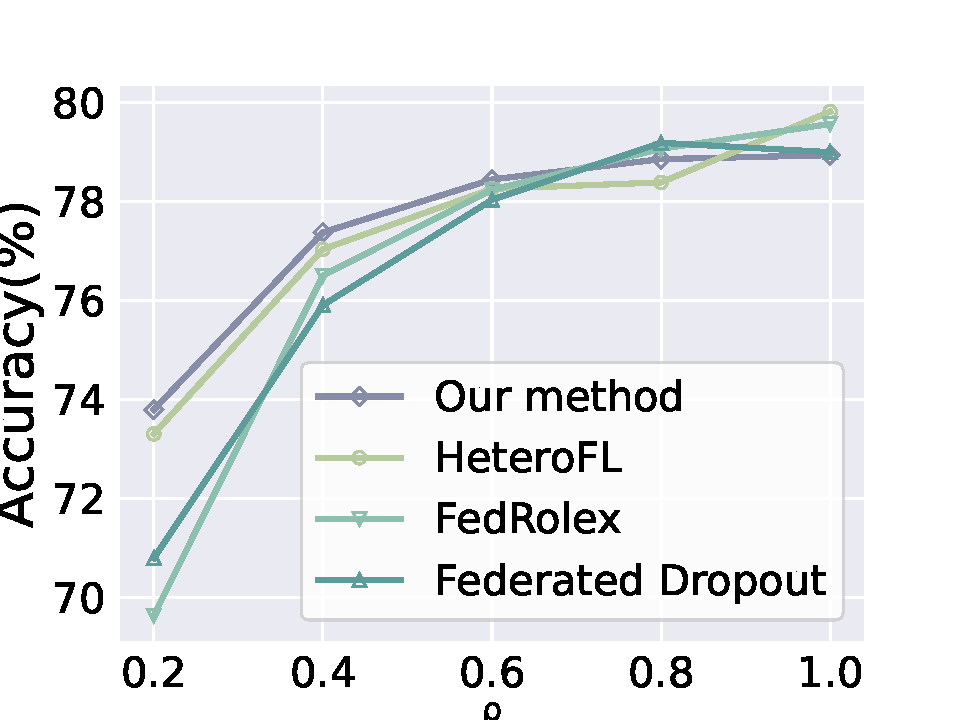
\includegraphics[width=\textwidth]{chapter4/low_probs_acc_cifar10.pdf}
        \label{fig:comp-cifar-low}
        \end{minipage}
    }
    \hfill
    % \vspace{-0.5cm}
    \caption{ CIAFR10 上$\rho$对准确率影响曲线图}
    \label{fig:motivation_distribution_cifar}
    % \vspace{-0.5cm}
\end{figure}
(3)对于CIFAR10,高数据异质性和低数据异质性之间的全局准确率存在较大差距。
全局模型准确率受到模型最大容量和数据异质性水平的限制。
具有
$\frac{1}{16}$
容量的客户端模型根本无法解决此类问题,导致准确率极低。这导致了较大的差距。

\textbf{不同方法的对比分析 }
如图\ref{fig:comp-emnist-high}和图\ref{fig:comp-cifar-high}所示,
在高数据异质性场景下,我们的方法在整个$\rho$从0.2到1的变化过程中,
相较于其他方法具有压倒性的优势。
这表明,增加模型的能力并不一定能够提高全局准确率,
而在高数据异质性场景下,良好的算法设计可以提升模型的准确率。
在困难场景下,我们的方法远远超过了其他模型,证明了我们的算法在这种情况下的优势。
而在低数据异质性场景下,
如图\ref{fig:comp-emnist-low}和图\ref{fig:comp-cifar-low}所示,
我们的方法在大多数情况下表现良好。
在这种简单场景下,大多数方法都能取得良好的结果,
这表明在当前场景下,全局准确率的限制主要来自于模型的能力,
提升模型的能力可以提高效果。
特别是在图\ref{fig:comp-cifar-high}中,
在具有高数据异质性的困难数据集上,增加模型的能力并不能稳定地提高模型的准确率。
综上所述,在针对高数据异质性的严格场景中,
我们的方法比其他方法更具适用性。
图\ref{fig:emnist-high-high}
展示了在EMNIST数据集上的特殊训练过程,
可以看到在大多数的训练过程中,
我们的方法全程都优于其他的方法,
在少部分中处于焦灼的状态。

\begin{figure}[thbp]
    \subfloat[$\rho=0.2$]{
    \begin{minipage}{0.42\textwidth}
    \label{fig:emnist-high-0.2}
    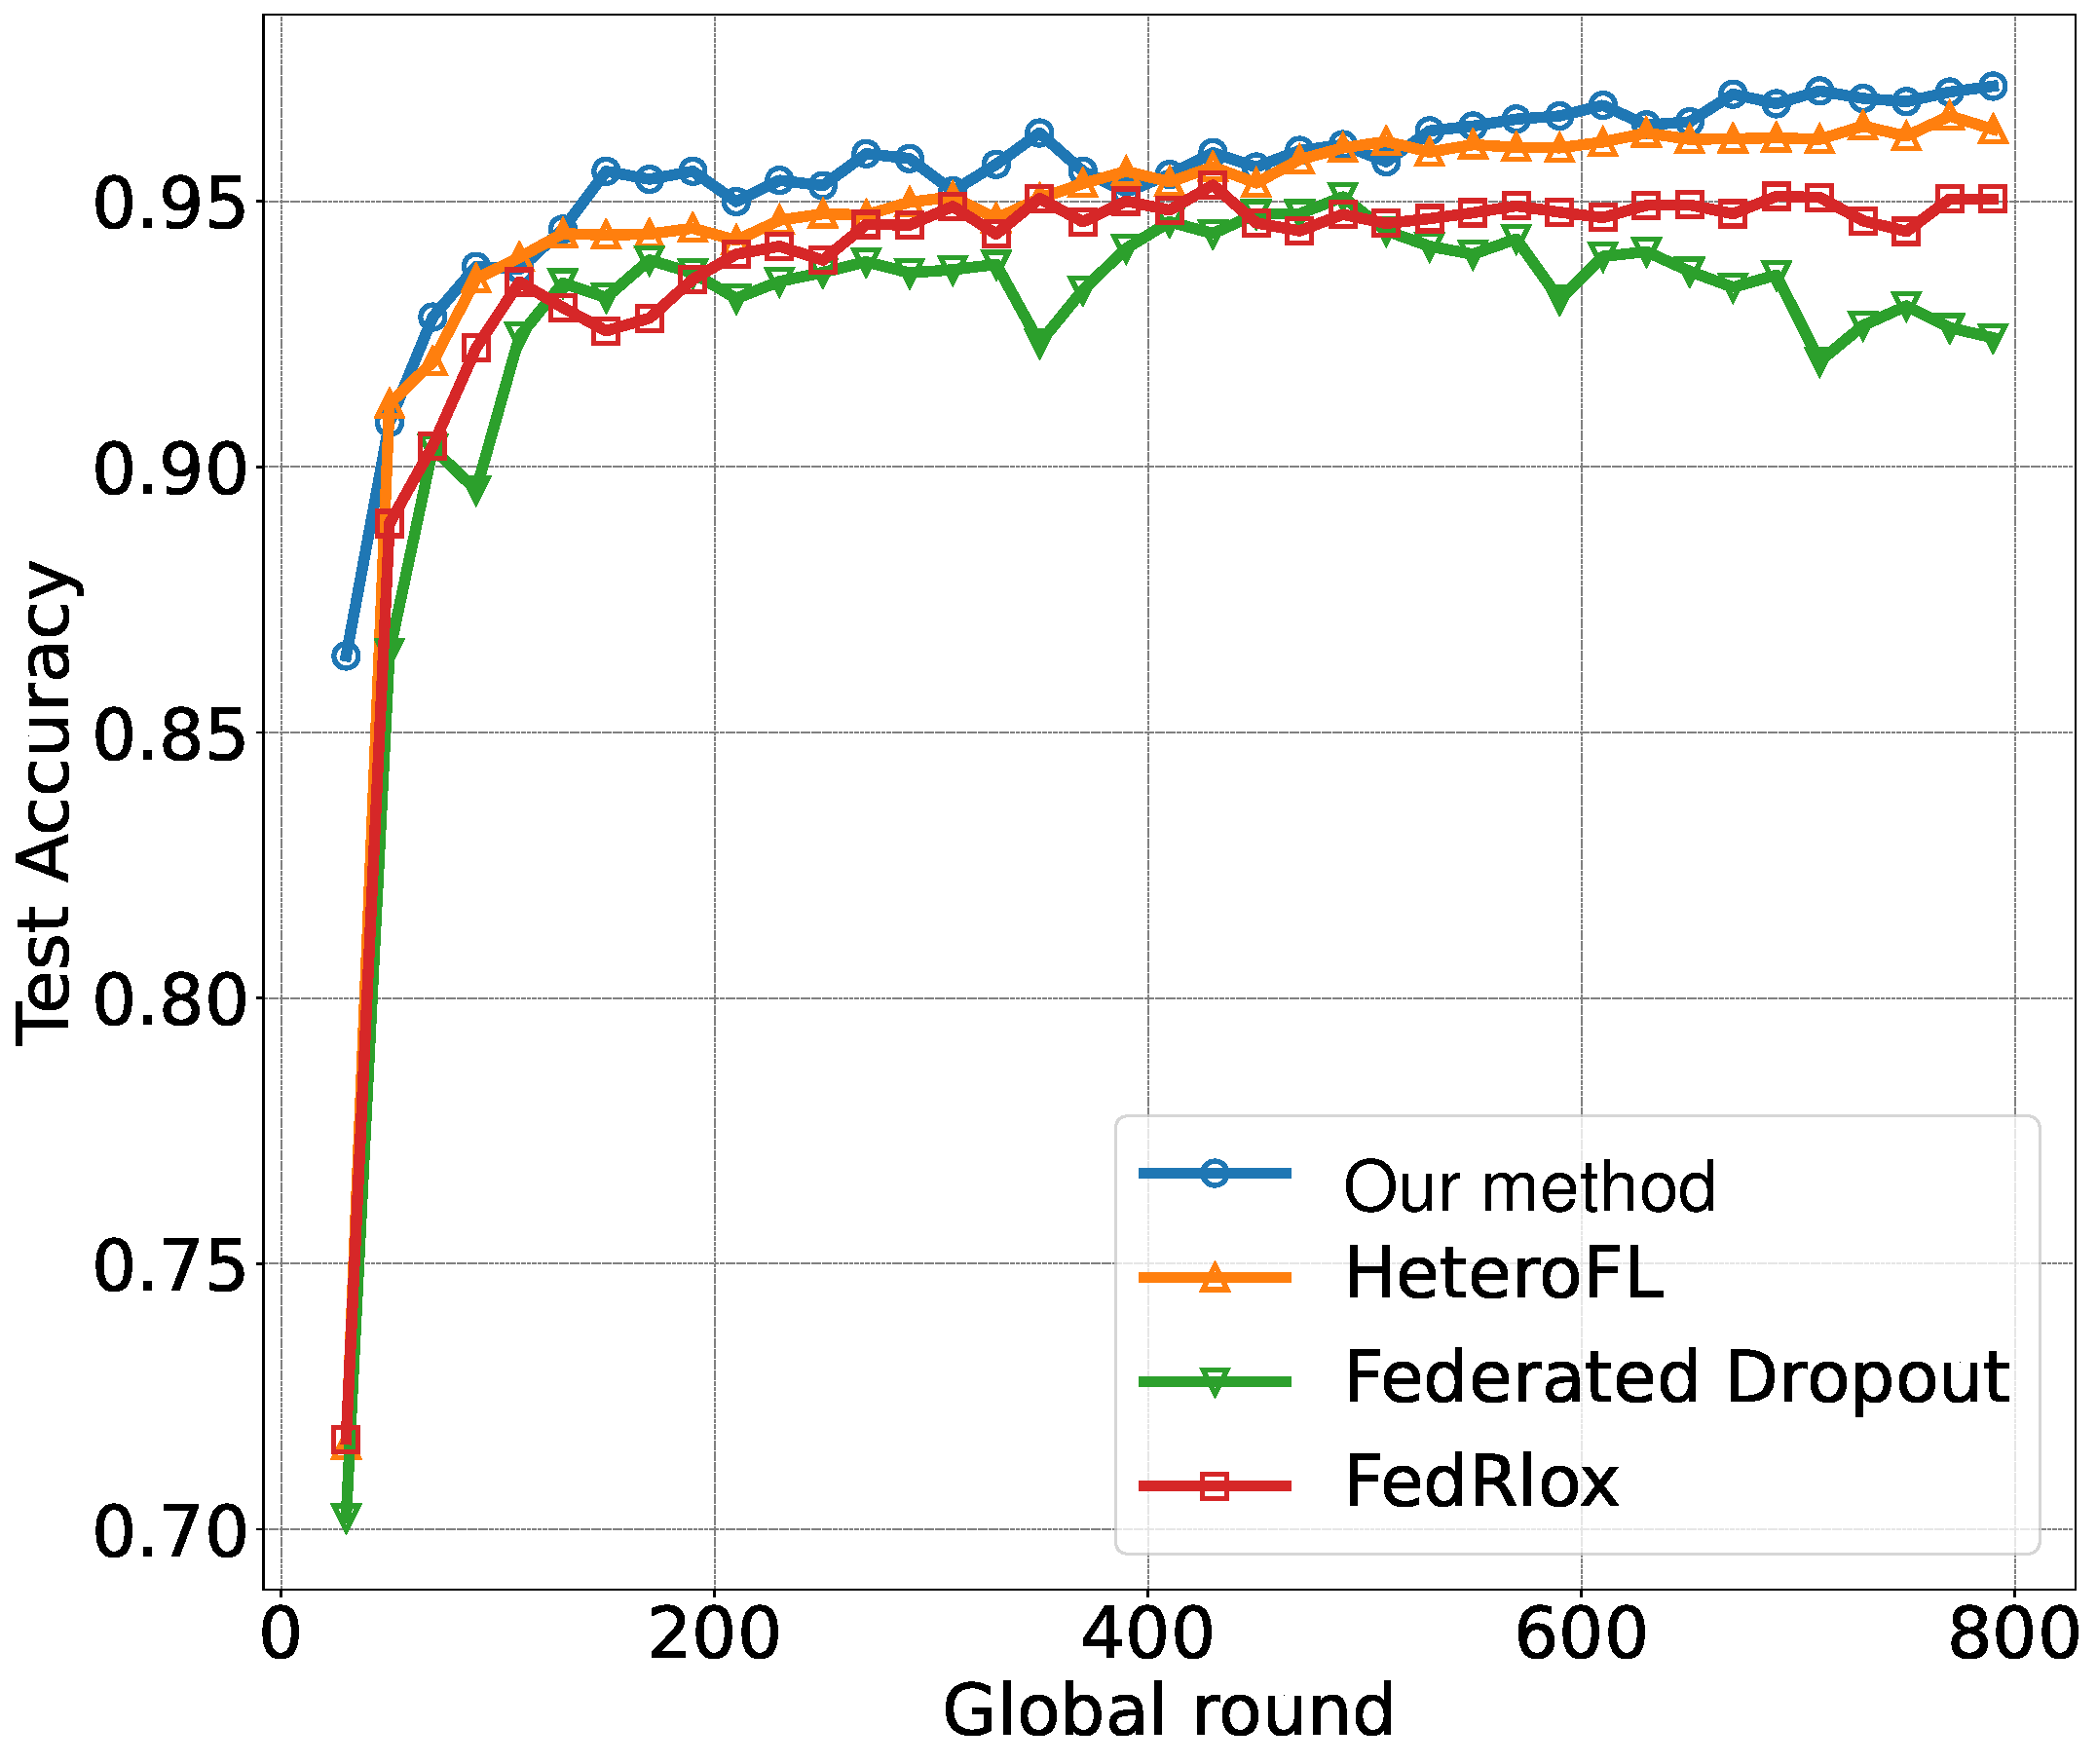
\includegraphics[width=0.92\textwidth]{picture/emnist-high-2.pdf}
    \end{minipage}
    }
    \hfill
    \subfloat[$\rho=0.4$]{
    \begin{minipage}{0.42\textwidth}
    \label{fig:emnist-high-0.4}
    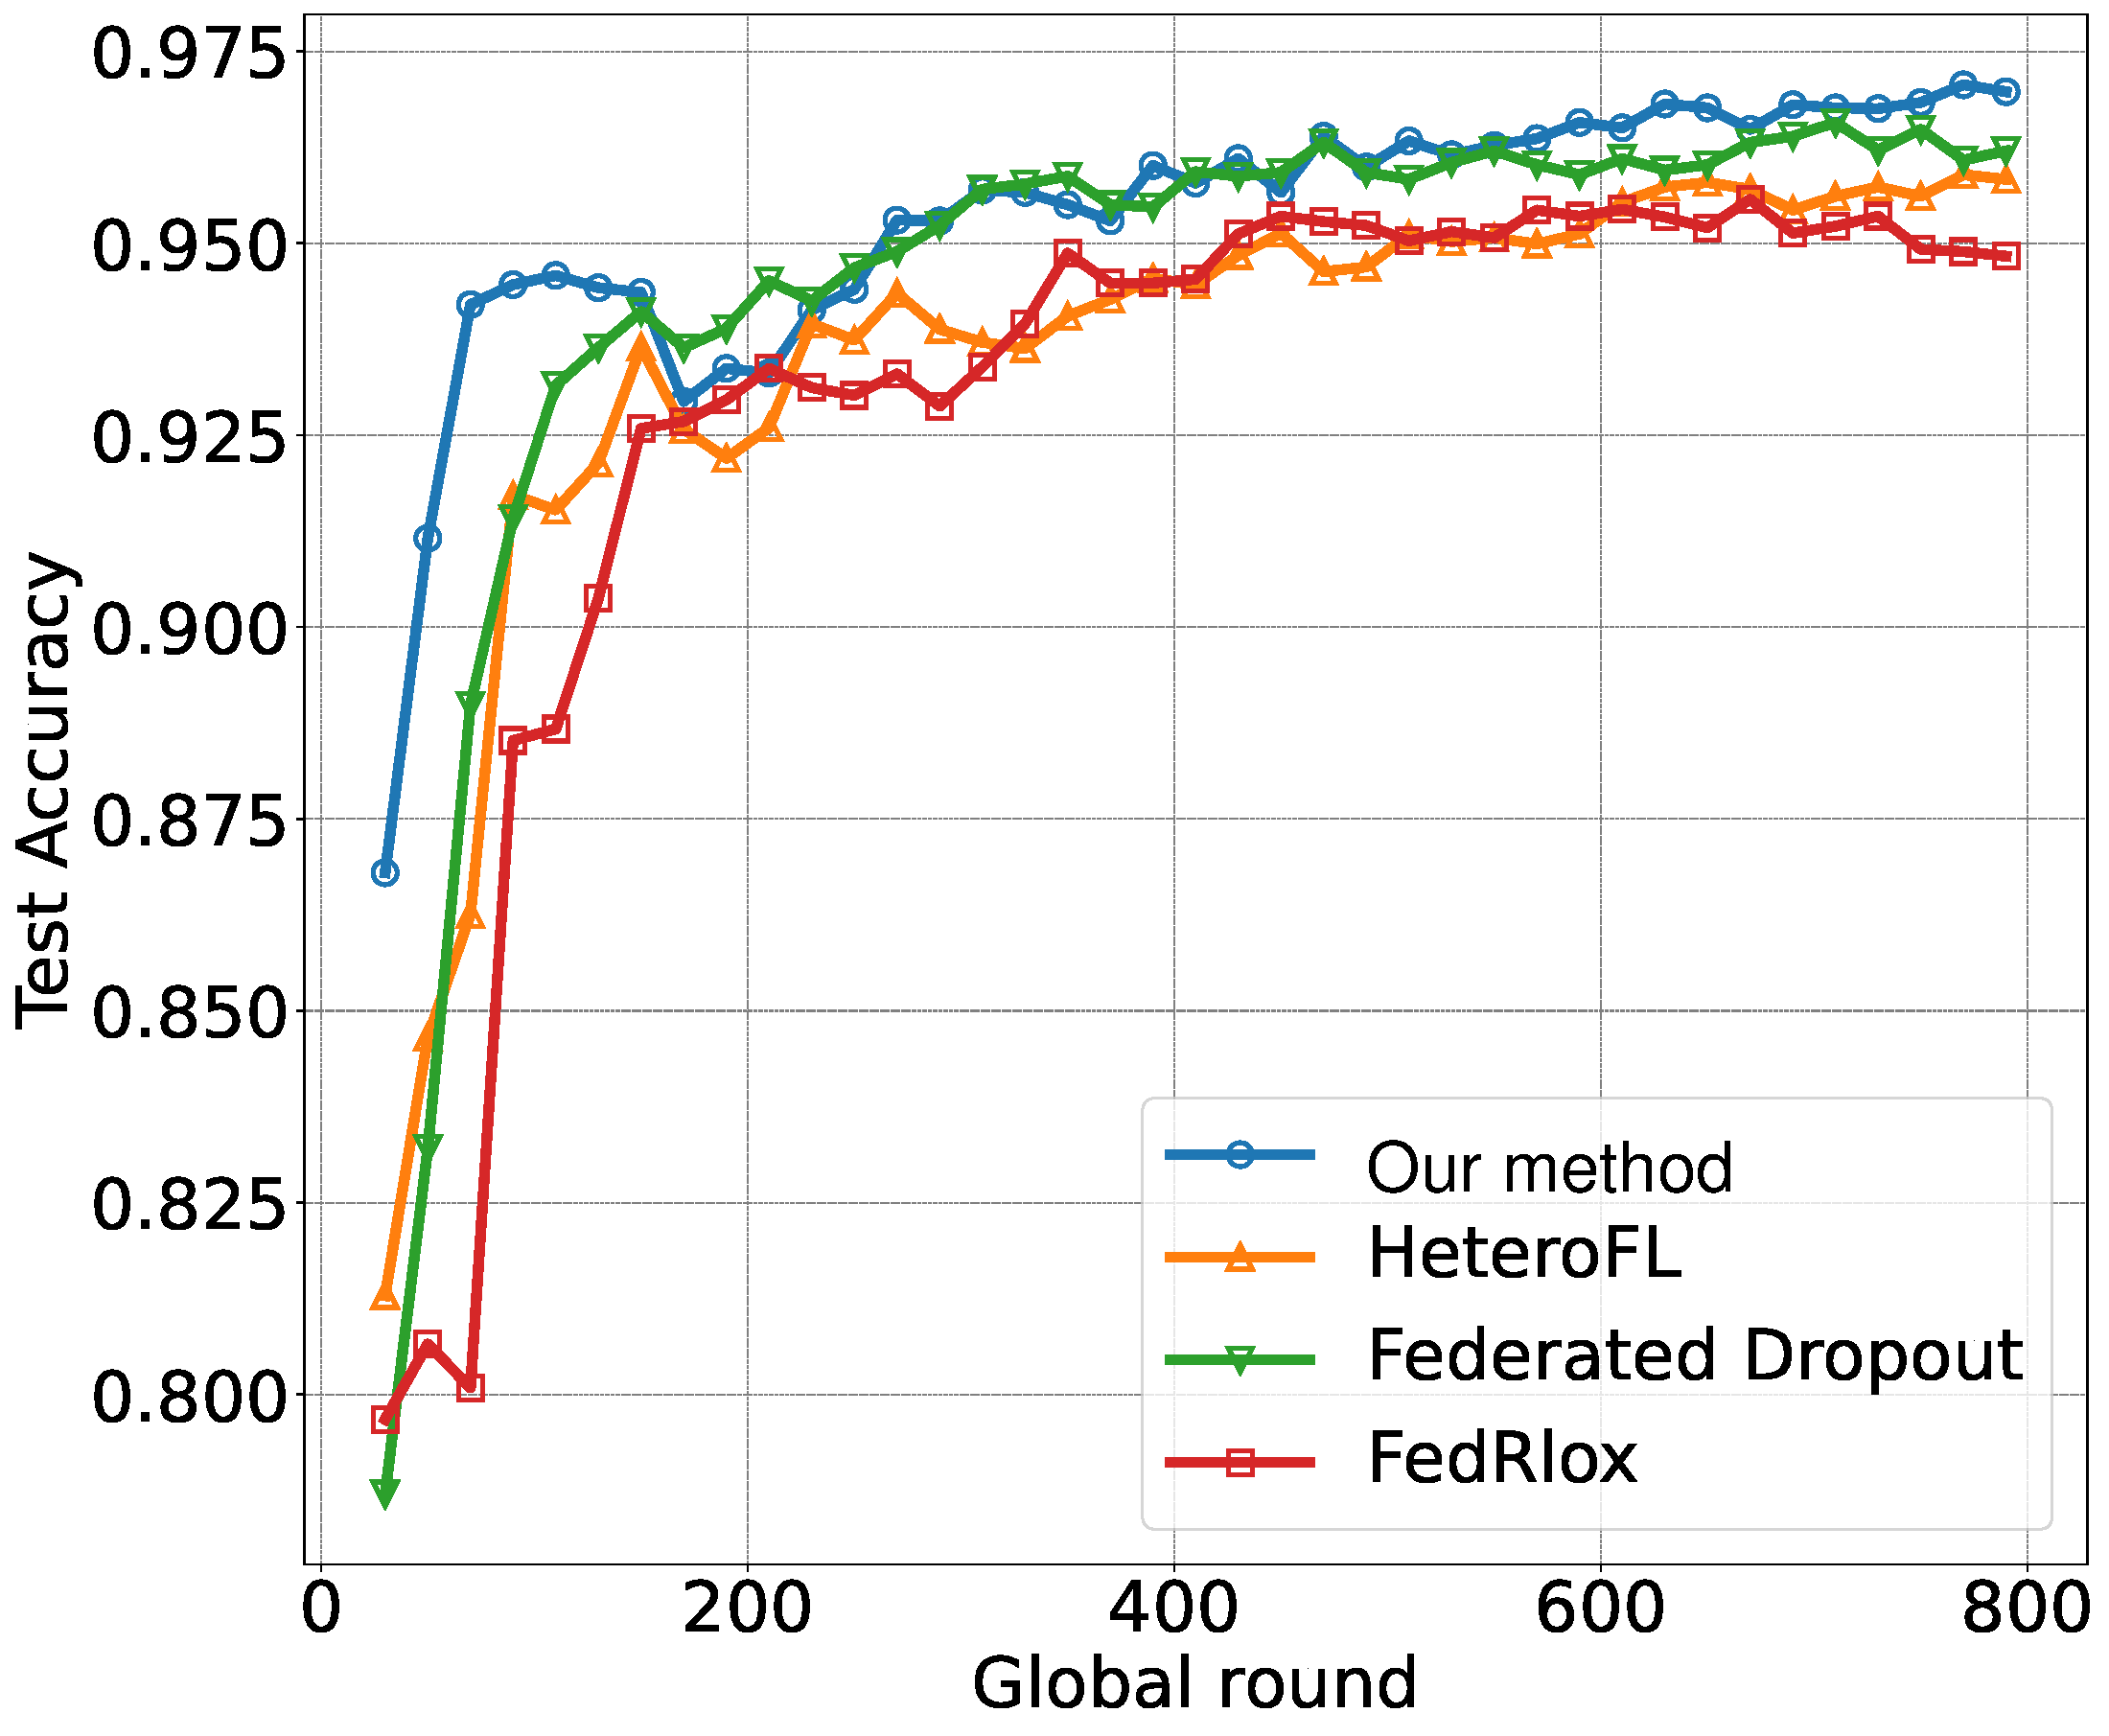
\includegraphics[width=0.92\textwidth]{picture/emnist-high-4.pdf}
    \end{minipage}
    }
    \hfill
    \subfloat[$\rho=0.6$]{
    \begin{minipage}{0.42\textwidth}
    \label{fig:emnist-high-0.6}
    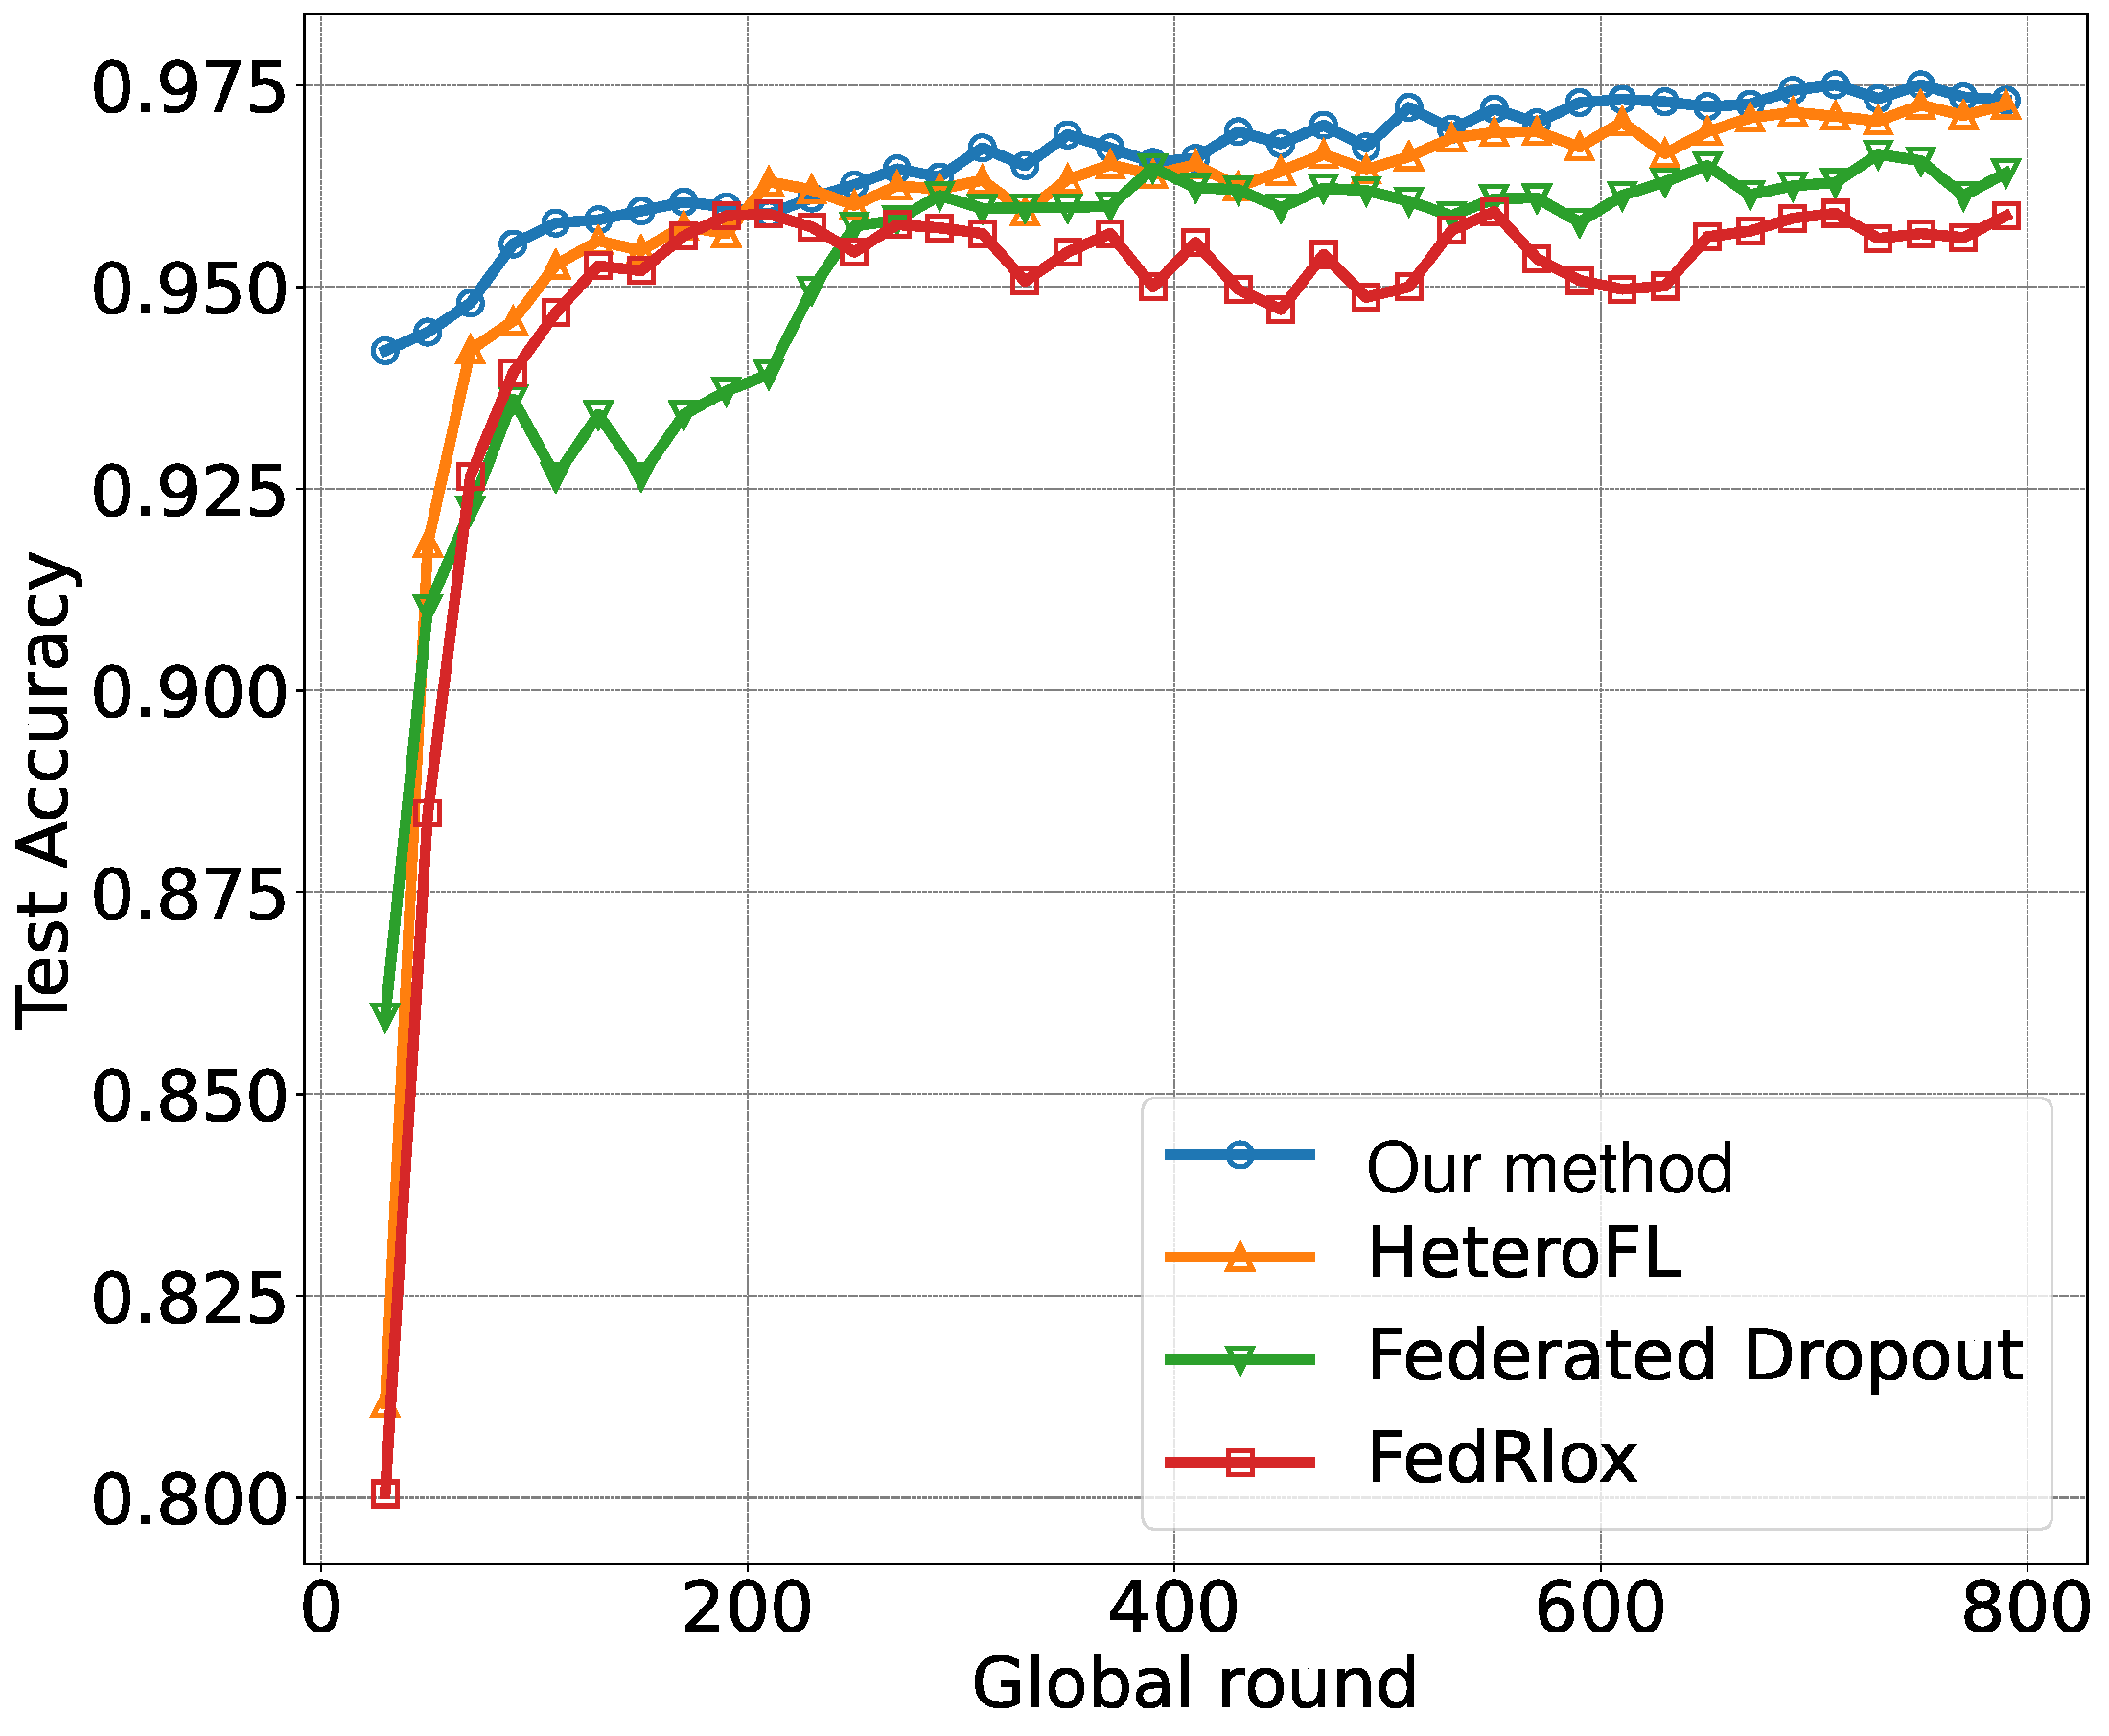
\includegraphics[width=0.92\textwidth]{picture/emnist-high-6.pdf}
    \end{minipage}
    }
    \hfill
    \subfloat[$\rho=0.8$]{
    \begin{minipage}{0.42\textwidth}
    \label{fig:emnist-high-0.8}
    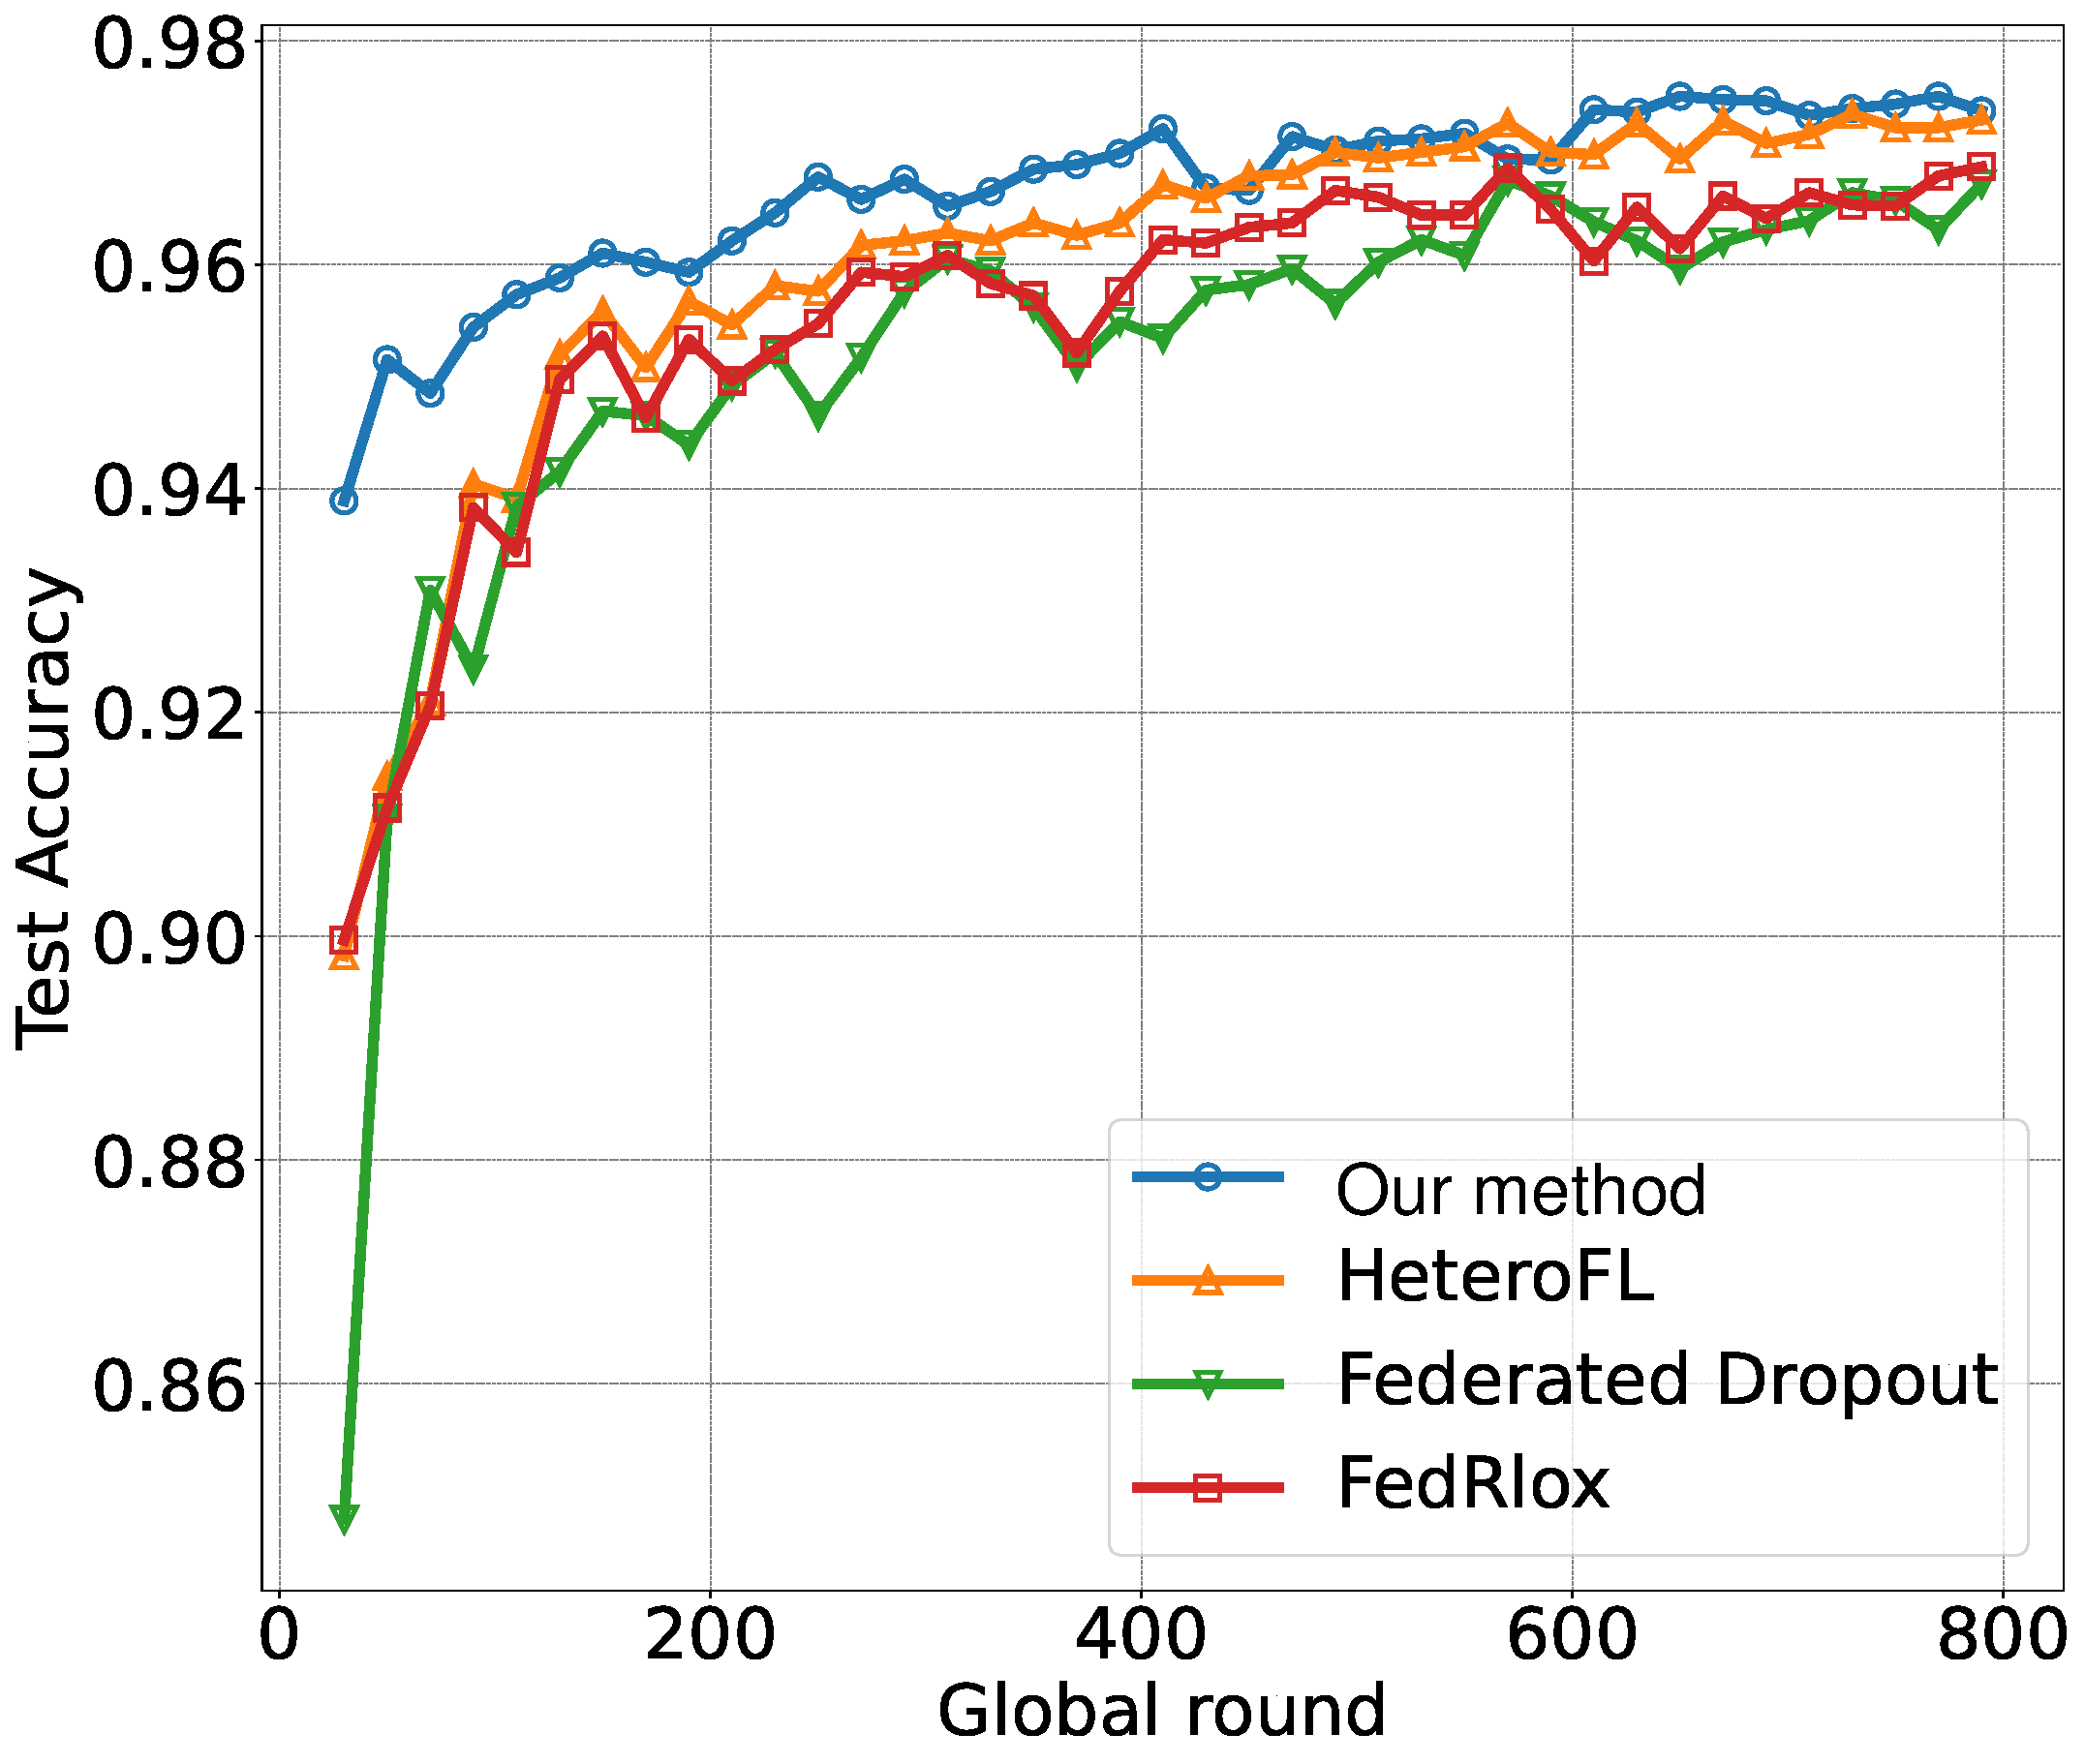
\includegraphics[width=0.92\textwidth]{picture/emnist-high-8.pdf}
    \end{minipage}
    }
    \hfill
    \begin{minipage}{0.42\textwidth}
        \subfloat[$\rho = 0.2$]{%  
            \label{fig:emnist-low-0.2}  
            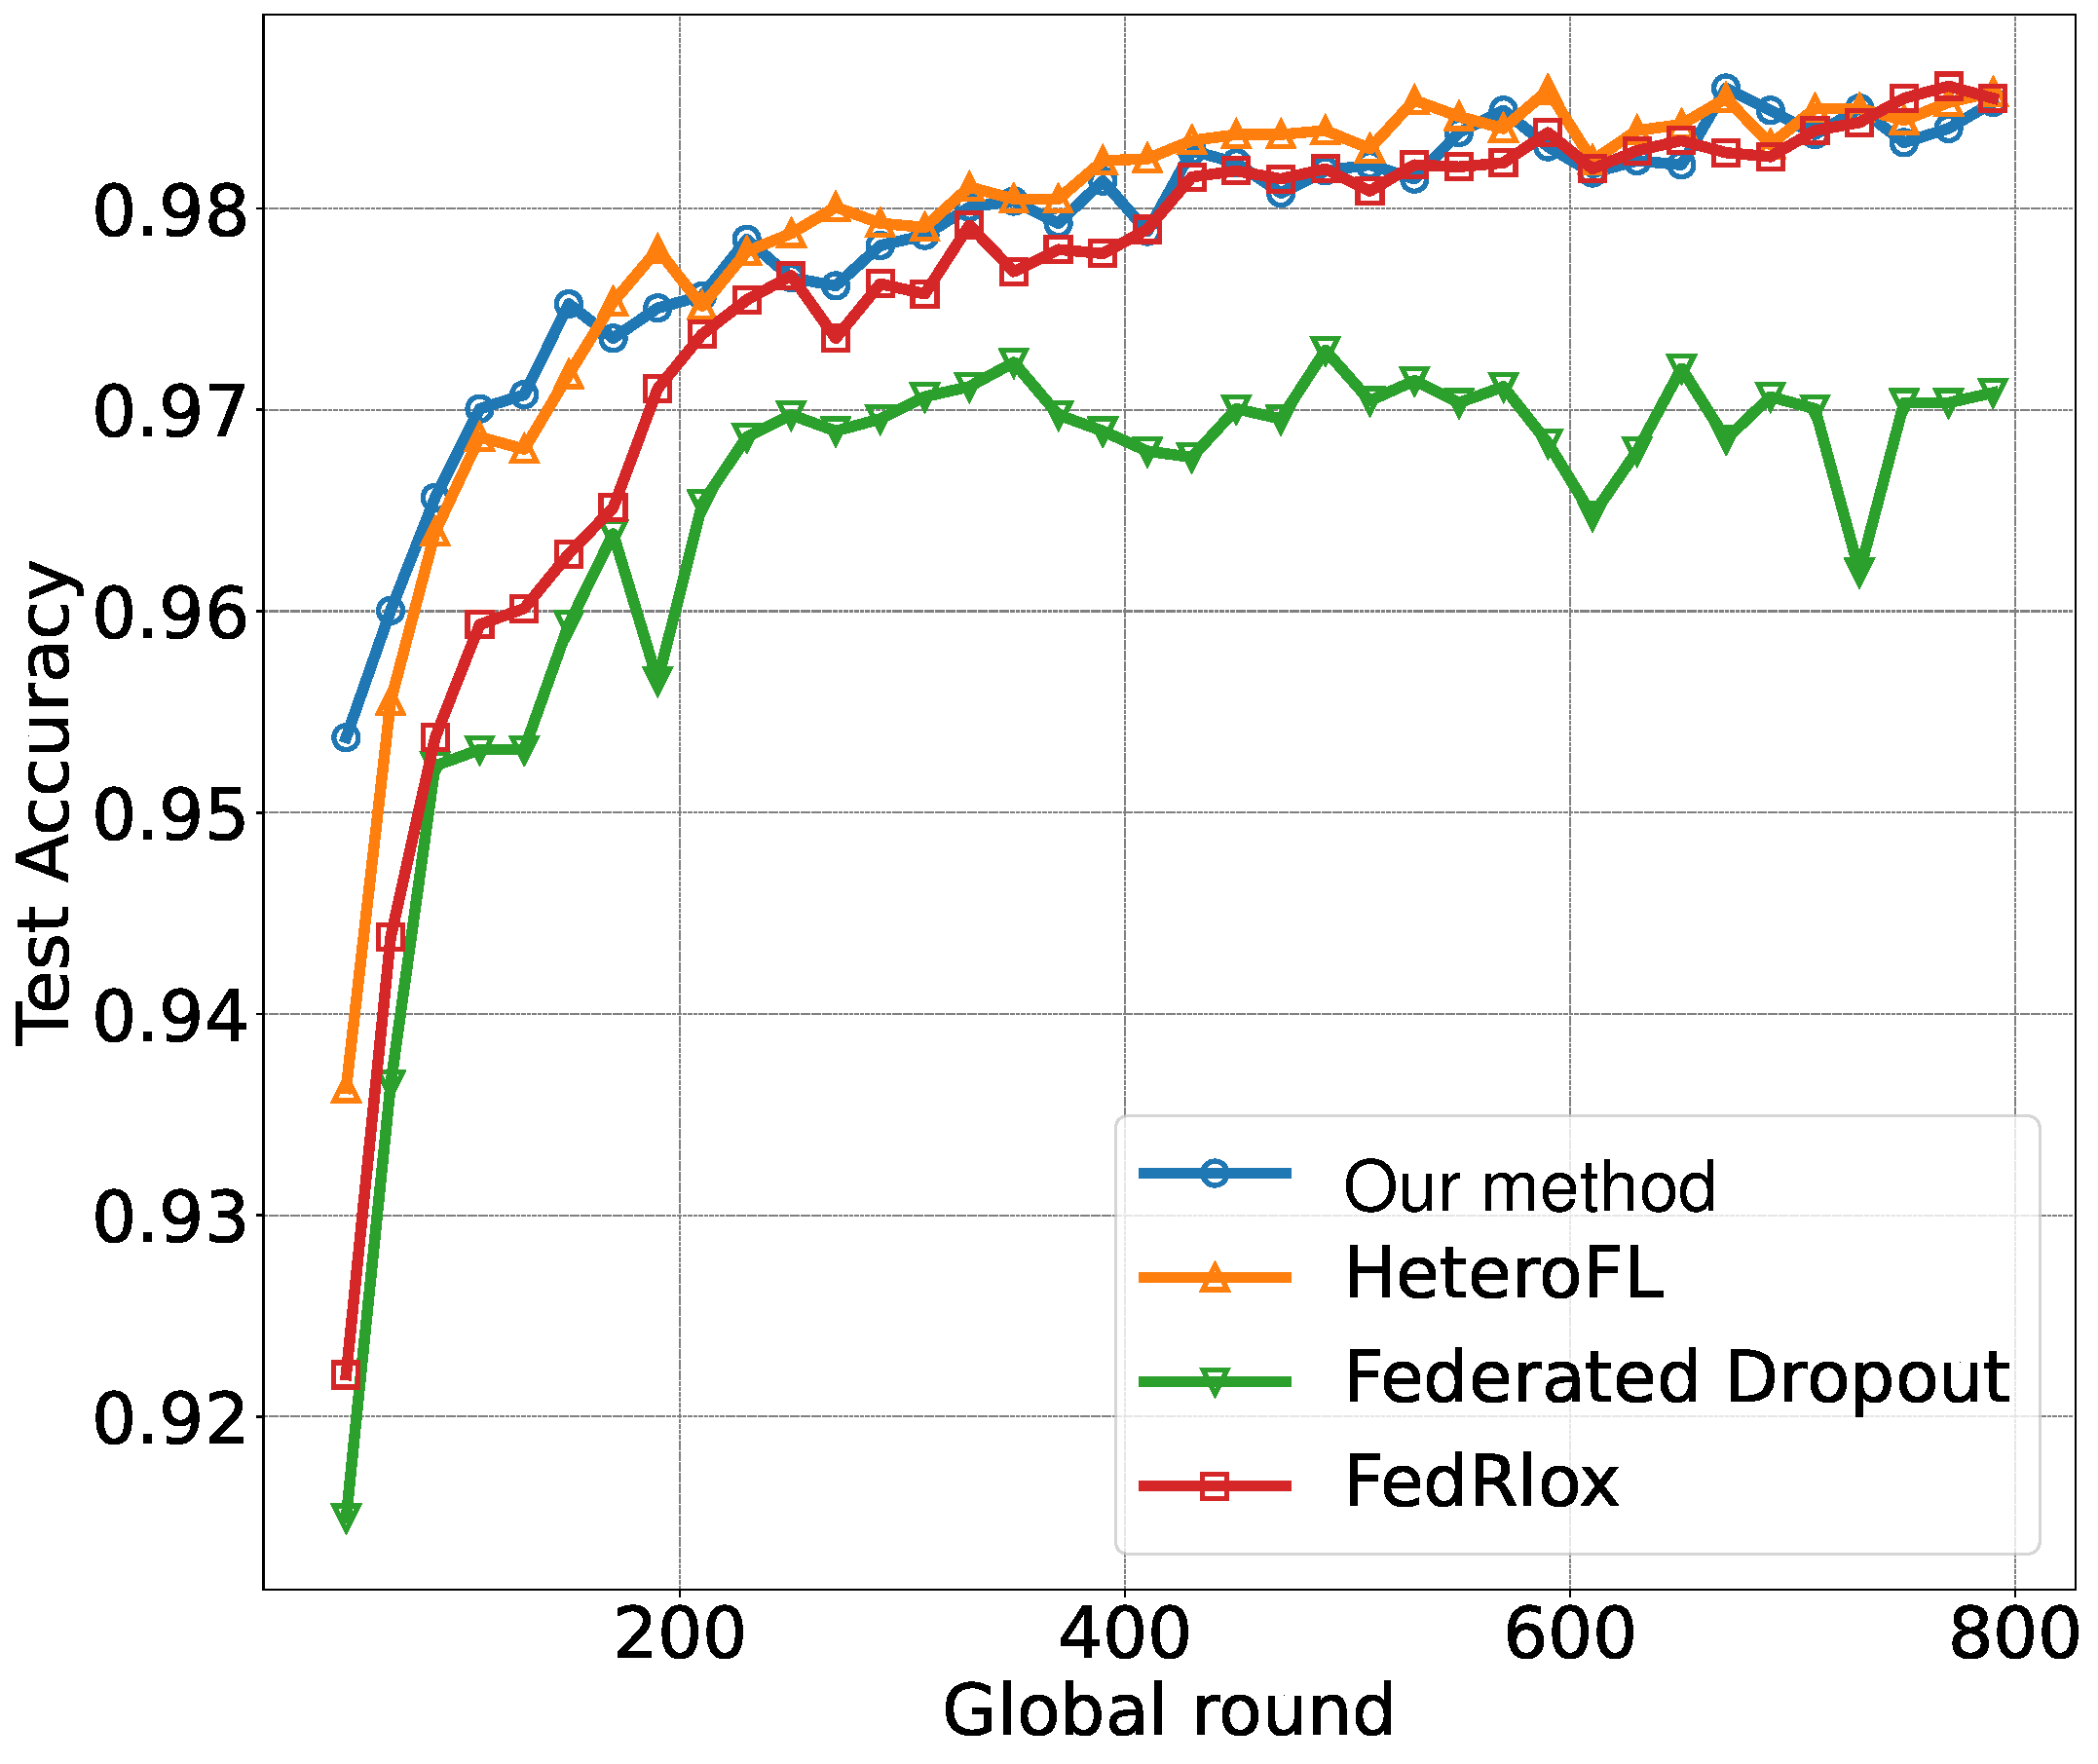
\includegraphics[width=0.92\linewidth]{picture/emnist-low-2.pdf} % 修改宽度以适应子图  
        }
        \end{minipage}
        \hfill % 水平填充  
        \begin{minipage}{0.42\textwidth}
        \subfloat[$\rho = 0.4$]{%  
            \label{fig:emnist-low-0.4}  
            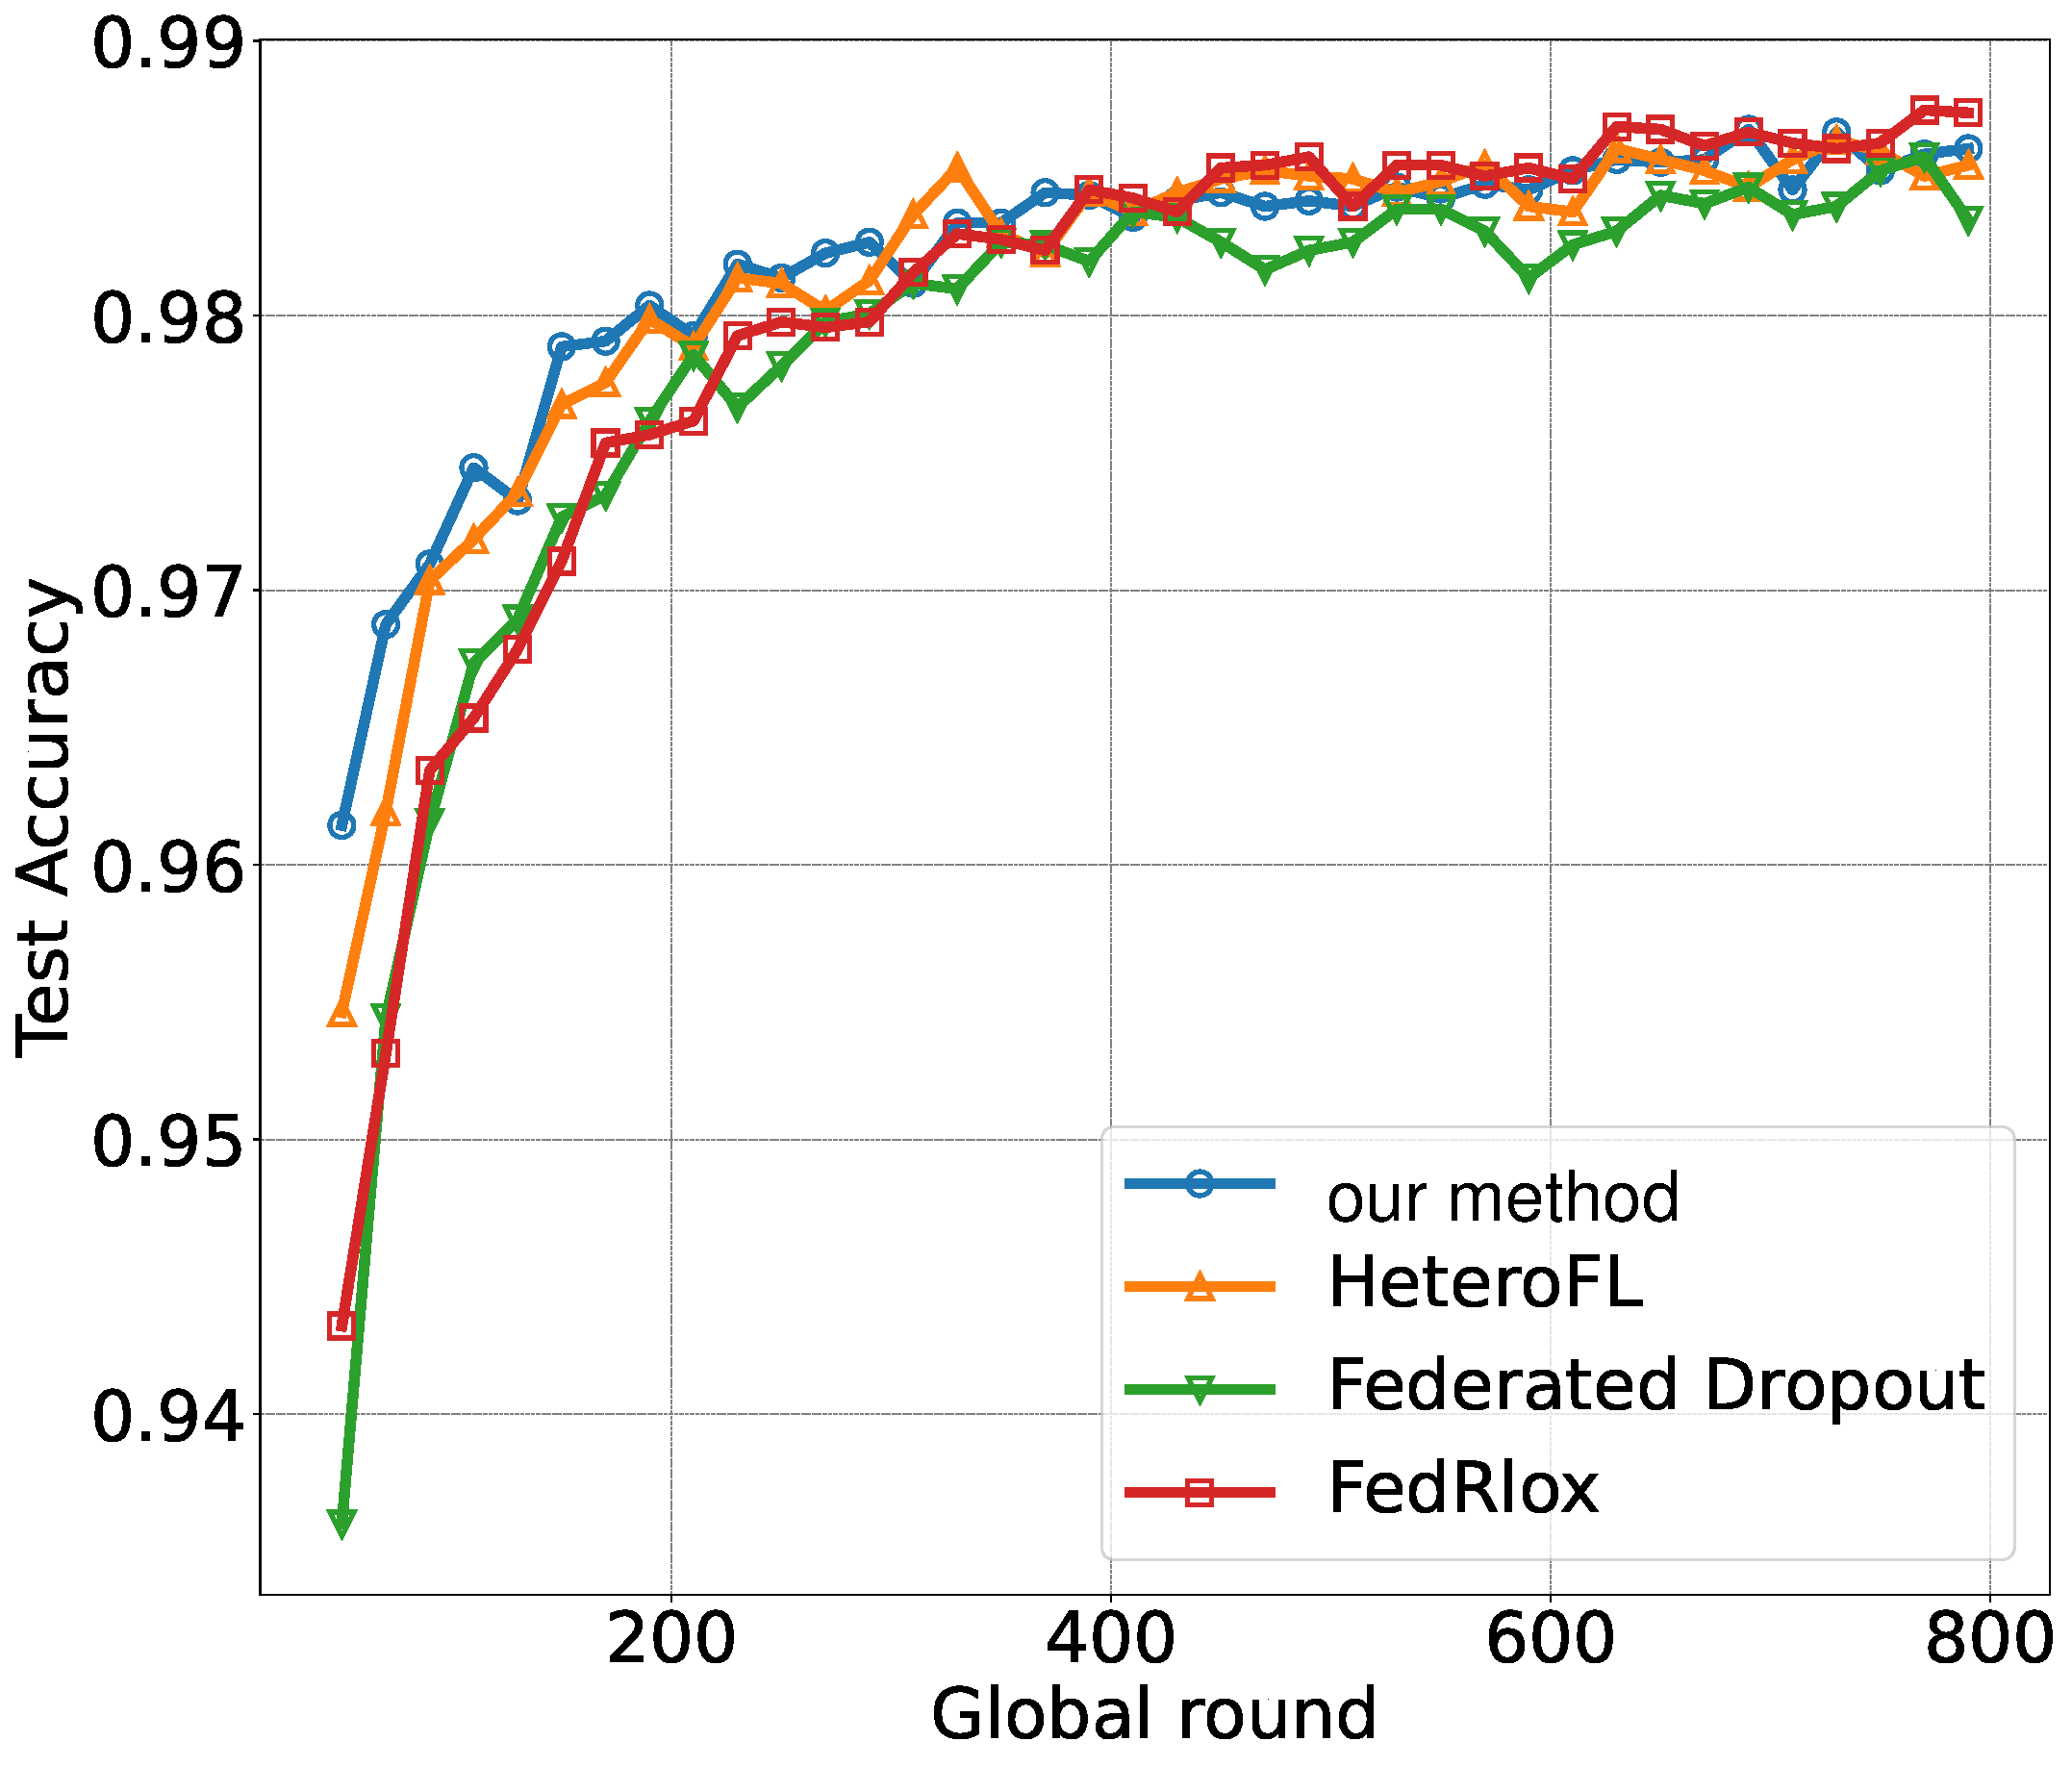
\includegraphics[width=0.92\linewidth]{picture/emnist-low-4.pdf}  
        }
        \end{minipage}
        \hfill  
        \begin{minipage}{0.42\textwidth}
        \subfloat[$\rho = 0.6$]{%  
            \label{fig:emnist-low-0.6}  
            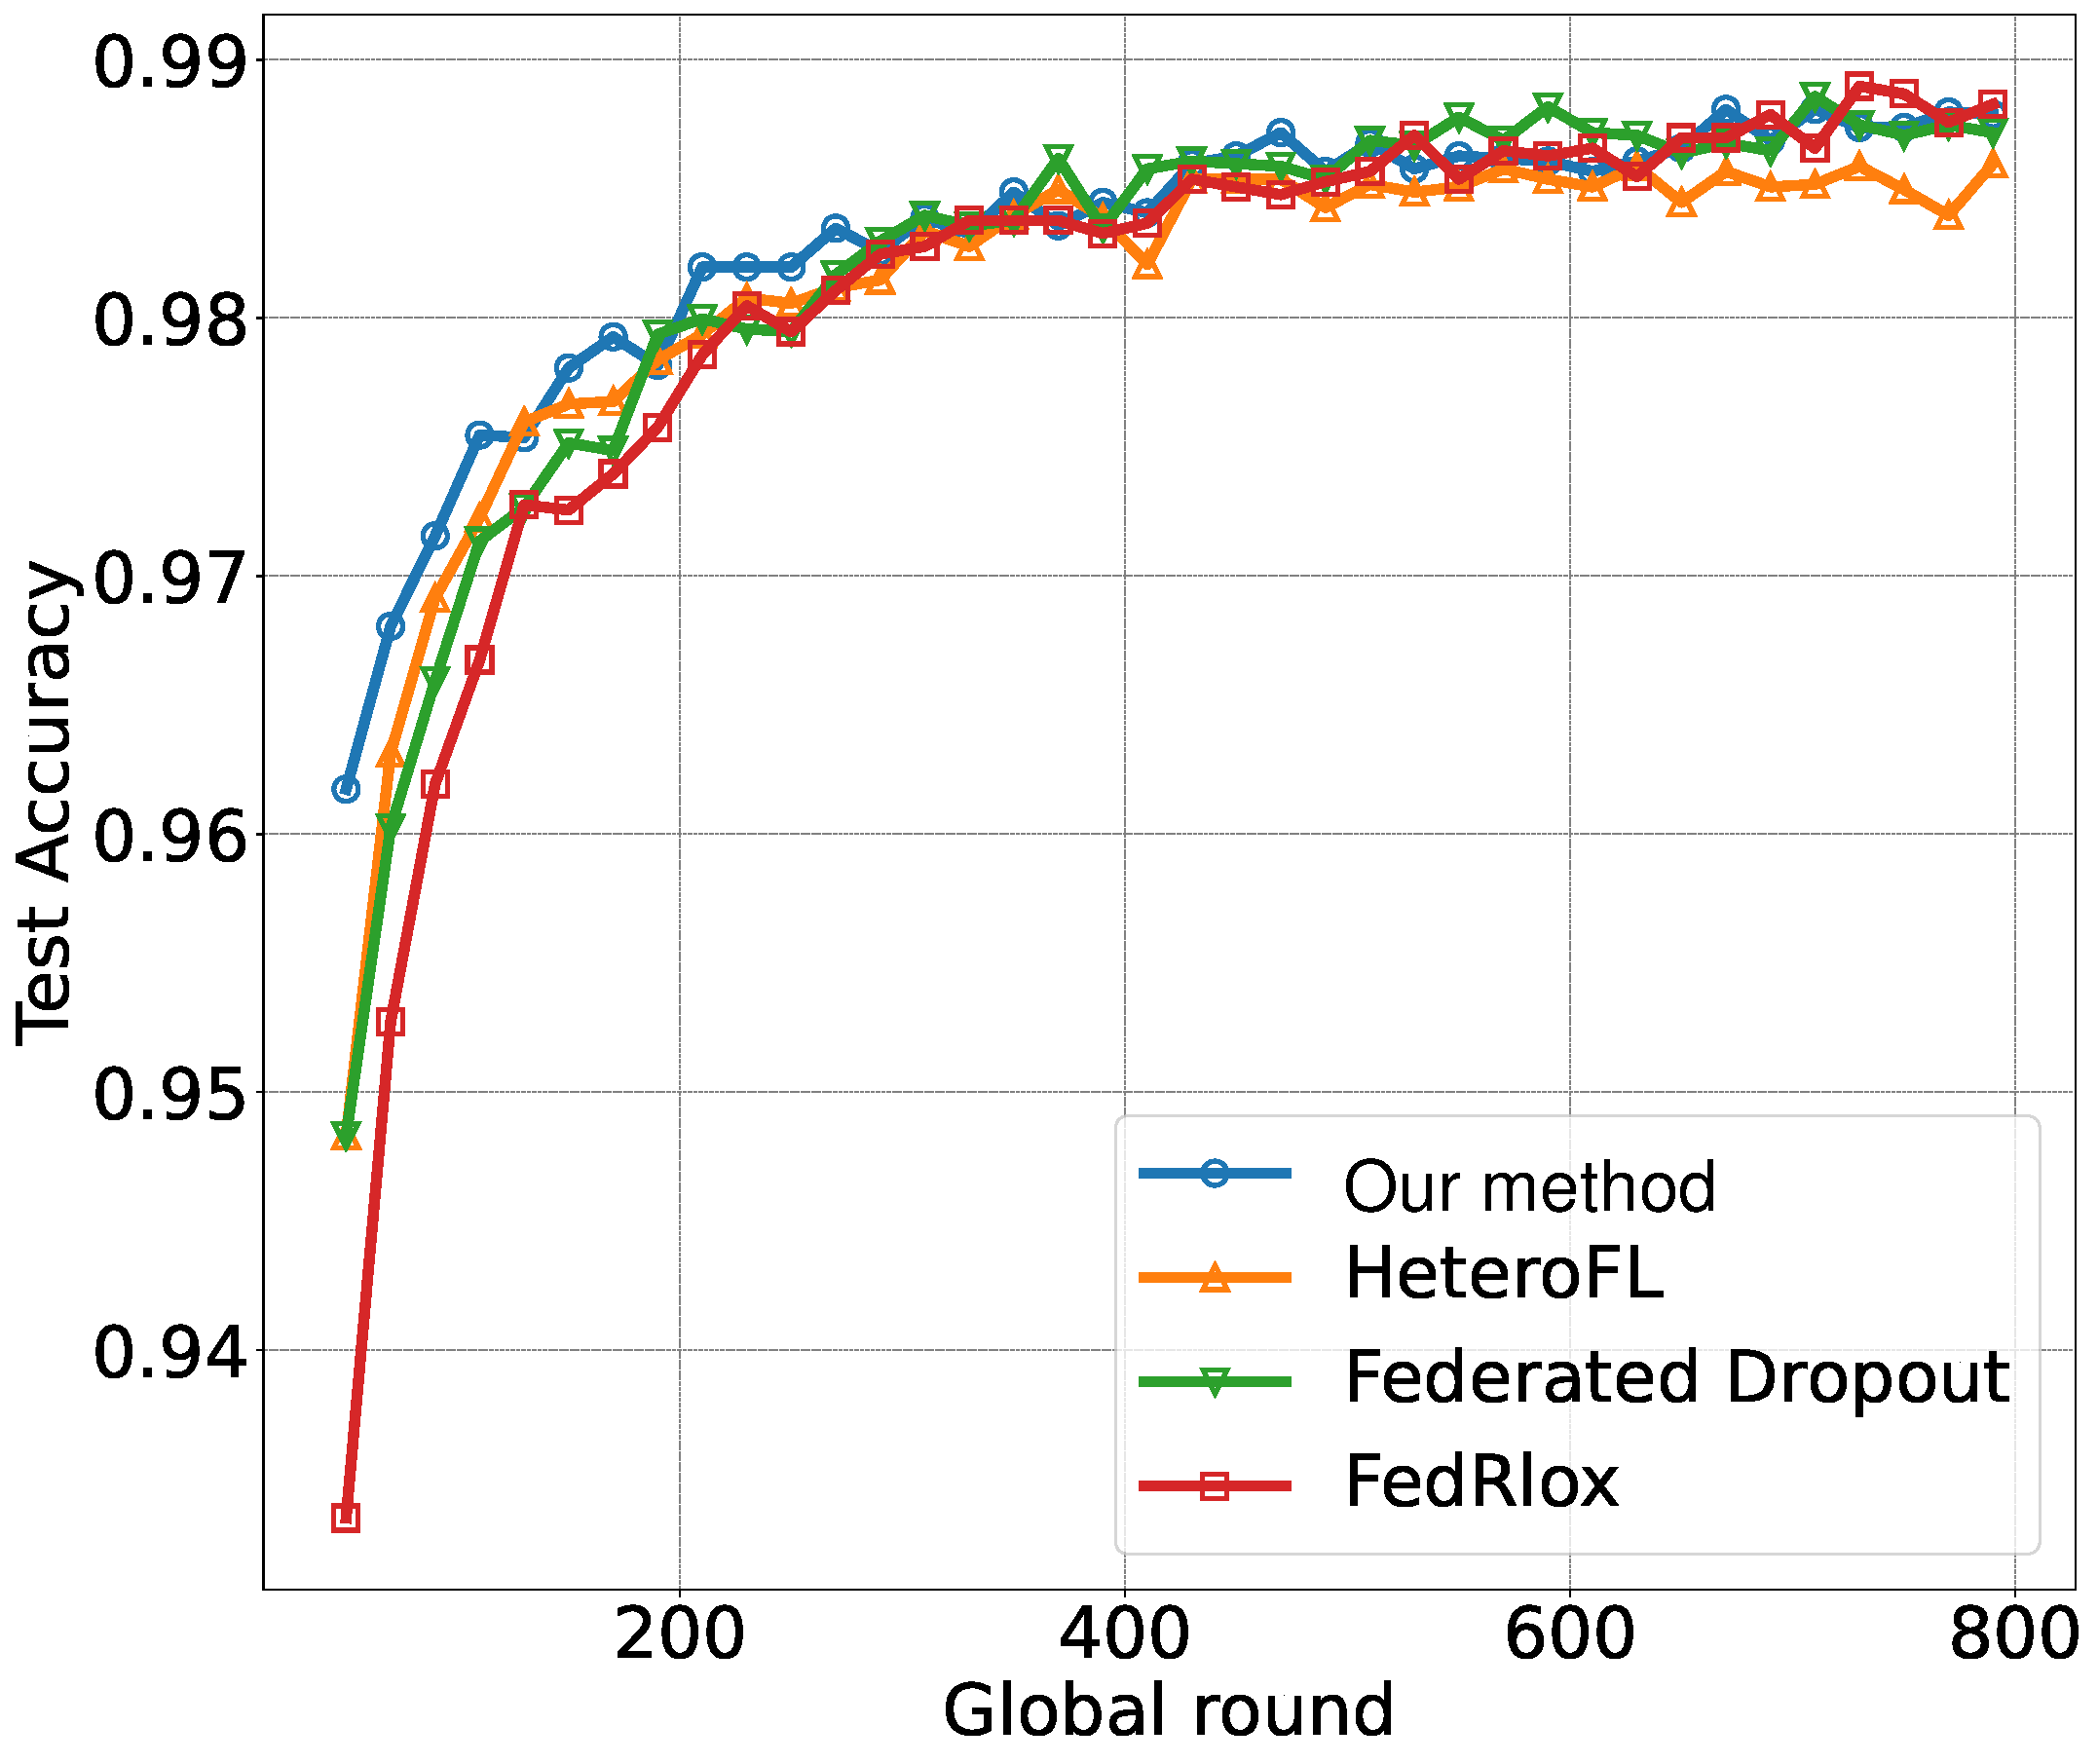
\includegraphics[width=0.92\linewidth]{picture/emnist-low-6.pdf}  
        }  
        \end{minipage}
        \hfill  
        \begin{minipage}{0.42\textwidth}
        \subfloat[$\rho = 0.8$]{%  
            \label{fig:emnist-low-0.8}  
            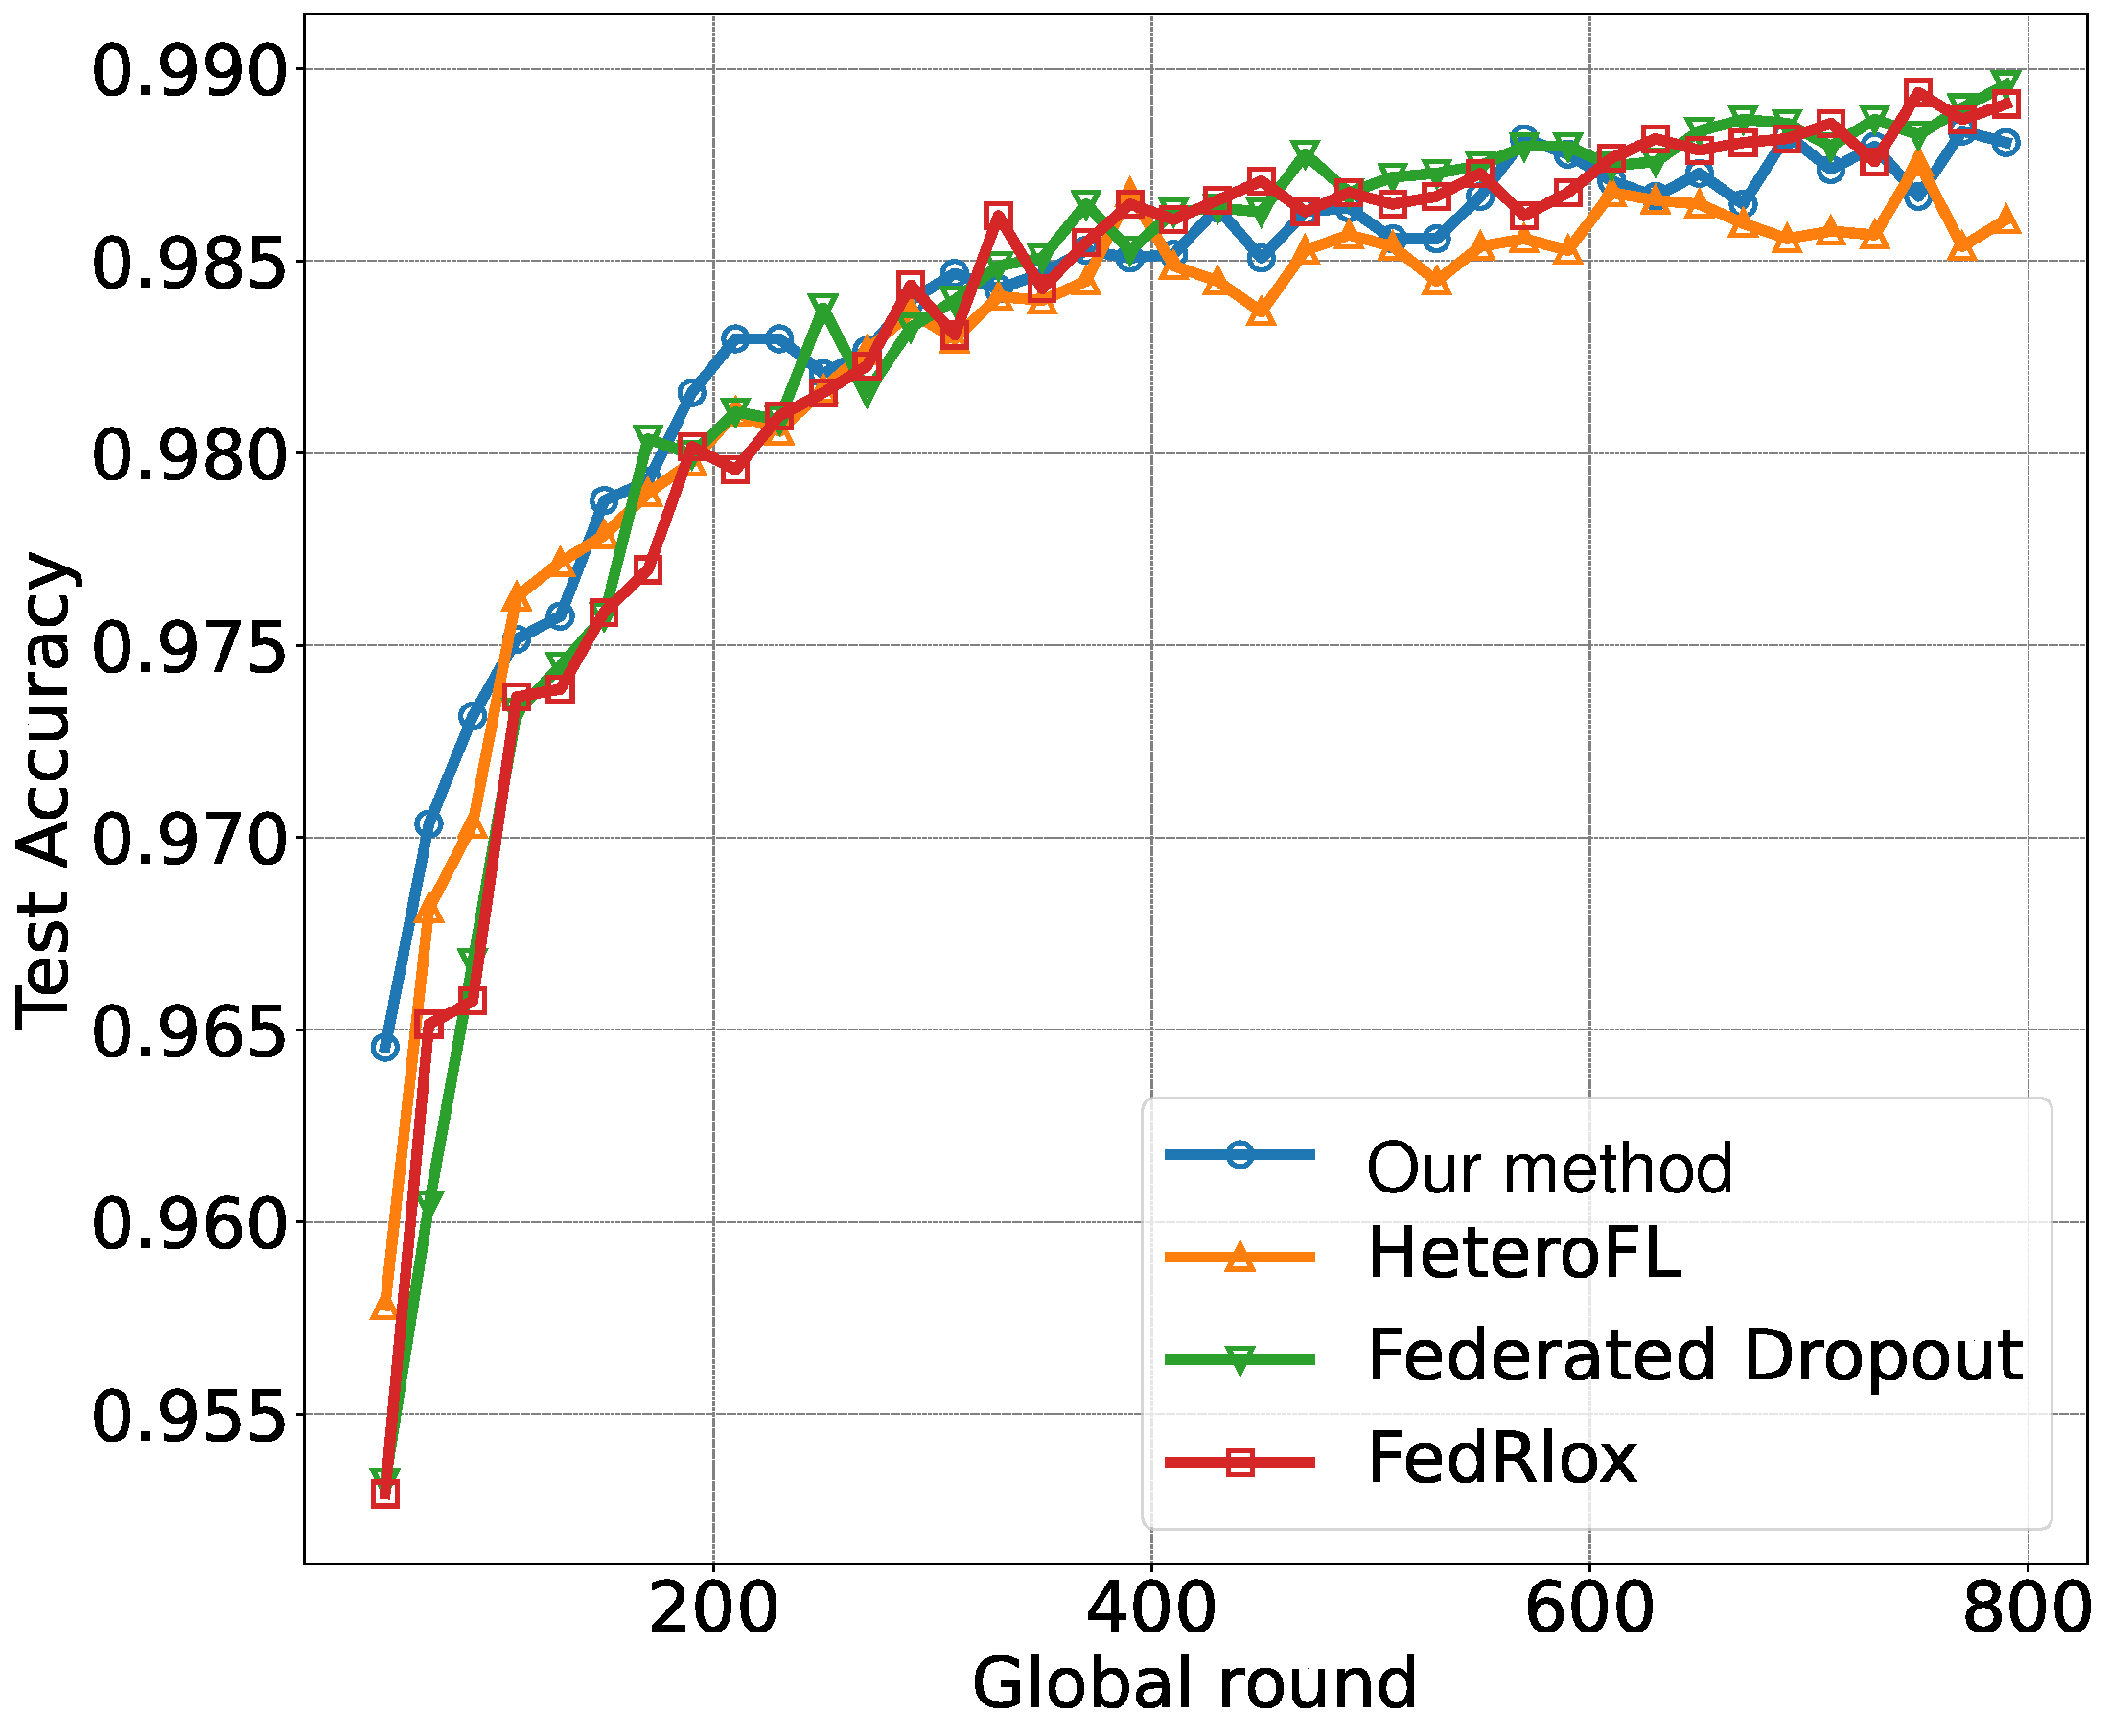
\includegraphics[width=0.92\linewidth]{picture/emnist-low-8.pdf}  
        }  
        \end{minipage}
    \caption{高低数据异质性下EMNIST数据训练细节}
    \label{fig:emnist-high-high}
    % \vspace{-0.5cm}
\end{figure}

%ppppppppppppppppppppppppppppppppppppppppppppppp
% emnist-low  
% \begin{figure}[thbp]  
%     \centering % 确保子图居中  
%     \begin{minipage}{0.45\textwidth}
%     \subfloat[$\rho = 0.2$]{%  
%         \label{fig:emnist-low-0.2}  
%         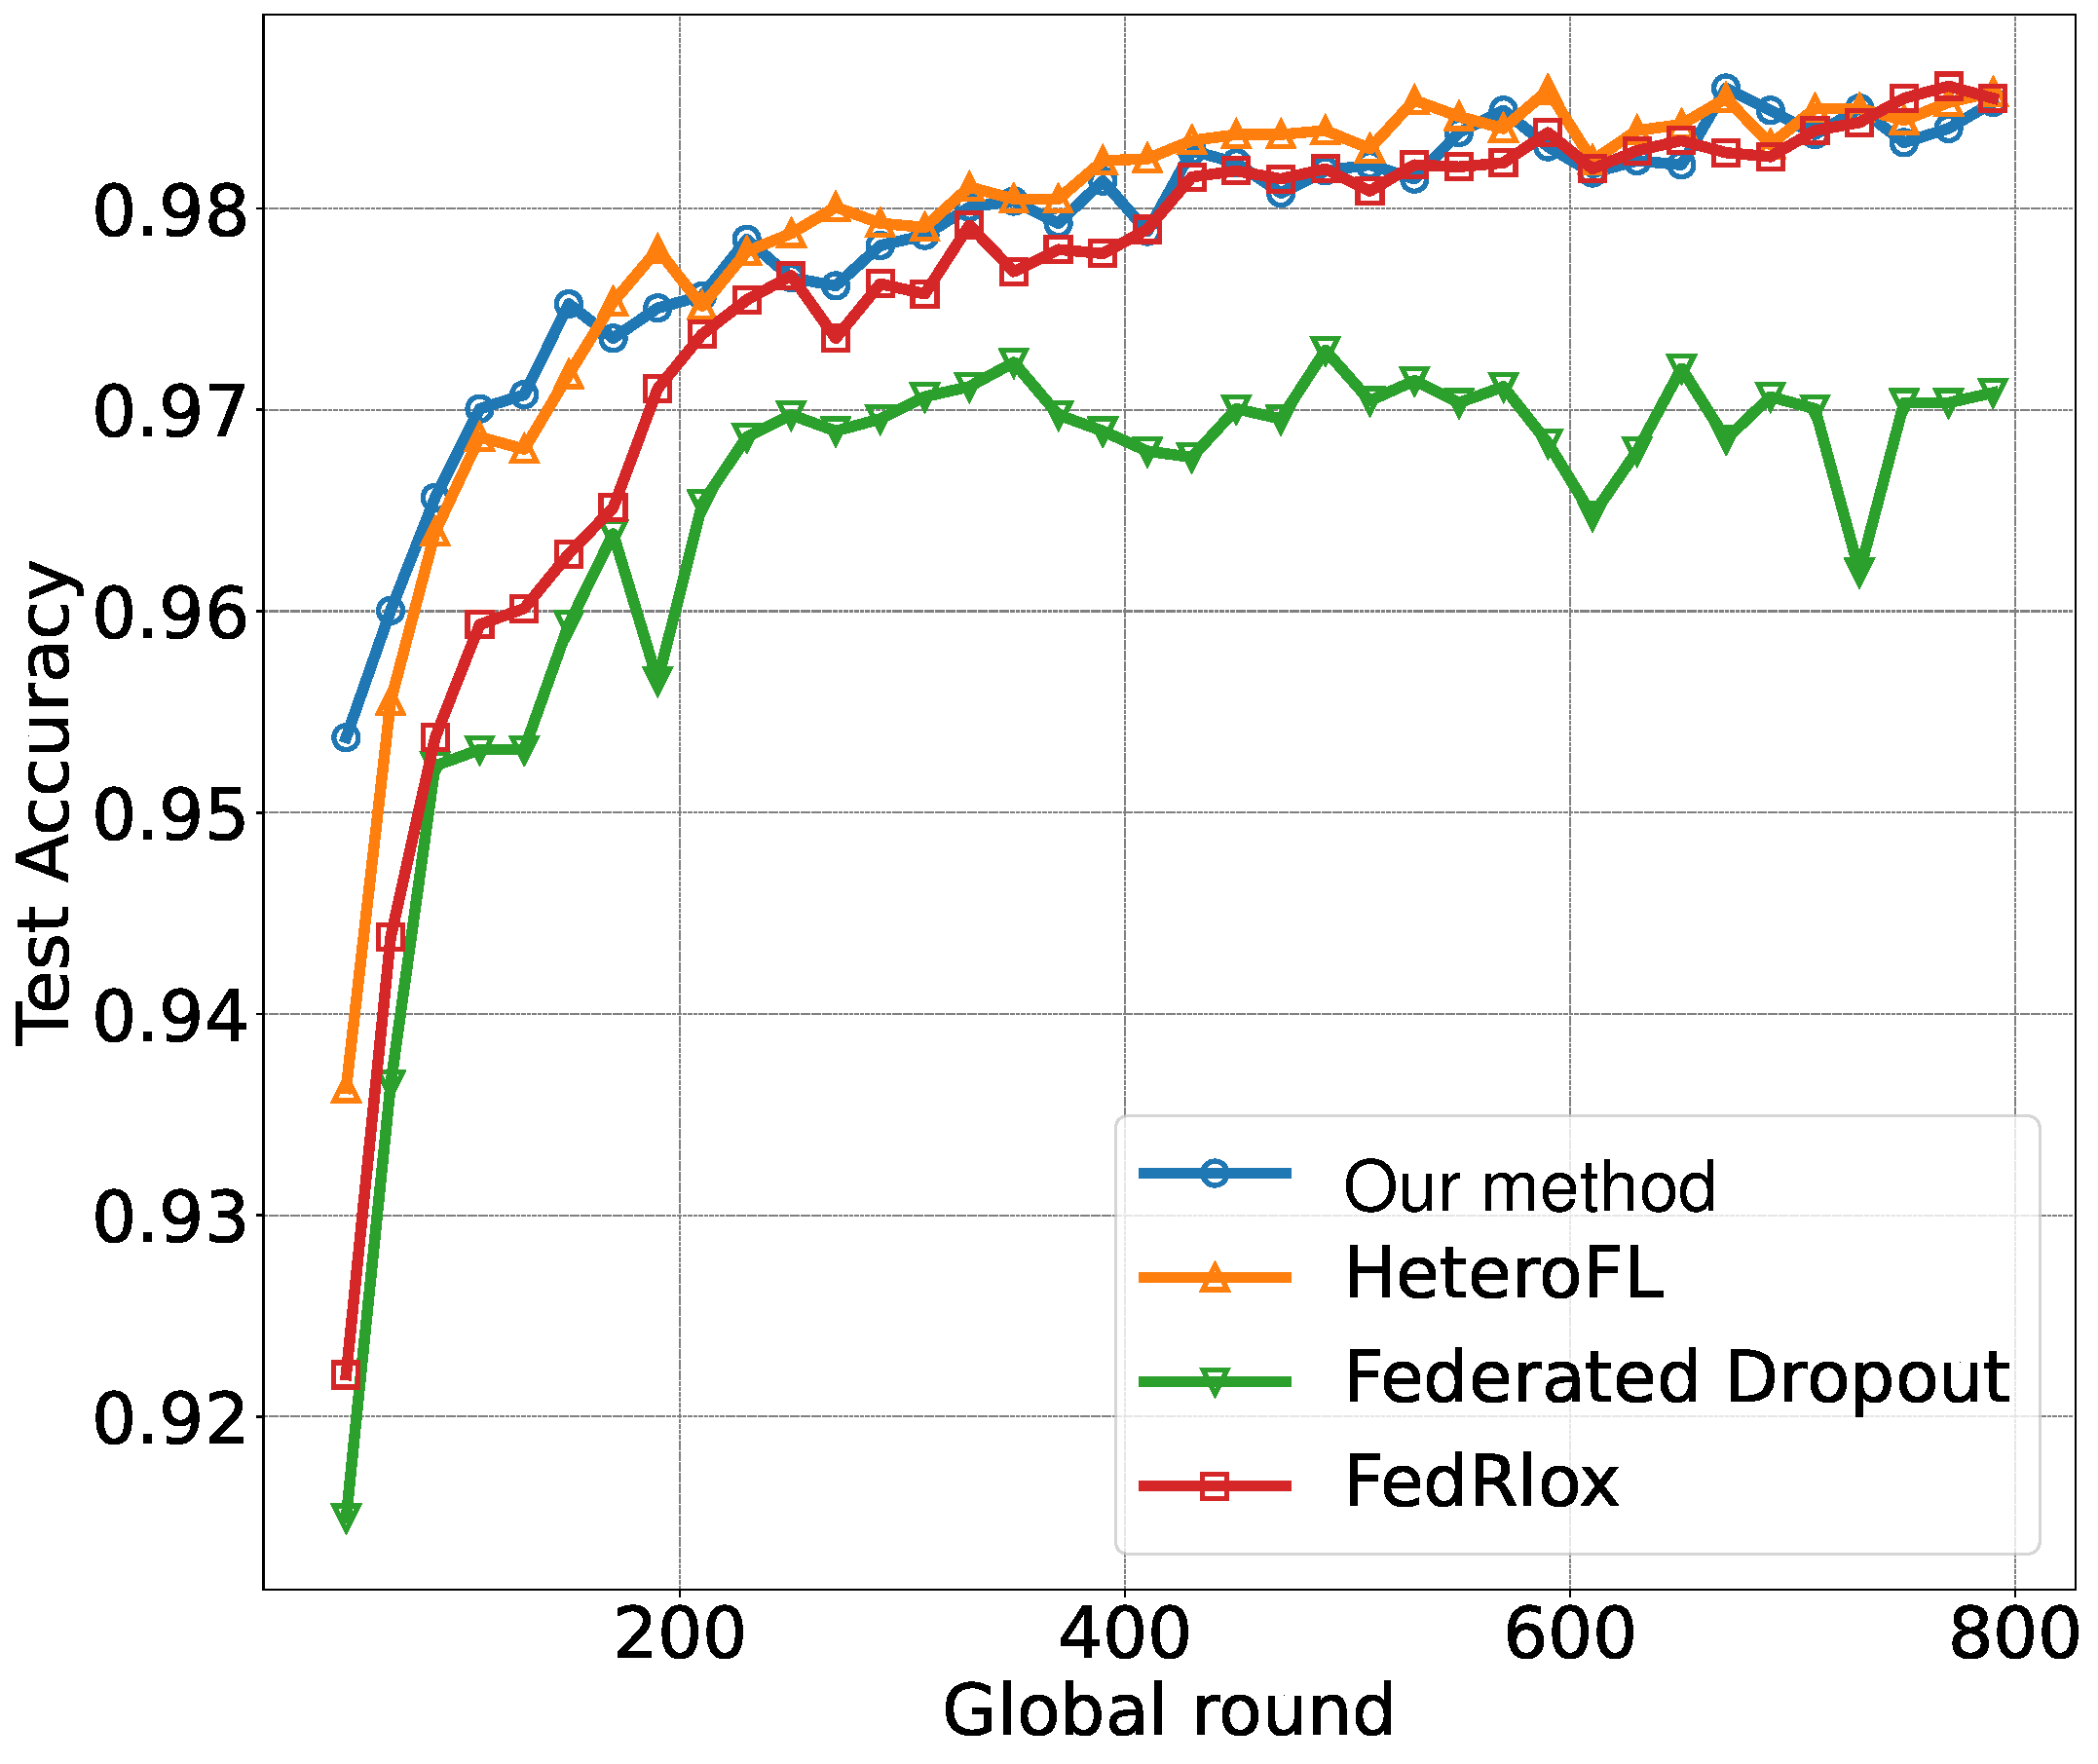
\includegraphics[width=0.9\linewidth]{picture/emnist-low-2.pdf} % 修改宽度以适应子图  
%     }
%     \end{minipage}
%     \hfill % 水平填充  
%     \begin{minipage}{0.45\textwidth}
%     \subfloat[$\rho = 0.4$]{%  
%         \label{fig:emnist-low-0.4}  
%         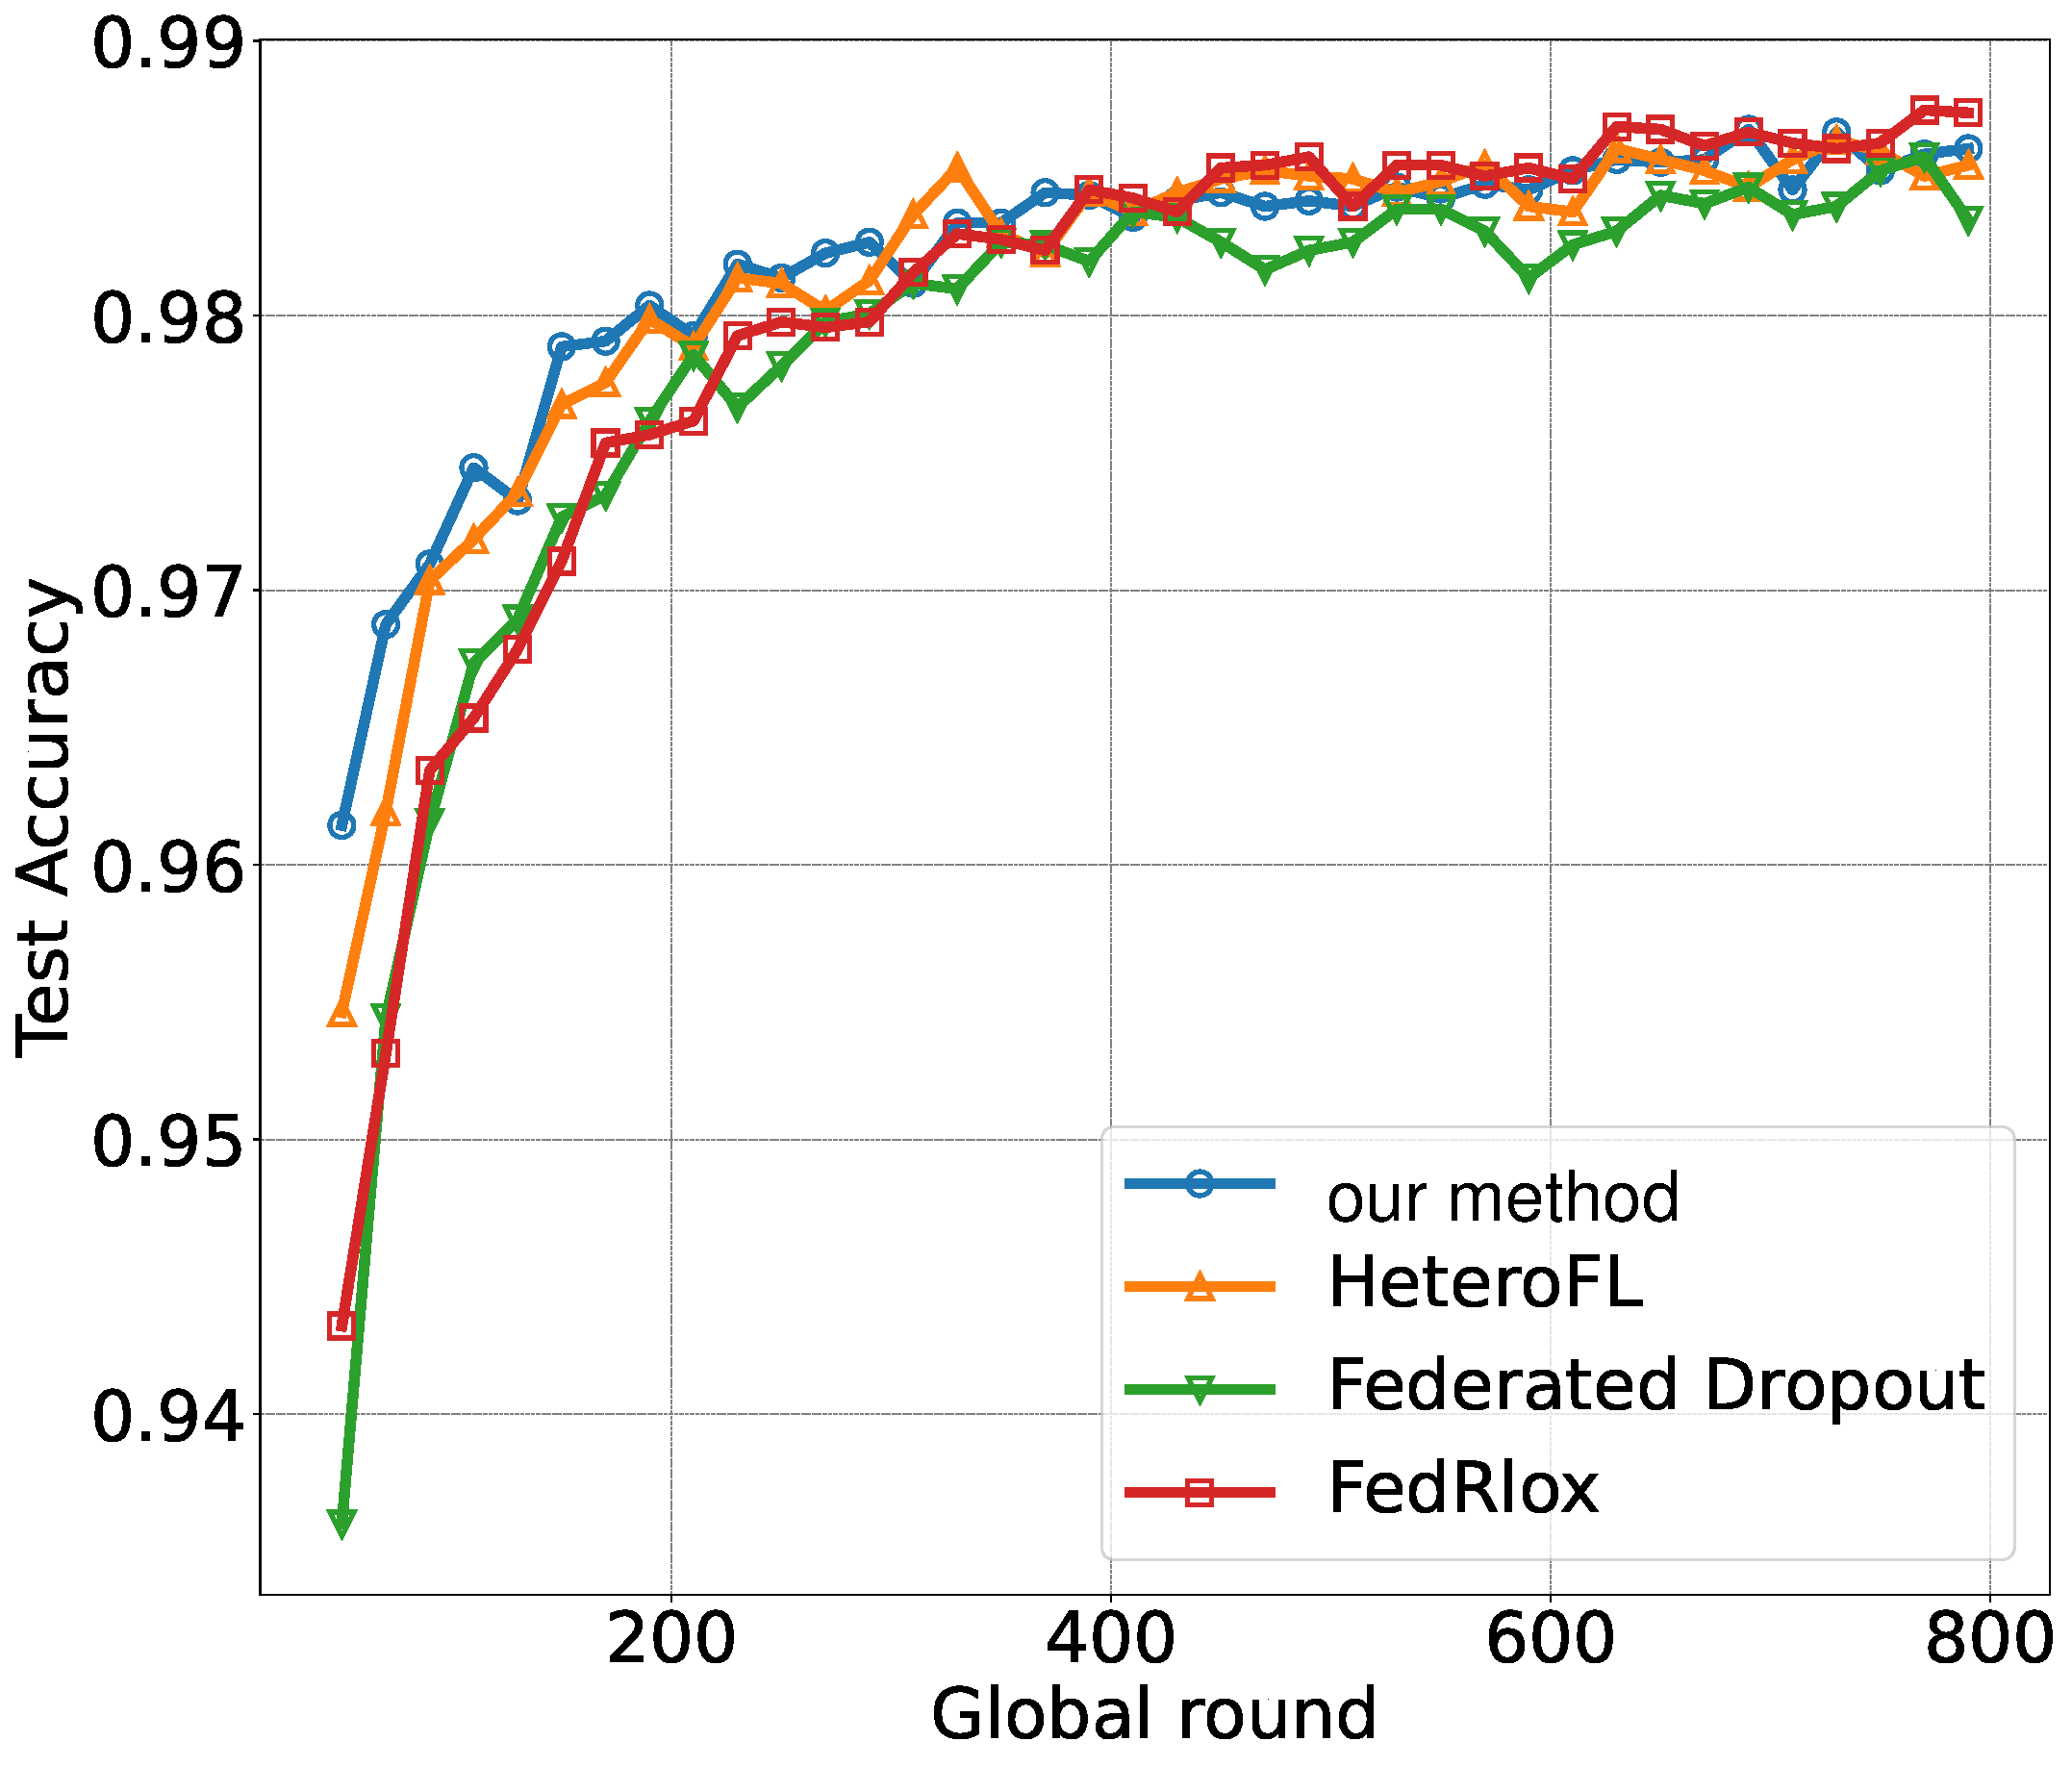
\includegraphics[width=0.9\linewidth]{picture/emnist-low-4.pdf}  
%     }
%     \end{minipage}
%     \hfill  
%     \begin{minipage}{0.45\textwidth}
%     \subfloat[$\rho = 0.6$]{%  
%         \label{fig:emnist-low-0.6}  
%         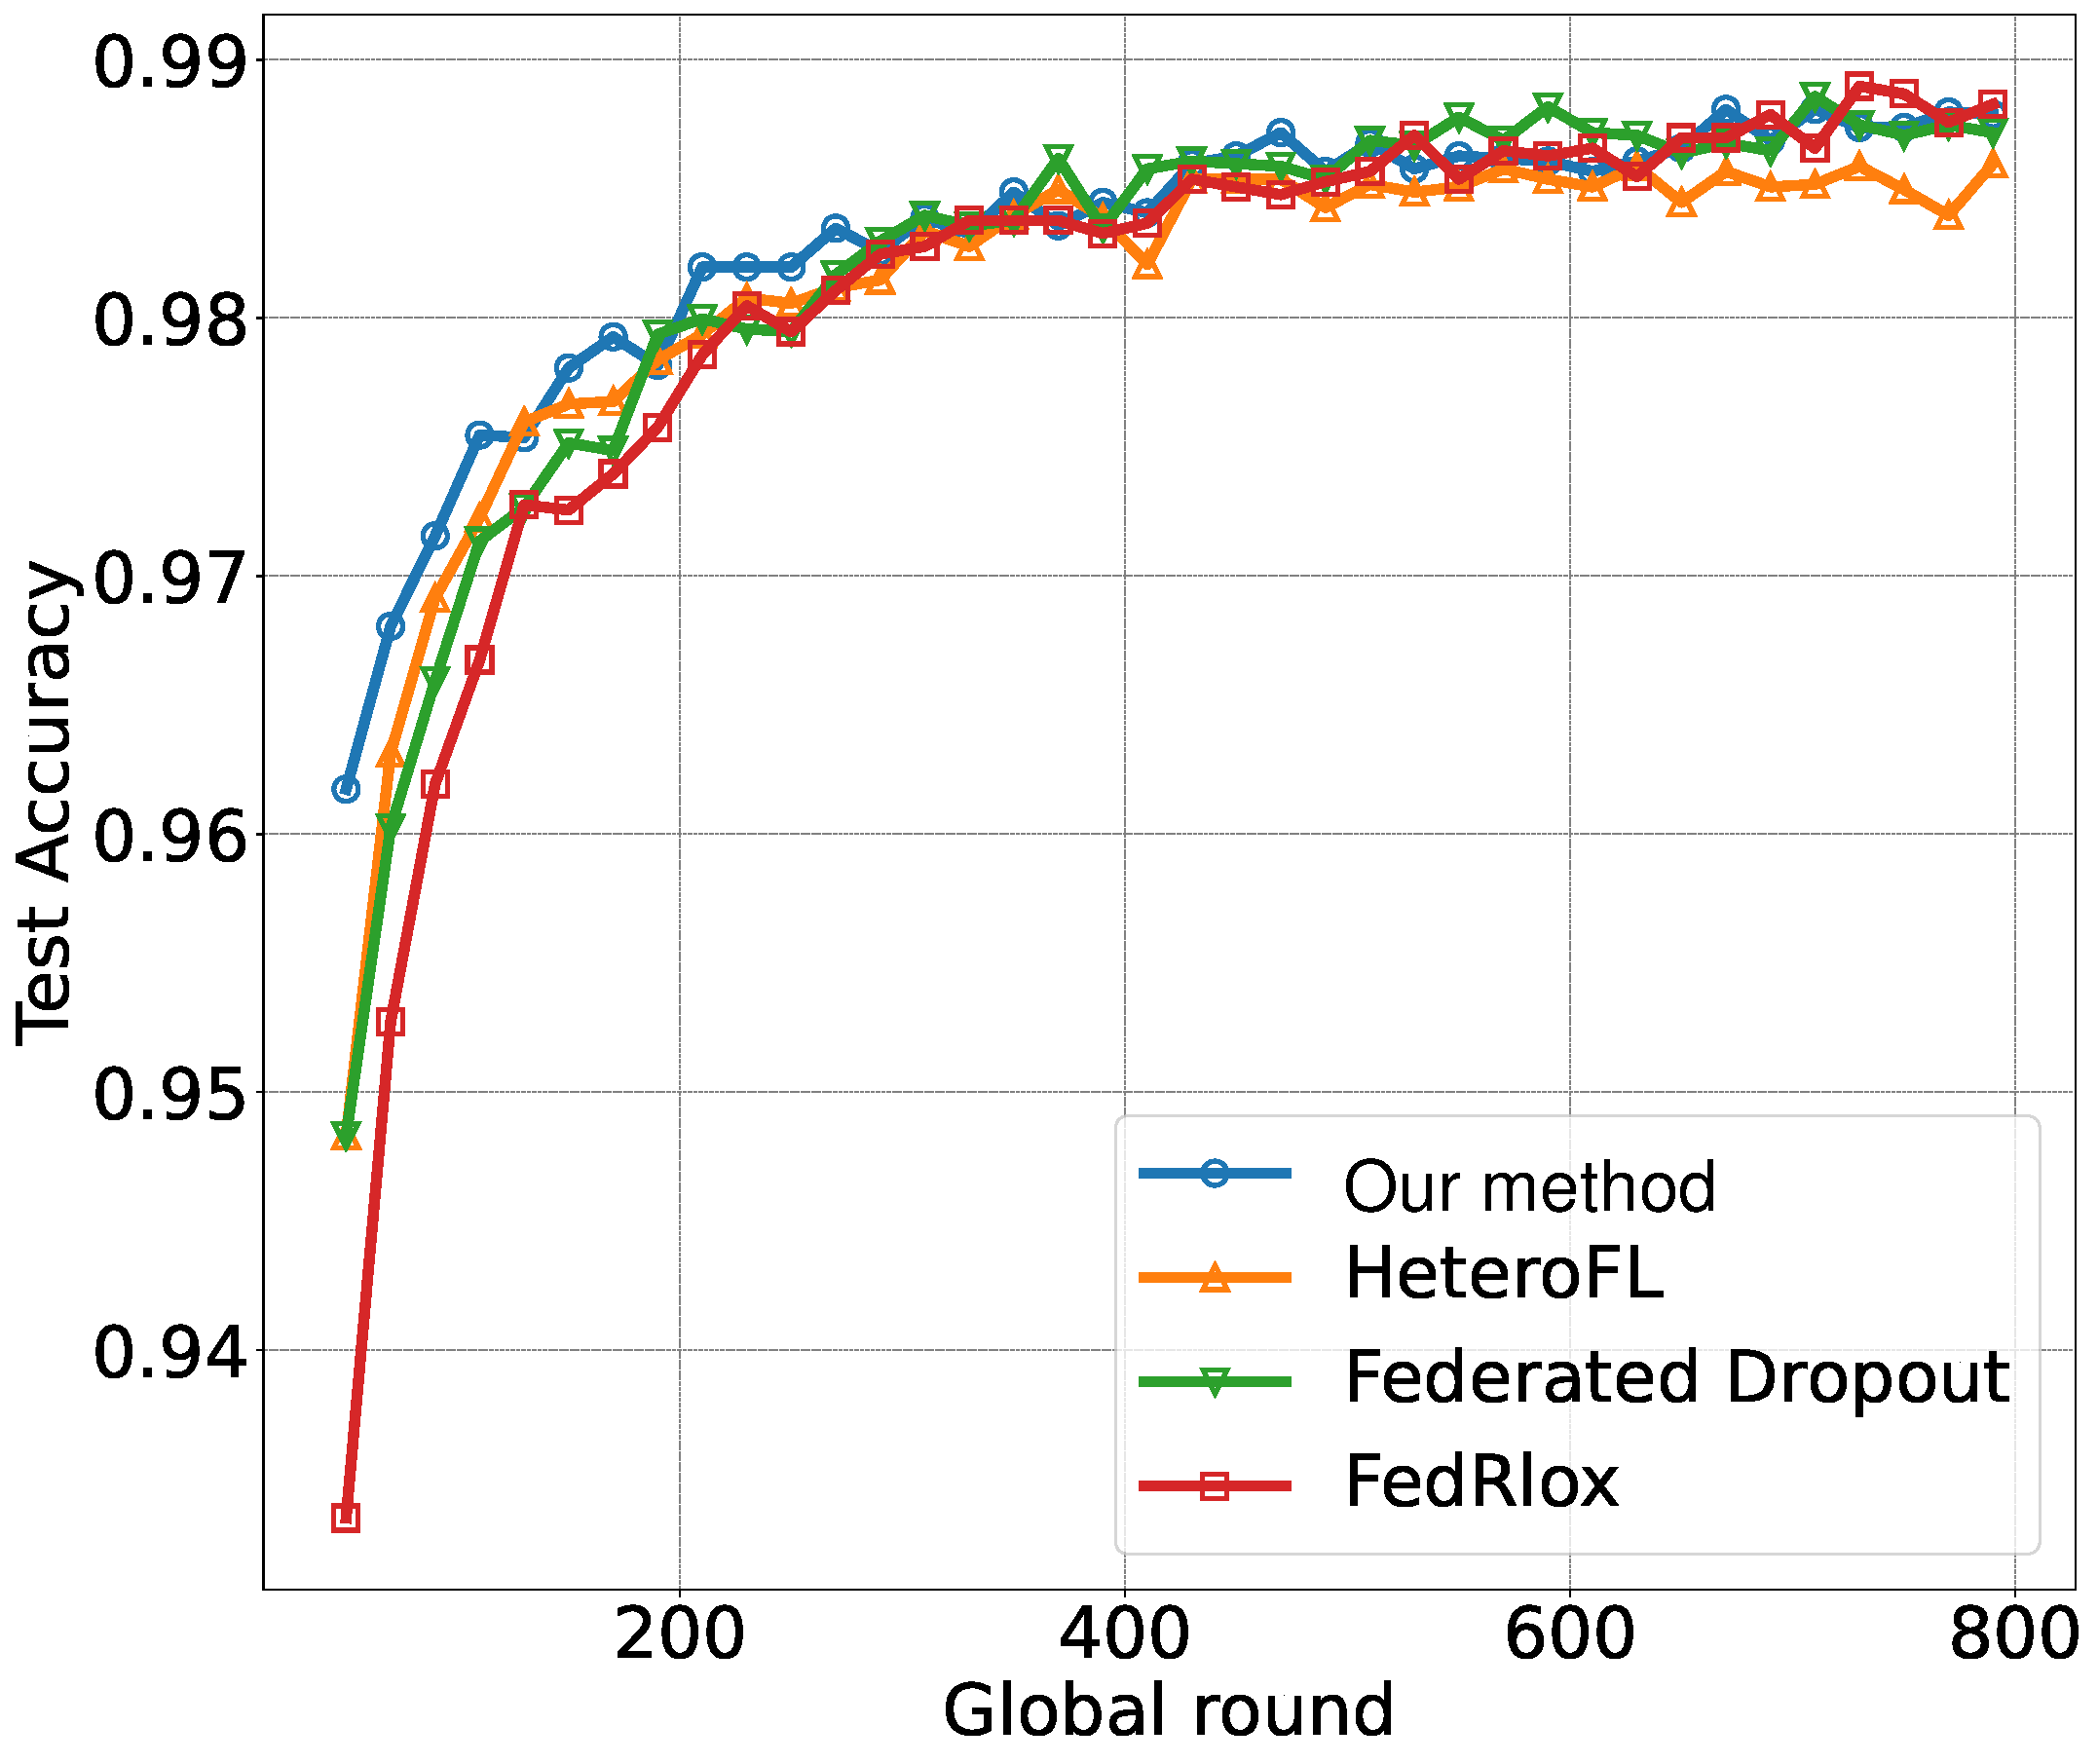
\includegraphics[width=0.9\linewidth]{picture/emnist-low-6.pdf}  
%     }  
%     \end{minipage}
%     \hfill  
%     \begin{minipage}{0.45\textwidth}
%     \subfloat[$\rho = 0.8$]{%  
%         \label{fig:emnist-low-0.8}  
%         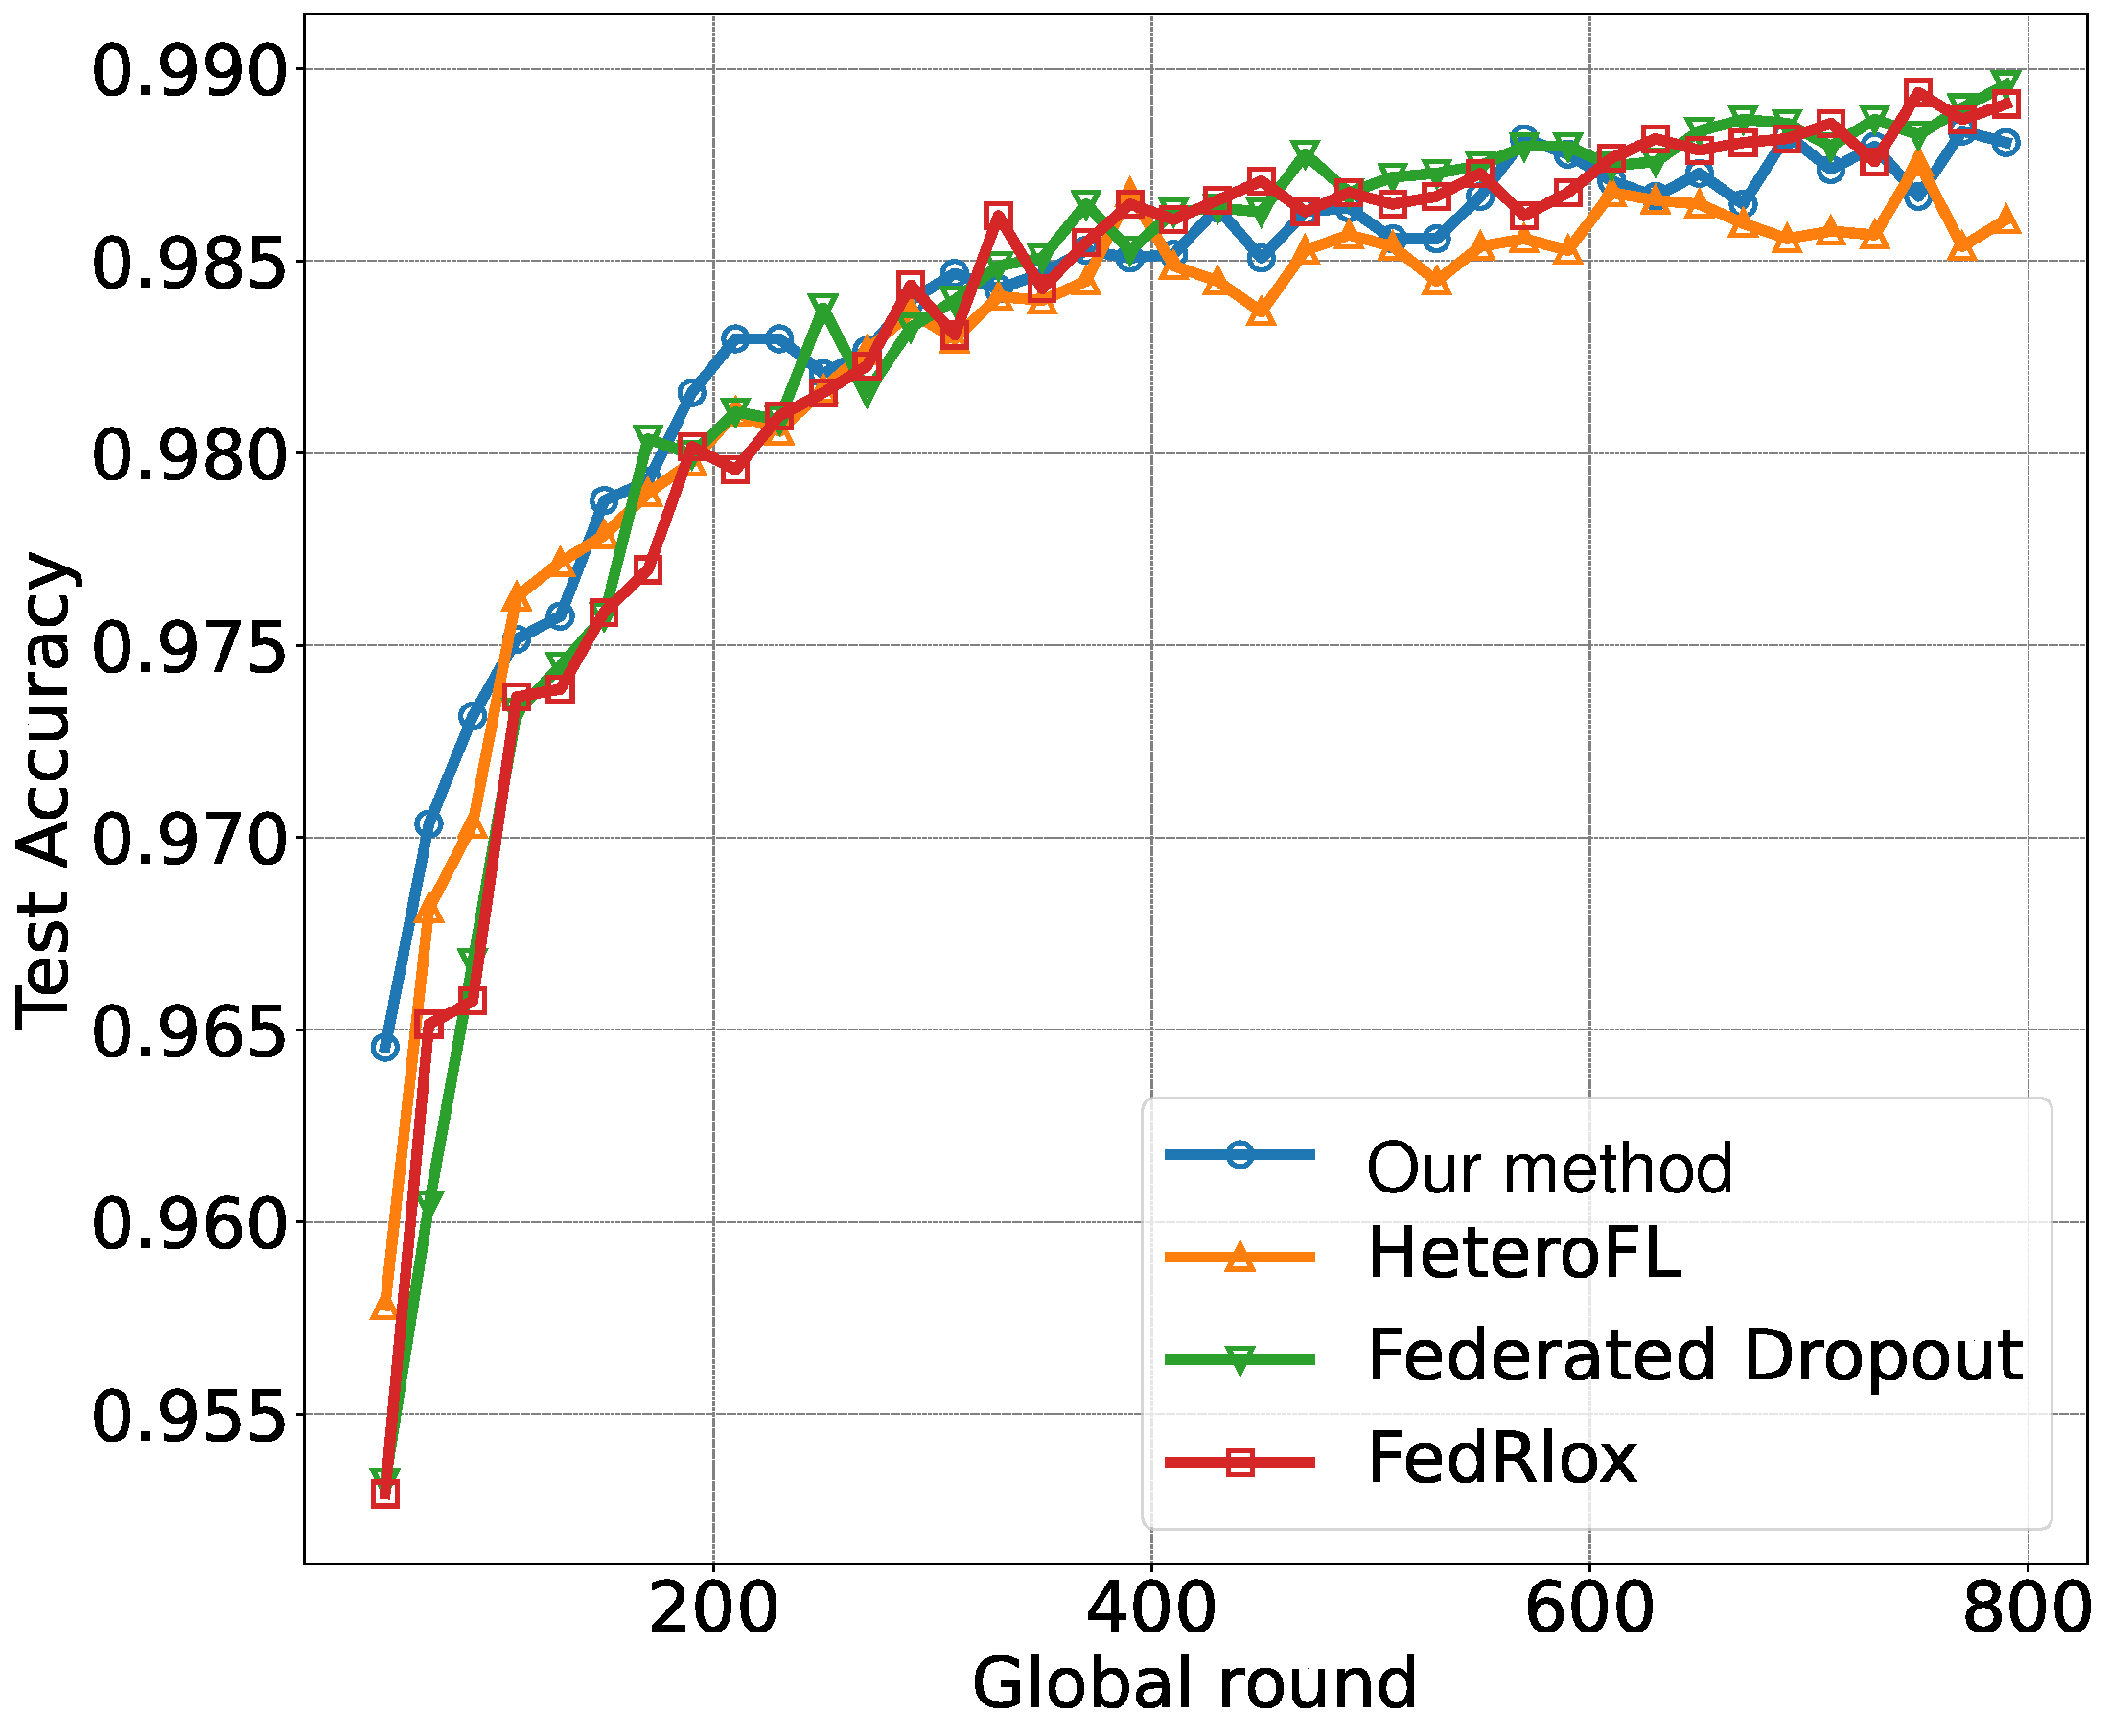
\includegraphics[width=0.9\linewidth]{picture/emnist-low-8.pdf}  
%     }  
%     \end{minipage}
%     \caption{低数据异质性下EMNIST数据训练细节}  
%     \label{fig:emnist-low-low} % 整个图的标签  
% \end{figure}  
%ppppppppppppppppppppppppppppppppppppppppppppppp


\subsection{客户挑选比例对准确率的影响}
为了探究每轮训练过程中选择通信客户端数量的影响,
我们将
frc(表示通信客户端占总客户端的比例)设置为
$\{ 0.05, 0.10, 0.15, 0.20 \} $。
\begin{figure}[thbp]
    \centering
    \subfloat[EMNIST]{%
        \begin{minipage}{0.48\textwidth}
        \centering
        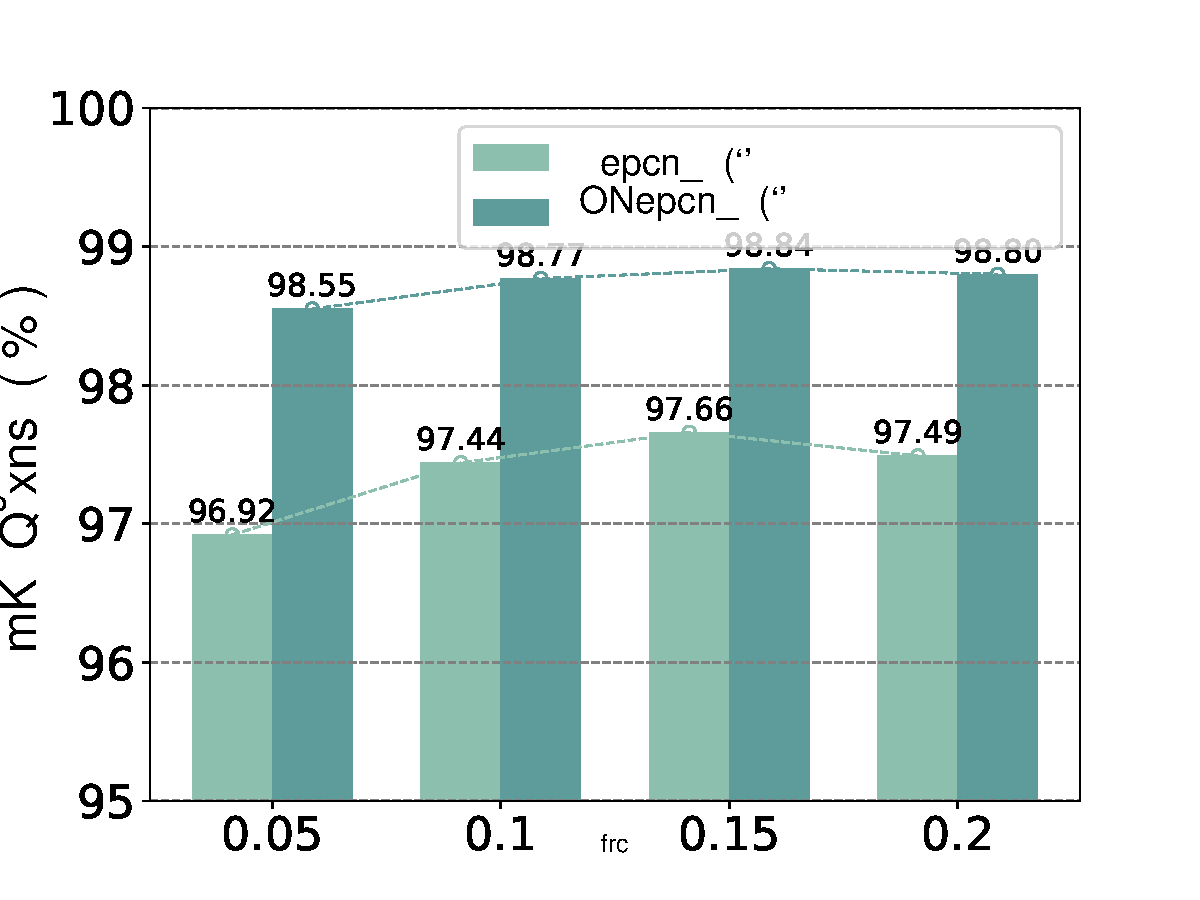
\includegraphics[width=\textwidth]{chapter4/frc_emnist_1616.pdf}
        \label{fig:frc_emnist}
        \end{minipage}
    }
    \hfill
    \subfloat[CIAFR10]{%
        \begin{minipage}{0.48\textwidth}
        \centering
        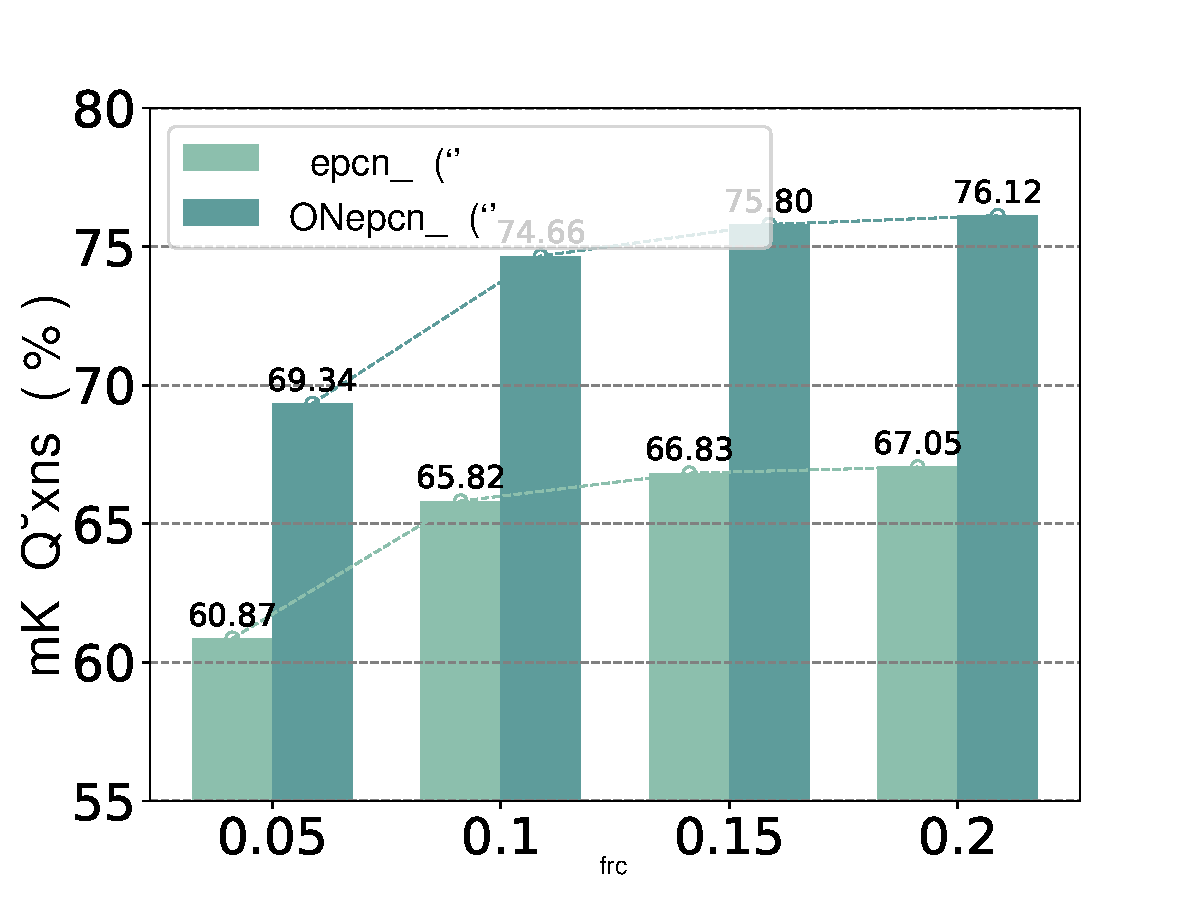
\includegraphics[width=\textwidth]{chapter4/frc_cifar_1616.pdf}
        \label{fig:frc_cifar}
        \end{minipage}
    }
    \hfill
    % \vspace{-0.5cm}
    \caption{客户挑选比例对准确率的影响}
    \label{fig:frc}
    % \vspace{-0.5cm}
\end{figure}
我们将客户端总数设置为100,
每轮对应的通信客户端数量分别为
\{ 5, 10, 15, 20 \}。
图\ref{fig:frc_emnist}和图\ref{fig:frc_cifar}展示了实验结果。
我们可以得出以下三个结论:
(1)当
$frc=0.05$
全局模型准确率明显低于
$frc=\{ 0.10, 0.15, 0.20 \}$
这表明,当通信客户端数量相对较少时,
全局模型中更新的参数较少,从而导致准确率下降。
(2)当frc从
0.10
增加时,
全局模型准确率保持在相对相同的水平,
有时甚至会下降。
这是因为当frc超过0.1时,
有足够的通信客户端参数在全局模型中更新,
因此准确率保持在一个稳定的水平。
当frc继续增加时,参数之间的竞争加剧,有时会导致准确率下降。
(3)
当frc增加到0.2时,
从图\ref{fig:frc_emnist}和图\ref{fig:frc_cifar}中可以观察到,
所有准确率比较都显示出与之前相比的轻微波动或显著下降。
这是因为当每轮中有更多的客户端时,
客户端之间可能会对同一神经元进行更新,从而导致准确率下降。

\subsection{反向传播数据规模对准确率的影响}
\begin{figure}[thbp]
    \label{fig:rho}
    \centering
      \subfloat[EMNIST\label{fig:similardata_emnist}]{  
        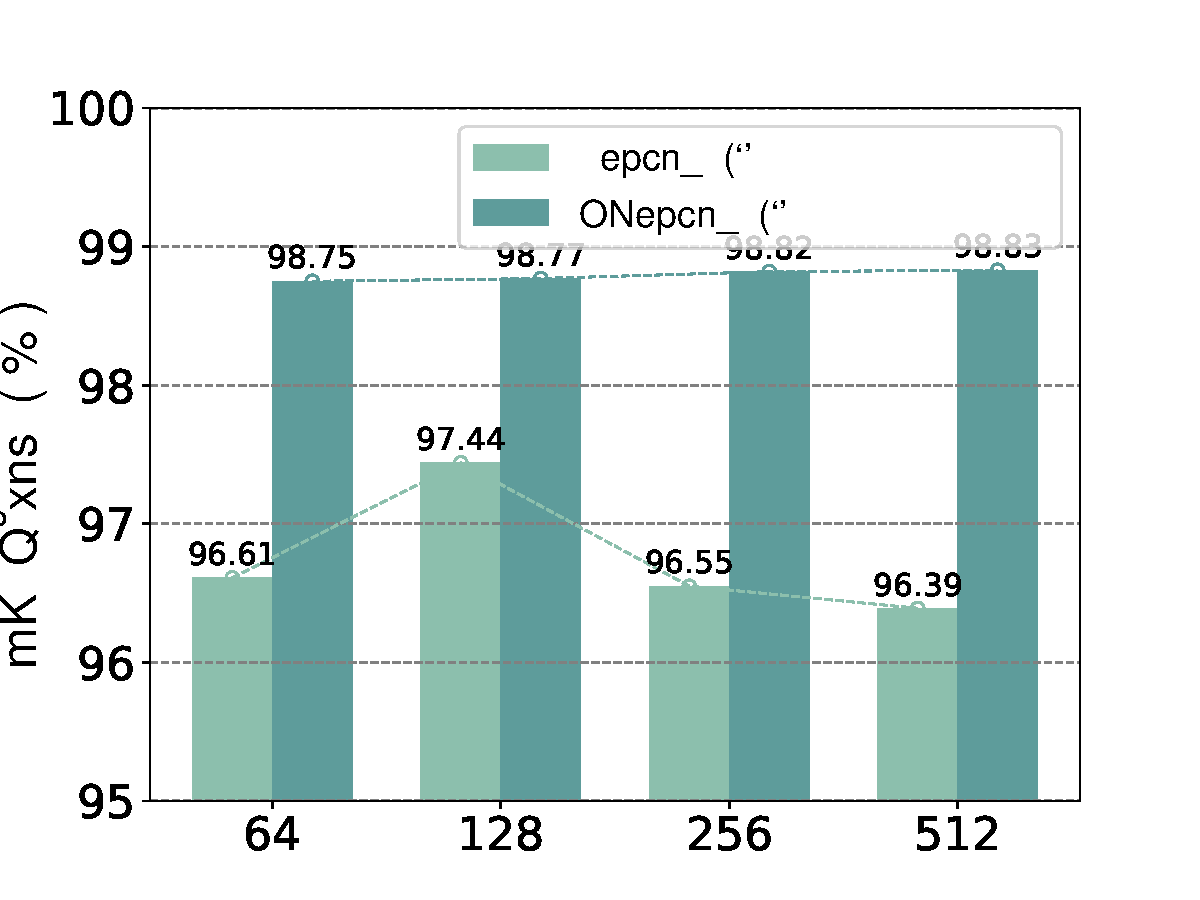
\includegraphics[width=0.45\linewidth]{chapter4/similardata_emnist_1616.pdf}  
      }  
      \hfill
      \subfloat[CIFAR10\label{fig:similardata_cifar}]{  
        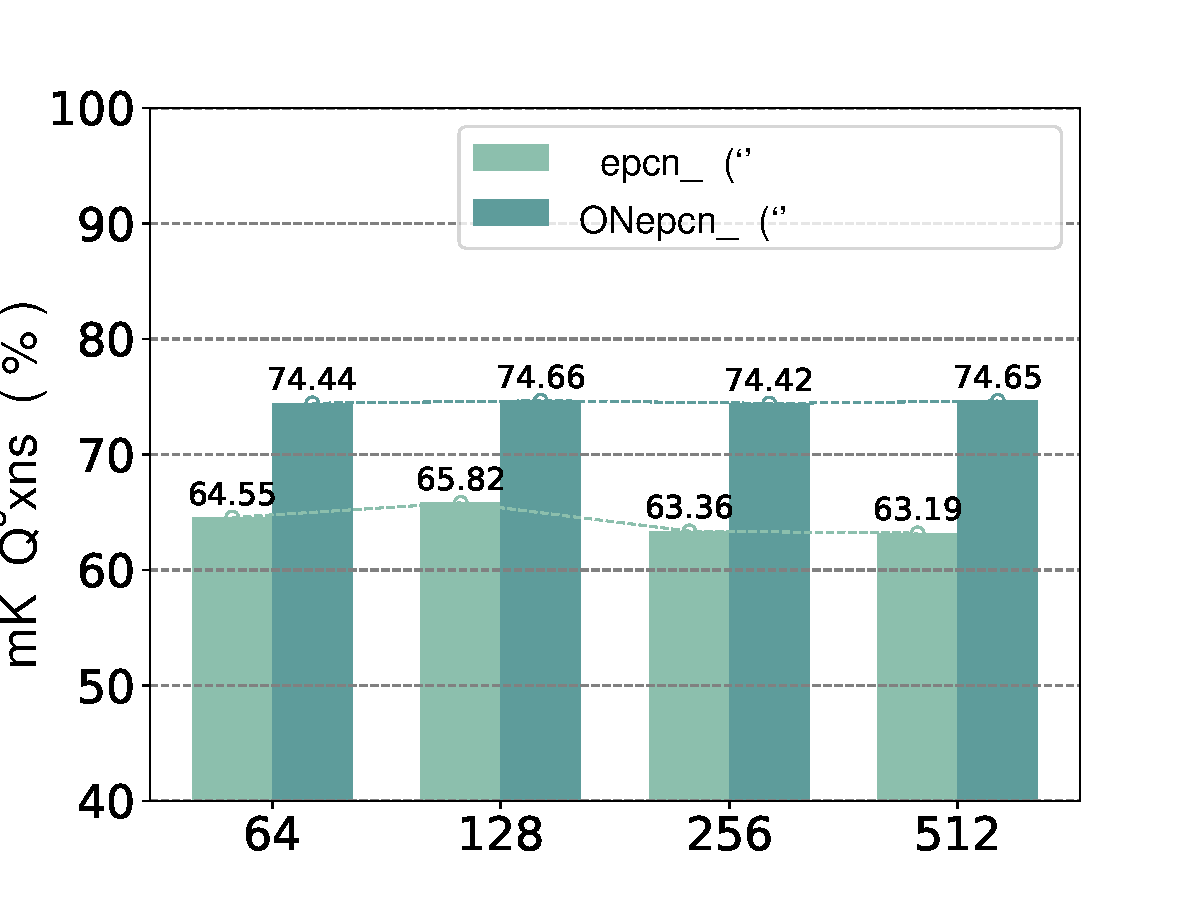
\includegraphics[width=0.45\linewidth]{chapter4/similardata_cifar_1616.pdf}  
      }  
         \caption{  
            推理数据规模对准确率的影响
      }
\end{figure}
我们设置不同数量的相似数据探究这对全局模型准确率的影响。
这些数据是指每次在抽选子模型时候,
我们选择多少规模的数据进行反向传播,
利用这些数据得到的梯度开展子模型抽取工作。
图\ref{fig:similardata_emnist}和图\ref{fig:similardata_cifar}的实验结果显示,
当相似数据的数量从
64变化到512时,
我们可以观察到低数据异质性并未受到显著影响,全局准确率保持在同一水平。
这是因为低数据异质性具有更均衡的分布,
因此改变相似数据的大小对选择重要神经元的能力影响较小,
当数据处于低数据异质性的时候,无论选择多少数据进行方向传播,
只要不是数量过于少,都能得到比较均匀的分布数据,抽取的子模型的波动也会更少。
然而,在高异质性数据上,相似数据的大小导致了全局准确率的显著波动。
高异质性数据的分布更加集中,
相似数据的大小和质量在选择重要神经元方面起着至关重要的作用,
也就是说明如果在少量的数据中没有抽取到当前客户端最相似的数据,
那么抽取的子模型就会与本地数据产生很大的偏离,从而造成训练效果变差。
这意味着选择适当大小的相似数据比拥有更大的数量更为重要,
因为可以最大限度的保证使用最相似数据进行反向传播。
此外,数据的质量以及相似数据与客户端数据集之间的相似性也是影响准确率的重要因素。

\subsection{统计异质性的影响}

\begin{table}[thbp]
    \caption{\label{tab:clientDataDis}FedGSE不同数据集训练参数设置}
    \begin{tabularx}{\linewidth}{l X<{\centering} X<{\centering} X<{\centering} X<{\centering} X<{\centering}}
        \toprule
        \multirow{2}{*}{\textbf{数据集}} & \multicolumn{5}{c}{\textbf{客户数据集包含种类数}} \\ \cline{2-6}
        & 2 & 4 & 6 & 8 & 10\\
        \midrule
        emnist-conv & 97.44 & 98.77 & 98.94 & 98.81 & 99.01 \\
        cifar10-resnet & 65.82 & 74.66 & 75.04 & 76.38 & 74.38 \\
        \bottomrule
    \end{tabularx}
\end{table}
为了研究数据异质性程度对模型准确率的影响,
我们进行了表\ref{tab:clientDataDis}中的实验。
我们将s(客户端本地数据集中包含的类别数量)从2变化到10。
从实验结果中可以看出,当
s从2变化到4时,
全局模型准确率经历了一个显著的跳跃,之后准确率保持在一个稳定的阶段,
表选为略有提升或者有着轻微的下降。
实验结果表明,数据异质性程度对模型的影响存在一个阈值,
当超过这个阈值时,其影响程度会降低。
显然,EMNIST和CIFAR10的阈值都是$s=2$。
可以观察到,在达到阈值后,准确率没有发生显著变化。
这表明FedGSE在处理非独立同分布(non-IID)数据方面具有优势,
即使在数据异质性较低且数据均匀分布的情况下,它也能达到相似的性能水平。
这清楚地展示了我们算法设计的优越性。

\section{本章小结}
在本文中,我们重点研究了全局模型与提取模型之间的更新关系。
然后,我们设计了FedGSE,旨在使子模型的更新尽可能接近全局模型。
我们通过理论证明,使用我们的方法更新的参数最接近全局模型。
大量实验验证了我们的方法在多种方法中表现最优。
然而,仍有一些局限性需要在未来的工作中进一步改进。
具体来说,我们的方法需要在服务器上构建公共数据集。
未来,我们将努力使用生成模型来解决这一问题。